\documentclass[letterpaper,12pt,spanish]{article}

\usepackage[utf8]{inputenc}
\usepackage{graphicx}
\usepackage[spanish, es-tabla]{babel}
\usepackage{amssymb, amsmath, amsbsy} % simbolitos
\usepackage{upgreek} % para poner letras griegas sin cursiva
\usepackage{cancel} % para tachar
\usepackage{mathdots} % para el comando \iddots
\usepackage{mathrsfs} % para formato de letra
\usepackage{stackrel} % para el comando \stackbin
\usepackage{float}
\usepackage{listings}
\usepackage{color}
\usepackage{vmargin}
\usepackage[bookmarks = true, colorlinks=true, linkcolor = black, citecolor = black, menucolor = black, urlcolor = black]{hyperref} 
\usepackage{multirow} % para las tablas
\usepackage{pdflscape}
\usepackage[final]{pdfpages}
\usepackage{booktabs}
\usepackage{enumitem}
\usepackage[table,xcdraw]{xcolor}
\usepackage{multicol} 



\usepackage{pgfgantt}
\usepackage{tikz}
\usetikzlibrary{calc}

\usepackage{amsfonts}

\usepackage{geometry}
\usepackage{graphicx}

\setpapersize{USletter}
\setmargins{2.5cm}       % margen izquierdo
{1.5cm}                        % margen superior
{16.5cm}                      % anchura del texto
{23.42cm}                    % altura del texto
{10pt}                           % altura de los encabezados
{1cm}                           % espacio entre el texto y los encabezados
{0pt}                             % altura del pie de página
{0.5cm}                           % espacio entre el texto y el pie de página

\providecommand{\keywords}[1]{\textbf{\textit{Palabras clave---}} #1}

\title{Aplicación móvil para la comunicación con personas que utilizan el lenguaje de señas.}
\author{Lemus Pichardo Oscar Alejandro}

\begin{document}

\pagenumbering{gobble}
%
\includepdf[pages=1,pagecommand={},offset=2.5cm -3cm]{coverpage/Thesis}
%
\includepdf[pages=2,pagecommand={},offset=2.5cm -3cm]{coverpage/Thesis}
%
\includepdf[pages=3,pagecommand={},offset=2.5cm -3cm]{coverpage/Thesis}



\begin{abstract}

En este trabajo se presenta el diseño de una aplicación móvil que permitirá la comunicación básica entre personas que usan el lenguaje de señas mexicano con personas que no lo utilizan mediante el reconocimiento de voz y una entrada por texto para su posterior síntesis de voz.

El reconocimiento de voz se lleva a cabo en un servidor que se comunica con la aplicación a través de un servicio web, el reconocimiento se lleva a cabo con una red neuronal \textit{feedforward Pattern Recognition} teniendo como entrada los coeficientes cepstrales en la frecuencia de MEL cuantizados vectorialmente. La adquisición de la señal de voz se realiza con una frecuencia de muestreo de 8 kHz con 8 bits de PCM. Las palabras reconocidas se presentarán en la pantalla del móvil en forma de imágenes que corresponden a las señas del diccionario de lengua de señas mexicana de la CONAPRED.

La aplicación móvil realiza la síntesis de voz de mensajes escritos haciendo uso de la API de Google y además presenta un diccionario auxiliar que informa sobre el cómo realizar la seña de diferentes palabras por categorías.

\keywords{Lengua de señas, Red neuronal, Reconocimiento de voz, Aplicación móvil}
\end{abstract}

\tableofcontents % indice de contenidos

\newpage
%\cleardoublepage
%\addcontentsline{toc}{chapter}{Lista de figuras} % para que aparezca en el indice de contenidos
\listoffigures % indice de figuras

%\cleardoublepage
%\addcontentsline{toc}{chapter}{Lista de tablas} % para que aparezca en el indice de contenidos
\listoftables % indice de tablas
\renewcommand{\thesection}{\Roman{section}} 

\pagenumbering{arabic}
\setcounter{page}{10}
\section{Introducción}

	Una de las necesidades principales del ser humano es la de la comunicación, éste tiene la necesidad de ser escuchado y de interactuar con los demás seres vivos en especial con otros humanos, la comunicación nos ayuda a compartir sentimientos, es una forma de expresarnos \cite{VelezMelendez2004}.

	En la vida diaria tenemos diversas formas de comunicarnos, puede ser con señales acústicas (voz, sonidos, ruidos), visualmente, por medio de medios impresos, la escritura, dibujos, señas, etc. El objetivo es mandar un mensaje, básicamente se puede describir la comunicación mediante el diagrama de la Figura \ref{comunicacion}.

	\begin{figure}[H]
		\centering
		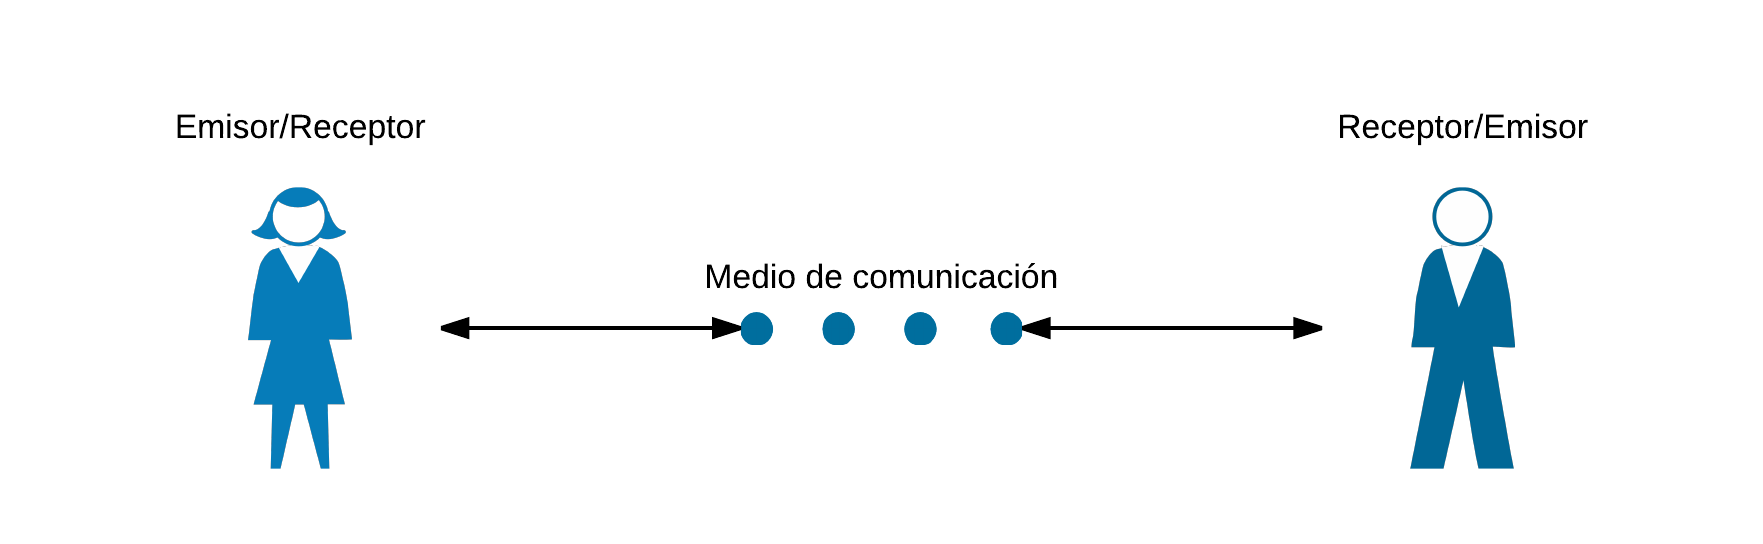
\includegraphics[scale = 1]{figures/Comunicacion}
		\caption{Elementos de comunicación.}
		\label{comunicacion}
	\end{figure}

	La comunicación oral nos ofrece grandes ventajas sobre los demás métodos de comunicación pues es el modo de comunicación más natural entre nosotros los humanos, la gran ventaja es que no es necesario estudiarla, es parte de nuestro crecimiento, aprendemos a hablar, adoptamos el idioma, el acento, las costumbres, en cambio el modo de comunicación escrita requiere de un estudio del alfabeto, escritura y lectura, además de que la comunicación oral nos permite inducir más significados a las palabras que su propia definición gracias al tono de voz \cite{CamargoLopez}.

	Pero no todos tenemos la capacidad de comunicarnos de forma oral, hay personas que no pueden hablar u oír ya sea porque nacieron con esta deficiencia o porque por alguna razón físicamente se vieron limitados a realizar tal actividad.

	La discapacidad es una condición que puede afectar a cualquier miembro de la sociedad sin importar edad, sexo, estatus social-educativo-laboral o educación geográfica \cite{Flores}. Como consecuencia se tienen deficiencias en el rendimiento de la actividad cotidiana de la persona como en la ejecución de tareas, actitudes y conductas \cite{Flores}.

	Desarrollar una aplicación móvil que pueda eliminar esta barrera de comunicación puede ser una herramienta muy útil para que las personas con discapacidad auditiva no pierdan la comunicación o aprendan a comunicarse con el resto de las personas y de esta forma la interacción no esté limitada en ambos sentidos.

\section{Planteamiento del problema}

La Organización Mundial de la Salud (OMS) estima que hay más de 300 millones de personas con discapacidad auditiva en el mundo. Y de acuerdo al XIII Censo General de Población y Vivienda 2010, existen un total de 498 mil 640 personas sordas en México, donde 273 mil 216 son hombres y 225 mil 424 son mujeres \cite{Valencia2012}. La mayoría de estas personas vive en condiciones precarias, lo cual acentúa la falta de acceso a la educación superior. La Dirección de Educación Especial de la Secretaría de Educación Pública (SEP) está a cargo de instruir a las personas sordas, sin embargo, sólo se oferta hasta el nivel básico de secundaria por lo que al egresar estas personas no tiene opción para continuar \cite{Miranda2003}.

	Otro problema presente en esta población es que no existe  vocabulario científico ni técnico para explicar ciertos procesos a nivel preparatoria, además también se enfrentan al problema que se relaciona con las nociones de lengua escrita que reciben en el aula, pues no les son suficientes para leer y escribir de forma adecuada, lo cual obstaculiza su ingreso al nivel medio superior \cite{Miranda2003}.	

	Debido a la falta de interés de las personas en aprender el lenguaje de señas las personas que sufren esta deficiencia del habla quedan excluidas de la sociedad en general, pues sólo pueden establecer comunicación con grupos especiales que dominan este sistema de señas.

	Estas personas quedan excluidas debido a que no logran una adaptación completa en la sociedad pues no pueden comunicarse con los demás, expresarse o hacer que los demás los escuchen, y una solución podría ser que todos aprendamos este lenguaje, el problema es la falta de educación orientada a este aspecto y el desinterés en esta lengua. 


	Por otro lado, las personas que pierden la audición pueden tener algunos problemas sociales como:

	\begin{itemize}
		\item Aislamiento y retraimiento.
		\item Pérdida de atención.
		\item Falta de concentración.
		\item Problemas en el trabajo.
		\item Problemas de comunicación.
	\end{itemize}


	Por lo que se plantea la pregunta ¿Cómo realizar una aplicación que utilice el reconocimiento de voz para facilitar la comunicación entre personas que no utilizan el lenguaje de señas con personas que sí?

\section{Propuesta de solución}

	La solución propuesta consiste en una aplicación móvil en la plataforma Android, la cual nos ayudará a realizar la interpretación de voz a lenguaje de señas y la síntesis de voz a partir de un teclado.

	Se plantea la situación en la que una persona sorda, muda o sordomuda y una persona que puede escuchar y hablar perfectamente pero no conoce el lenguaje de señas están de frente y desean entablar una comunicación.

	La propuesta es tener una aplicación en el dispositivo móvil que ayude a estas dos personas a llevar a cabo una comunicación básica, con frases comunes. La aplicación contará con un módulo de reconocimiento de voz y bajo entrenamiento podrá reconocer ciertas frases de la comunicación como pueden ser frases para saludar, comprar o pedir indicaciones de la ciudad, y mediante la pantalla del móvil mostrar la imagen correspondiente en lenguaje de señas, de esta forma la persona 1 (persona que utiliza el lenguaje de señas) podrá entender lo que la persona 2 (persona que no utiliza el lenguaje de señas) quiere comunicar (Figura \ref{comunicacionVoz}).

	\begin{figure}[H]
		\centering
		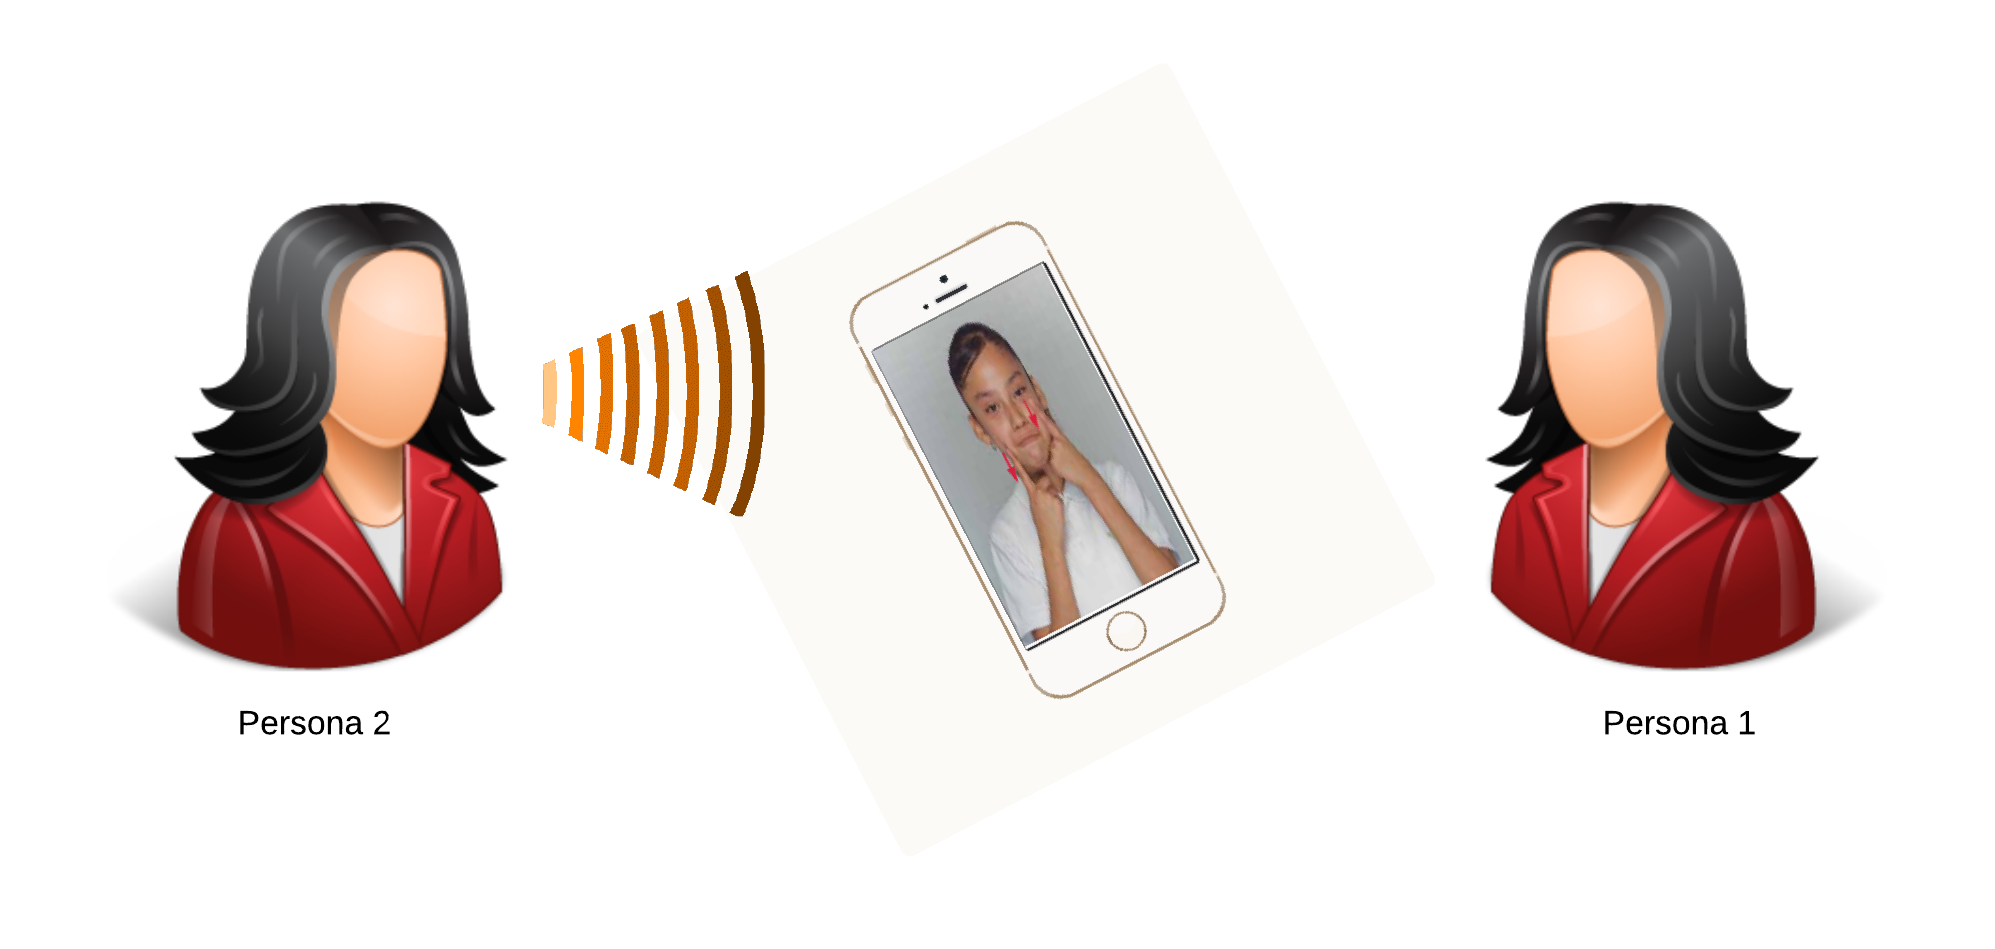
\includegraphics[scale = 0.7]{figures/ComunicacionBA}
		\caption{Comunicación por voz.}
		\label{comunicacionVoz}
	\end{figure}

	Por otra parte, cuando la persona 1 quiera comunicarse con la persona 2, la aplicación en esta sección mostrará un teclado por el cual la persona 1 escribirá la frase que desea comunicar y se sintetizará en voz lo escrito, el módulo se plantea de tal forma que se pueda obtener la comunicación bidireccional y ésta no quede trunca (Figura \ref{comunicacionTeclado}), la implementación de esta sección se hará con el uso de la API de síntesis de voz de Google, de tal manera que el trabajo esté enfocado principalmente en la primera sección que es el reconocimiento de voz. Esto se propone para que la app final permita una comunicación bidireccional.

	\begin{figure}[H]
		\centering
		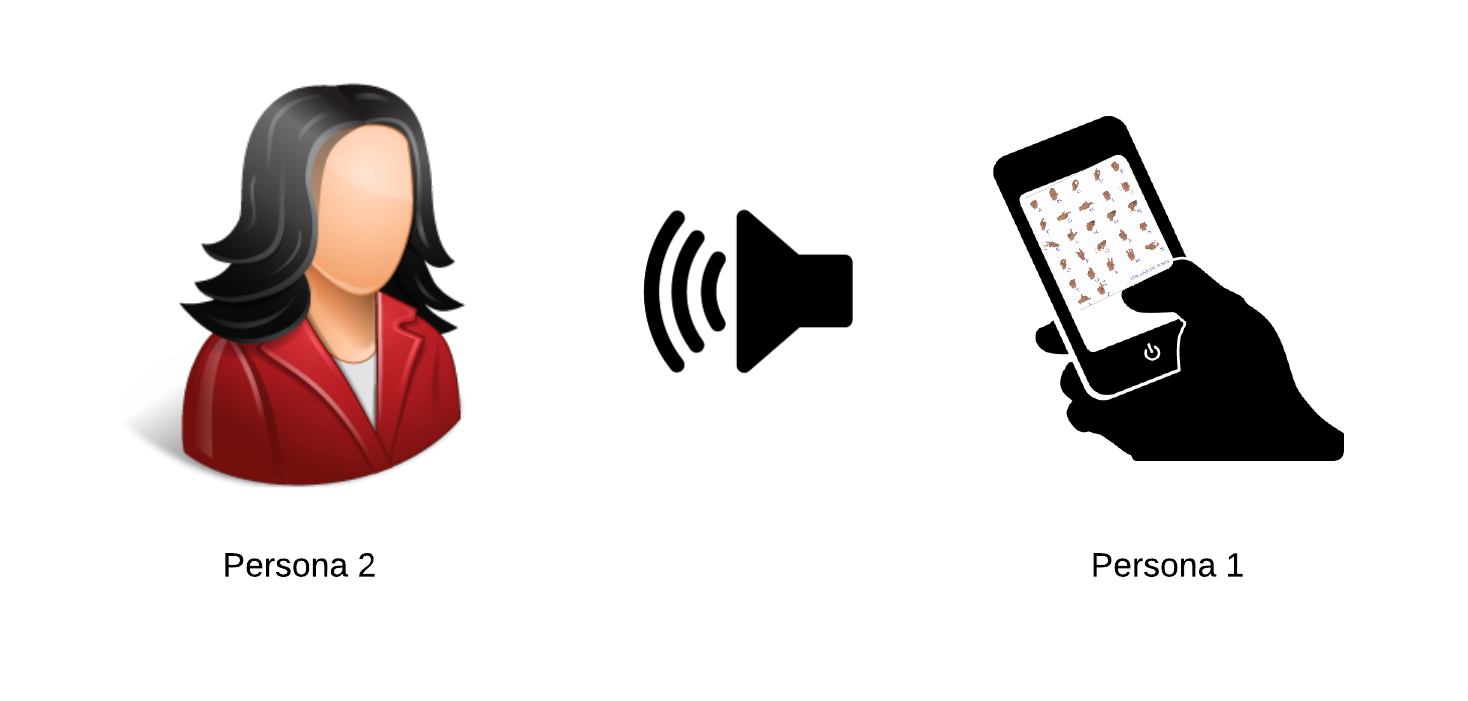
\includegraphics[scale = 0.8]{figures/ComunicacionAB}
		\caption{Comunicación por teclado}
		\label{comunicacionTeclado}
	\end{figure}
	
	Además de los módulos propuestos se plantea que la aplicación cuente con un diccionario, con el cual podremos aprender el lenguaje de señas, palabras, gestos y el cómo utilizarlos.

		\subsection*{Arquitectura del sistema.}
		
		Se puede definir a la aplicación en diferentes módulos, los cuales se pueden observar en las Figuras \ref{vozSenB} y \ref{tecVozB}.
		En la Figura \ref{vozSenB} se explicará cómo sería la arquitectura de la parte de la aplicación donde se va a tener la comunicación por voz.

		\begin{figure}[H]
			\centering
			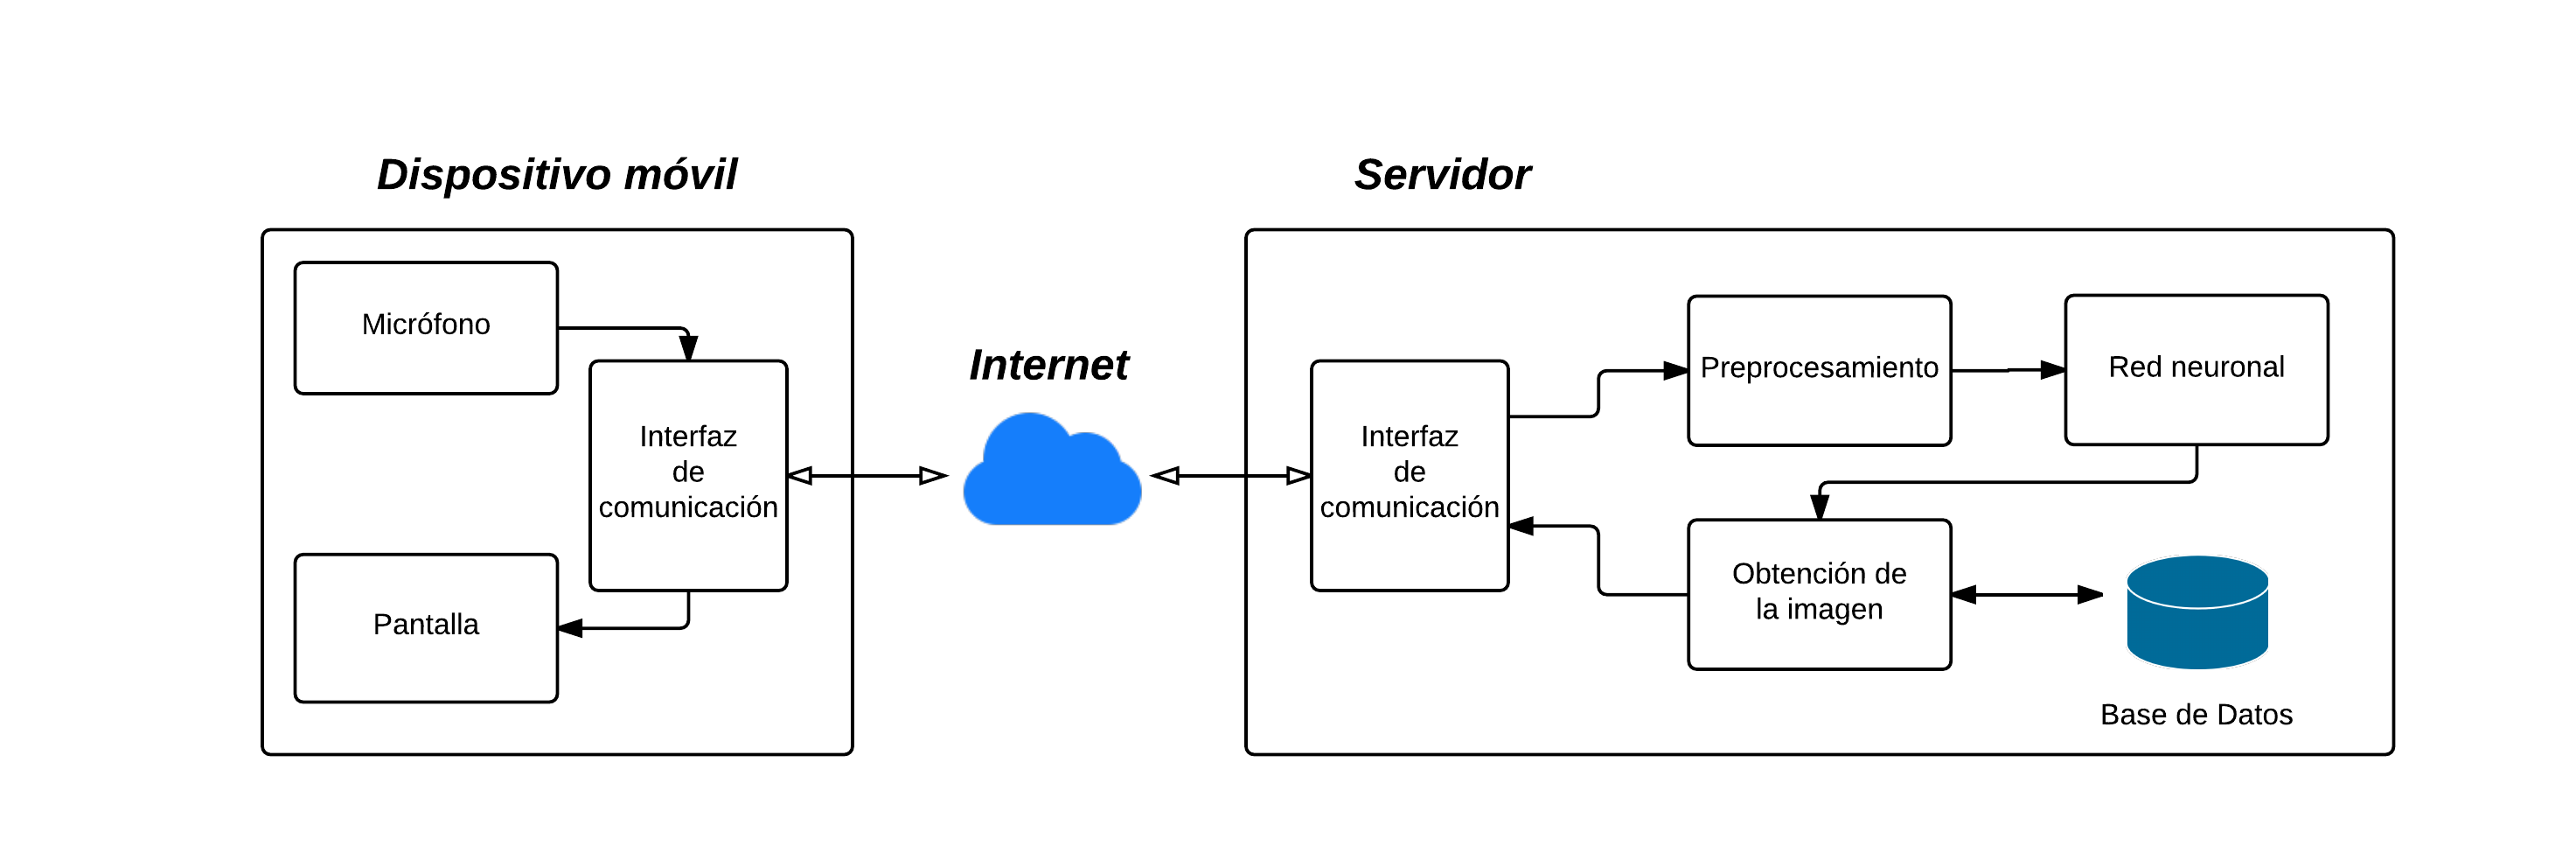
\includegraphics[scale = 0.7]{figures/Etapavoz}
			\caption{Diagrama a bloques del sistema que relaciona voz a imágenes de lenguaje de señas.}
			\label{vozSenB}
		\end{figure}		

		A través del micrófono del dispositivo móvil se va a capturar la señal de voz, esta señal será enviada a través de internet a un servidor que realizará el pre procesamiento de ésta para su posterior reconocimiento y obtención de la imagen correspondiente a la frase identificada, finalmente la imagen recuperada será enviada al móvil para su presentación en la pantalla.
		\paragraph{}

		En la Figura \ref{tecVozB} se presenta la arquitectura del módulo de síntesis de voz donde la entrada del texto es por medio del teclado.

		\begin{figure}[H]
			\centering
			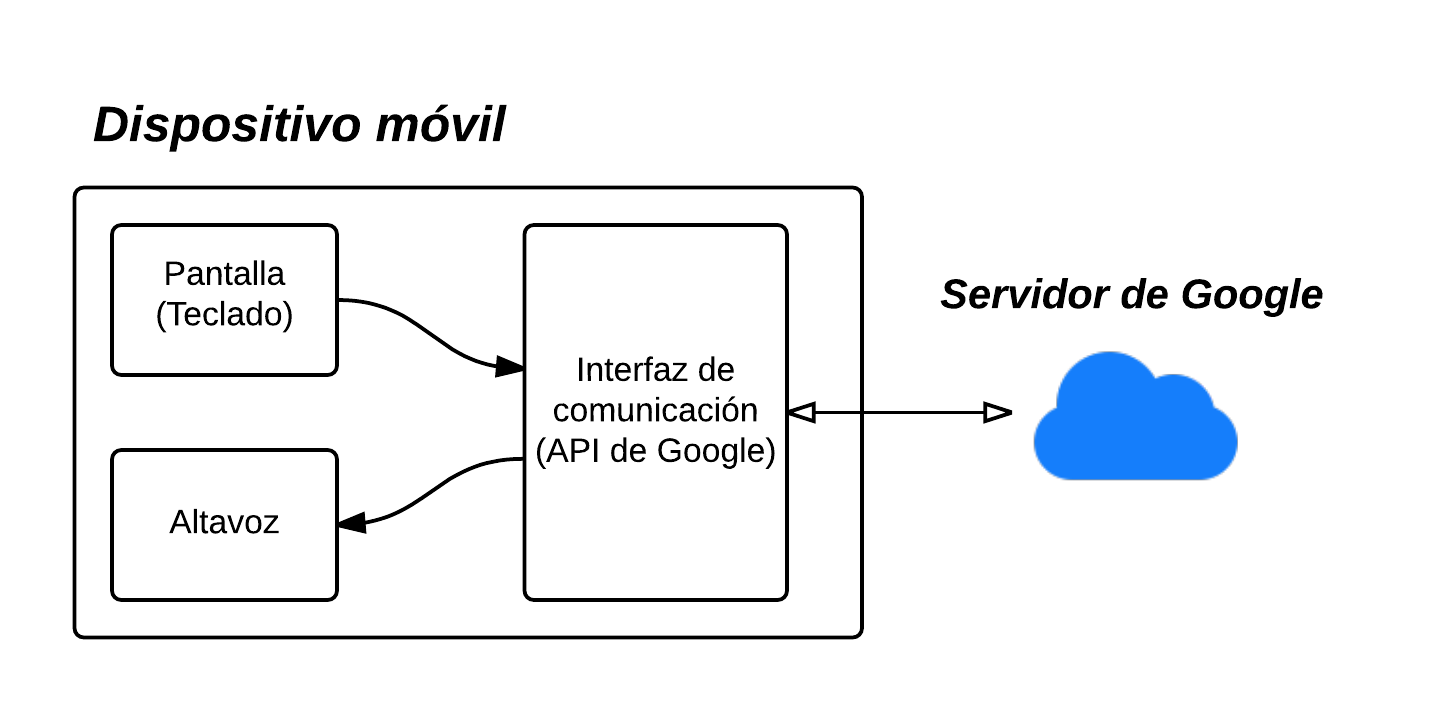
\includegraphics[scale = 0.8]{figures/Etapateclado}
			\caption{Diagrama a bloques del módulo de síntesis de voz con entrada por medio de un teclado.}
			\label{tecVozB}
		\end{figure}	

		Por medio de un teclado presentado en pantalla se tendrá la entrada del texto que se desea comunicar y con ayuda de la API de síntesis de voz de Google  se implementará la síntesis para que la persona 2 escuche lo que la persona 1 quiere comunicar.





	\subsection*{Metodología}
	
	Para implementar la aplicación propuesta se plantea realizar las siguientes actividades.

	\begin{itemize}
		\item Reconocimiento de voz: Como parte del pre procesamiento se hará un análisis de las características de la voz que debemos tratar para realizar dicho reconocimiento, de este análisis implementaremos determinados filtros que nos ayuden a preparar la señal de voz para el adecuado procesamiento. Se estudiarán las redes neuronales adecuadas para llevar a cabo el reconocimiento de frases. El entrenamiento y validación de la red primeramente se llevará a cabo en Matlab debido a su fácil manejo y después se implementará en el lenguaje de programación C debido a que el desempeño será mejor que la implementación en Java.

		Se opta por el uso de redes neuronales para el reconocimiento de voz debido a que se tiene más experiencia en el tema y de esta forma permitir realizar la aplicación completa dados los tiempos para el desarrollo del proyecto.

		\item Base de datos: Se implementará una base de datos relacional en MySQL que almacenará todo el vocabulario seleccionado del lenguaje de señas relacionado a su texto correspondiente, de esta forma cuando se tenga la frase se pueda solicitar la imagen.

		Se decidió usar MySQL por ser el manejador de bases de datos más versátil de los tres más comerciales\footnote{MySQL, SQL Server y PostgreSQL}, esta decisión se toma con base a los datos mostrados en la tabla \ref{tabla:dbms}.

		\item Síntesis de voz: Se llevará a cabo la implementación de la síntesis de voz de las  frases ingresadas a través del teclado con ayuda de la API de Google, se estudiará el funcionamiento de la API y se analizará la mejor implementación posible que pueda usarse, ya sea mediante una conexión a internet o de forma local.

		\item Aplicación móvil: Se realizará el diseño de la aplicación de tal forma que sea intuitiva, se definirá el modelo de desarrollo que mejor se adapte a la aplicación y se especificarán los requerimientos del sistema.

		\item Conectividad: Se implementará la comunicación entre el servidor y el dispositivo móvil por medio del protocolo TCP-IP para tener acceso a la red y de esta forma poder manipular la base de datos a nuestra conveniencia, de esta forma, la aplicación necesitará la conexión a internet para llevar a cabo el procesamiento, la conexión puede ser tanto por Wi-Fi como por redes móviles.

		\item Integración y validación: Ya teniendo todos los elementos del sistema se llevará a cabo la integración y validación del sistema, básicamente enlazar los puntos principales en el servidor y realizar la conexión con el dispositivo móvil a través de la internet.

		\item Pruebas: Finalmente se llevarán a cabo diversas pruebas en diferentes escenarios en los que se requiera la comunicación entre personas que presentan la deficiencia para hablar y las personas que no la presentan.

		\item Para cuestiones técnicas se hará un análisis de la velocidad de respuesta del sistema de forma teórica, esto tomando la complejidad computacional y la velocidad de procesamiento donde se llevará a cabo el reconocimiento.
	\end{itemize}

\section{Objetivos}

		\subsection*{Objetivo general}
			Implementar una aplicación móvil en el sistema operativo Android que permita la comunicación de voz a lenguaje de señas y la síntesis de voz a través de la entrada por teclado mediante la implementación de una red neuronal de reconocimiento de frases, uso de una API de síntesis de voz y el desarrollo de un diccionario básico para facilitar la comunicación entre personas con discapacidad auditiva y personas que no presentan dicha discapacidad.
		\subsection*{Objetivos específicos}
		\begin{itemize}
			\item Definir los requerimientos del sistema.
			\item Analizar la red neuronal óptima para el reconocimiento de voz.
			\item Analizar la API de síntesis de voz para la comunicación a través del teclado.
			\item Diseñar la interfaz gráfica para la aplicación.
			\item Entrenar la red neuronal de reconocimiento de voz e implementarla en lenguaje C para su posterior integración al sistema.
			\item Implementar el teclado y la síntesis de voz para su posterior integración al sistema.
			\item Diseñar la base de datos para establecer la relación entre frases e imágenes.
			\item Establecer la integración del sistema y la comunicación entre el dispositivo móvil y el servidor.
			\item Definir un diccionario básico del lenguaje de señas para agregarlo al sistema.
			\item Realizar pruebas y obtener desempeño del sistema.
		\end{itemize}

\renewcommand{\thesection}{\arabic{section}} 
%\setcounter{section}{0}

	\section{Estado del arte}\label{sec:stateoftheart}
	
	En esta sección se presentan diversas aplicaciones que tienen como objetivo el facilitar la comunicación entre personas que ocupan el lenguaje de señas con las que no, además, se muestran las técnicas y herramientas usadas para el reconocimiento de voz, así como los algoritmos y diferentes resultados obtenidos.
	
	\subsection{De la aplicación}

	En el mundo hay esfuerzos similares para solucionar los problemas de comunicación de las personas sordas para la integración en la sociedad, los cuales emplean diferentes técnicas y dispositivos para lograr esta interacción.

	\subsubsection*{Institucional}

	\subsubsection*{Traductor de lenguaje sordomudo mediante un guante con sensores y una aplicación móvil}

	En \cite{LunaGarcia2015} se presenta un guante que traduce el lenguaje de señas para sordomudos a personas que no lo conocen, este guante detecta los ademanes realizados por el usuario y los asocia a las letras del alfabeto, formando frases que son transmitidas por Bluetooth a un dispositivo móvil en Android que con ayuda de una aplicación móvil muestra y lee el texto recibido del guante. Básicamente este sistema cuenta con 3 grandes módulos: módulo de sensado, módulo de procesamiento y módulo móvil. Para el sensado de utilizó un total de 11 sensores flex, los cuales presentan una resistencia de acuerdo al ángulo de flexión y se puede decir que su comportamiento es lineal.

	En general, el trabajo pudo realizar la identificación de todas las letras del abecedario menos 4 como por ejemplo la R debido a que tiene una forma complicada de representación que no se pudo caracterizar con el guante, por lo que se dice que el proyecto tuvo una eficiencia del 90 \% (Figura \ref{guanteUPIITA}).

		\begin{figure}[H]
			\centering
			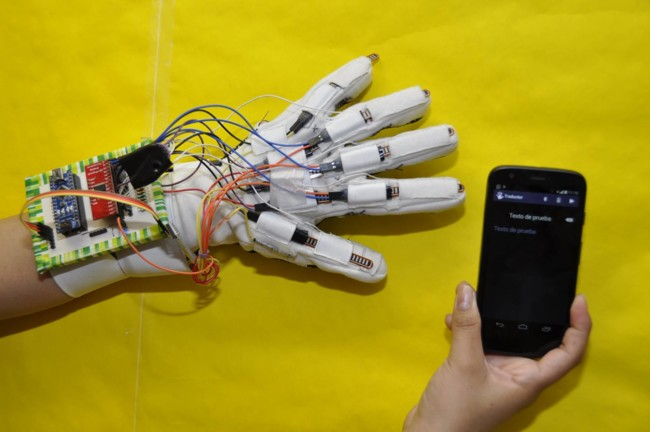
\includegraphics[scale = 0.5]{figures/guanteUPIITA}
			\caption{Traductor de lenguaje sordomudo mediante un guante con sensores y una aplicación móvil.}
			\label{guanteUPIITA}
		\end{figure}	

	\subsubsection*{Traductor del lenguaje de señas mexicano a texto usando FPGAS}

	En la escuela superior de cómputo del Instituto Politécnico Nacional se desarrolló como proyecto de titulación en el año 2003 un dispositivo que reconoce las características del lenguaje de señas mexicano y en tiempo real lo traduce como mensaje de texto. Lo hace mediante una cámara, el dispositivo permite tomar imágenes de las señas de la persona con problemas de audición, se reconocen y procesan en la FPGA para después traducir en forma de texto en tiempo real. El proyecto estuvo a cargo del Dr. Miguel Santiago Suárez Castañón. El prototipo está conformado por una cámara que capta las distintas señas, las traduce y en una pantalla las interpreta como un mensaje. Esto se realizó por medio de algoritmos de reconocimiento de patrones programados para interpretar las imágenes \cite{Yucatan2013} (Figura \ref{traductorESCOM})

		\begin{figure}[H]
			\centering
			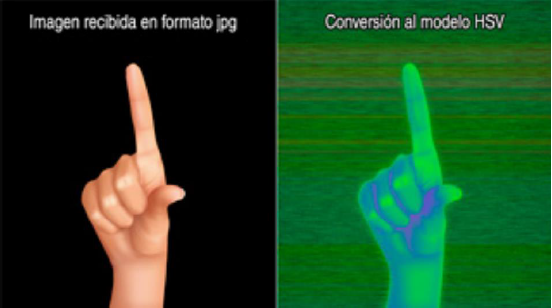
\includegraphics[scale = 0.5]{figures/traductorESCOM}
			\caption{Traductor del lenguaje de señas mexicano a texto usando FPGAS.}
			\label{traductorESCOM}
		\end{figure}

	\subsubsection*{Nacional}

	\subsubsection*{Intérprete de lenguaje de señas}

	Investigadores del Centro de Investigación y tecnología Aplicada (CITA) del Tecnológico de Monterrey, Campus Chihuahua apoyados por CONACYT, desarrollaron una tecnología que aplica la plataforma de videojuegos Kinect de Microsoft para traducir y dar voz a frases con el lenguaje de señas en español.

	Su objetivo es promover la integración social de las personas con discapacidad auditiva, así como mejorar la calidad de vida de los grupos desprotegidos mediante el uso de la tecnología.

	Principalmente el proyecto se basa en el procesamiento de imágenes para el reconocimiento de patrones. De esta forma cuando una persona esté frente al intérprete de lenguaje de señas y realice un movimiento con su cuerpo, el sistema reconoce y procesa los movimientos para posteriormente a través de un sistema de audio escuchar la traducción de los signos o señas.

	Se hace uso de la tecnología de Microsoft kinect Research Software Development Kit (SDK), además del software Language Integrated Query (LINQ), también de Microsoft, tecnología que les permitió implementar modelos conocidos del reconocimiento de imágenes con mayor sencillez \cite{Bustos2012} (Figura \ref{interpreteMICROSOFT}).

		\begin{figure}[H]
			\centering
			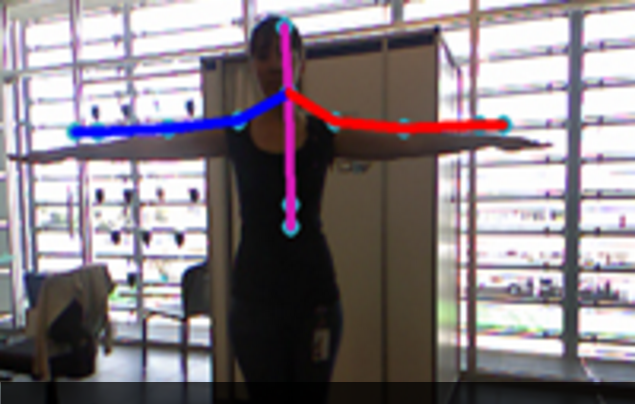
\includegraphics[scale = 0.5]{figures/lenguajeMicrosoft}
			\caption{Intérprete de lenguaje de señas.}
			\label{interpreteMICROSOFT}
		\end{figure}

	\subsubsection*{Internacional}

	\subsubsection*{Software convierte voz en lenguaje de señas para sordos}

	Investigadores de la Facultad de Ingeniería de la Universidad Nacional Autónoma de Honduras (UNAH) desarrollaron una plataforma en computadora capaz de convertir la voz en texto y éste en el lenguaje de señas hondureño para sordos (LESHO). Utiliza un avatar tridimensional que funciona como intérprete virtual, convirtiendo a LESHO el texto generado a partir de la voz del hablante.
	Su objetivo es hacer correr el software en cualquier navegador web y así evitar instalarlo en la computadora. El prototipo se mostró eficaz captando frases cortas en pruebas realizadas en junio del 2014 en los navegadores Chrome y Firefox.
	Se plantea probar el programa en las aulas de la UNAH antes de ampliar el uso, aunque aún falta la traducción de oraciones complejas ya que se requiere el análisis de la oración en español y su traducción al lenguaje de señas. Hasta el momento se han creado y suministrado al programa alrededor de 300 señas \cite{Oliveira2014}.

%	\subsubsection*{Sistema de traducción automática de voz o texto a LSE (Lengua de Signos Española)}
	
%	\subsubsection*{Hand Talk}
	
	\subsection{Del reconocimiento de voz}\label{sub:sr}

	En cuanto al ASR se han realizado diversos trabajos empleando diferentes técnicas de reconocimiento, así como también de extracción de características. En esta sección se muestran algunos trabajos enfocados al SR.

	\subsubsection*{Speech Recognition System Based on Short-term Cepstral Parameters, Feature Reduction Method and Artificial Neural Networks \cite{Nawel2016}}\label{sub:sota:Nawel2016}
	
	En este trabajo se desarrolla un ASR basado en parámetros cepstrales de términos cortos esto para identificar deficiencias de la voz como herramienta complementaria para otras técnicas médicas.
	Para esto utiliza y compara los resultados obtenidos al usar los coeficientes MFCC, su primera y segunda derivada, además para detectar las deficiencias se investiga el uso de LDA para mejorar la habilidad de discriminar del sistema. Además de evaluar el sistema en términos de exactitud, sensitividad, especificidad, precisión y área bajo la curva.
	
	Las características de los métodos y técnicas usadas son las siguientes:
	
	\begin{itemize}
	\item	Se ocupó la base de datos \textit{Saarbrucken Voice Database}, que es una colección de señales de voz con transtornos alemanes que contiene 2225 muestras de voz con una tasa de muestreo de 50 kHz y una resolución de 16 bits.
	\item	La extracción de características se hace por medio de MFCC y se calculan 13 coeficientes, su primera derivada y su segunda derivada. Para la optimización de características se emplea el análisis LDA.
	\item	La arquitectura de la red neuronal propuesta es de tres capas, la capa oculta contiene 250 neuronas a la cual se le aplica la función de activación \textit{sigmoid} y la capa de salida que contiene una neurona con función lineal.
	\item	El aprendizaje de la red neuronal es realizado basado en los algoritmos de regularización bayesiana.
	\item	El conjunto de datos se dividió, un 70\% para el entrenamiento y 30\% para la validación.
	\item	Las simulaciones fueron hechas en Matlab 2013a con Intel Core-i7, 2.20 GHzCPU y 4 GB de RAM.
	\end{itemize}
	
	Los resultados obtenidos muestran que el uso de características MFCC, deltas 1 y 2 y LDA tiene mejor resultado (87.82\% de exactitud) contra los 75.13\% haciéndo uso únicamente de MFCC. 
	
	%\subsubsection*{Phoneme Recognition Using Time-Delay Neural Networks \cite{ALEXANDER1989}}
	
	
	
	%\subsubsection*{Global Optimization of a Neural Network-Hidden Markov Model Hybrid \cite{Yosgua1992}}

	\subsubsection*{DEVELOPMENT OF ISOLATED SPEECH RECOGNITION SYSTEM FOR BANGLA WORDS \cite{A30}}\label{sub:sota:A30}
	
		En este trabajo se desarrolla un sistema de reconocimiento de palabras aisladas del idioma bengalí, para este sistema se destacan las siguientes características:
	
	\begin{itemize}
	\item	De 1 a 6 interlocutores.
	\item	Basado en palabras aisladas y en unidades de palabras (subwords).
	\item	El formato de archivo manejado es WAV.
	\item	Las palabras son agrupadas en 3 grupos diferentes de acuerdo al número de sílabas.
	\item	Para la extracción de características se usa MFCC.
	\item	El sistema de reconocimiento usado es la distancia euclidiana.
	\item	En total se tienen 600 palabras distintas.
	\item	Software utilizado es Turbo C
	\end{itemize}
	
	Las condiciones de las palabras grabadas son las siguientes:
	
	\begin{itemize}
	\item	Las muestras de voz fueron grabadas en un laboratorio insonorizado.
	\item	Se usaron micrófonos de proximidad.
	\item	Tarjetas de audio y software de grabación de alta calidad.
	\item	Las palabras se grabaron a una tasa de muestreo de 8 kHz y se codificaron con PCM de 8 bits.
	\end{itemize}
	
	Algunas características del procesamiento son:
	
	\begin{itemize}
	\item	Segmentación de 16 a 32 ms.
	\item	Para el preénfasis se utilizó la siguiente ecuación
		\begin{equation}\label{eq:xxx}
			y(n)=s(n)-C\cdot s(n-1)
		\end{equation}
		Con valores de $C=0.9 - 1.0$
	\item	Se aplicó la ventana Hamming
	\item	Método de reconocimiento aplicado fue la distancia euclidiana.
	\end{itemize}
	
	Las tasas de reconocimiento obtenidas van de 79.11\% para 6 interlocutores con 3600 palabras en la base de datos a 96\% para un interlocutor y 600 palabras en la base de datos.
	
	\subsubsection*{Continuous Bangla Speech Segmentation using Short-term Speech Features Extraction Approaches \cite{A31}}\label{sub:sota:A31}
	
	Para este trabajo presenta la segmentación de palabras del idioma Bangla usando enfoques de extracción de características.
	
	Las características del dominio del tiempo usadas son la energía y la tasa de cruces por cero de una señal de tiempo corto, por otro lado, en el dominio de la frecuencia se hace uso del centroide espectral y el flujo espectral.
	
	Algunas características de este trabajo son:
	
	\begin{itemize}
	\item	Se utiliza el criterio de umbral dinámico para detectar los bordes de la palabra.
	\item	El interlocutor es un hombre y las muestras se graban a una frecuencia de muestreo de 16 kHz y el tamaño de la muestra es de 8 bits.
	\item	Tamaño del segmento de 50 ms y un traslape de 10 ms, además de usar una ventana rectangular.
	\item	El proceso se lleva a cabo en Matlab 7.12.0.
	\item	El proceso es el siguiente: Adquisición del habla, pre-procesamiento de la señal, extracción de características, cálculo del histograma, umbral dinámico y post-procesamiento.
	\end{itemize}
	
	La tasa de segmentación presentada es de 96.25\%.
	
	\subsubsection*{An Efficient Noise-Robust Automatic Speech Recognition System using Artificial Neural Networks \cite{A3}}\label{sub:sota:A3}
	
	En este trabajo se presenta una técnica de reconocimiento para señales con ruido, se trabaja con 65 palabras diferentes y con una relación señal a ruido de hasta -5dB, se utilizaron los coeficientes MFCC como características para el reconocimiento de voz, la red neuronal empleada es Backpropagation y diversos algoritmos de entrenamiento fueron empleados, los cuales son:
	
	\begin{itemize}
	\item	Polak-Ribiére Conjugate Gradient (CGP).
	\item	Resilient Backpropagation (RP).
	\item	Conjugate Gradient with Powell/Beale Restarts (CGB).
	\item	Scaled Conjugate Gradient backpropagation (SCG).
	\end{itemize}
	
	Las señales de voz utilizadas fueron sintetizadas para obtenerlas lo más limpias posible con un modelo basado en HMM, con una tasa de muestreo de 48000 muestras por segundo con un modelo femenino. Cada palabra se sintetizó 20 veces variando el tono, duración, sonidos sordos y sonoros obteniendo un total de 1300 muestras diferentes. Estas muestras se contaminan con ruido gaussiano reduciendo la SNR de 5dB a -3 dB siendo estas señales las entradas al sistema.
	
	Por otro lado se hace la extracción y compresión de características usando los coeficientes MFCC y para cada vector se calculo su media y varianza, el autor menciona que no utiliza la compresión \textit{K-means} debido a su complejidad y consumo de tiempo.
	
	La estructura de la red neuronal está dada por la entrada la cual toma el vector de características compreso, una capa oculta con función de activación \textit{sigmoid} y la capa de salida con la función de activación \textit{softmax}.
	
	Los resultados presentan que para una longitud de vector de entrada de 20, SNR de -5dB y 30 palabras diferentes con la versión de la red neuronal \textit{Pattern Recognition Network} da un resultado de 94.5\% de exactitud de reconocimiento, para una longitud de 40 del vector de características el mejor resultado es de 98.7\% de exactitud con el algoritmo de entrenamiento SCG.
	
	Finalmente se selecciona la versión de red \textit{Pattern Recognition} y algoritmo de entrenamiento SCG y se hacen pruebas con diferente número de neuronas de la capa oculta y el mejor resultado para un SNR de -3dB y longitud de vector de 40 con 99.6\% son 40 neuronas y para un SNR de -5dB se tuvo el mejor resultado de 99.4\% con 20 neuronas.
	
	\subsubsection*{Combination of Vector Quantization and Hidden Markov Models for Arabic Speech Recognition \cite{A6}}\label{sub:sota:A6}
	
	En este trabajo se presenta el reconocimiento de voz para el árabe usando cuantización vectorial y HMM.
	
	Algunas características de este trabajo son:
	
	\begin{itemize}
	\item	Tasa de muestreo de 11025 Hz
	\item	La etapa de preénfasis se aplicó de acuerdo a la siguiente ecuación
		\begin{equation}\label{eq:xxx}
			\hat{s}(n)=s(n)-a\cdot s(n-1)
		\end{equation}
		Con valor de $a=0.8$
	\item	Los segmentos son de 45 ms espaciadas por 15 ms y un traslape de 30 ms.
	\item	Se aplica la ventana de Hamming
	\item	Para las características se hace un análisis LPC/Cepstral
	\item	Se utilizan los coeficientes Delta Cepstrum
	\item	Se aplica cuantización vectorial
	\item	Las palabras corresponden a los 10 dígitos con 30 interlocutores de entrenamiento y cada uno hace 3 repeticiones por palabra.
	\end{itemize}
	
	En los resultados se muestran dos grupos, los interlocutores que participan en el entrenamiento y los que no. En el primero grupo son los 30 interlocutores y se tiene una tasa de reconocimiento de 95\% y en el segundo grupo se tienen 10 interlocutores con una tasa de reconocimiento de 91\%.
	
	\subsubsection*{COMBINING FUZZY VECTOR QUANTIZATION AND NEURAL NETWORK CLASSIFICATION FOR ROBUST ISOLATED WORD SPEECH RECOGNITION \cite{A7}}\label{sub:sota:A7}
	
	En este trabajo se presenta la combinación de FVQ y NN para llevar a cabo el reconocimiento de voz de palabras aisladas, para esto se emplea una red neuronal multicapa perceptron (MLP) y se compara con FVQ/HMM, agregando ruido blanco o \textit{car noise}.
	
	Las características de la señal de voz son:
	
	\begin{itemize}
	\item	Entrada con banda limitada a 3.6 kHz.
	\item	Tasa de muestreo a 8 kHz con un tamaño de muestra de 16 bits.
	\item	Los segmentos tienen una longitud de 20 ms y un traslape de 10 ms, y cada segmento se analiza con LPC produciendo un vector de 16 LSP y cada conjunto de coeficientes LSP se cuantiza vectorialmente.
	\item	En total se tienen 1040 palabras con 8 interlocutores ingleses, 5 hombres y 3 mujeres, cada interlocutor dio 13 repeticiones de los diez dígitos de las cuales 10 fueron usadas para entrenamiento y 3 para evaluar el desempeño.
	\end{itemize}
	
	Los resultados obtenidos con una SNR de 20dB a 35dB son del 41\% a 95.42\% (el mayor usando FVQ/MLP con 20 nodos ocultos), por otro lado el uso de FVQ/HMM a 35dB de SNR dio como mejor resultado 92.67\% de exactitud de reconocimiento. Estas pruebas se realizaron con ruido blanco.
	
	Para el uso de \textit{car noise} el mejor resultado fue a 35dB de SNR, con el uso de FVQ/HMM se obtuvo una exactitud de 95.83\% y 98.33\% usando FVQ/MLP con  10 nodos ocultos.
	
	\subsubsection*{Combining Neural Network Classification with Fuzzy Vector Quantization and Hidden Markov Models for Robust Isolated Word Speech Recognition \cite{A8}}\label{sub:sota:A8}
	
	En este trabajo se presenta un esquema FVQ/HMM/MLP. Dos conjuntos de entradas fueron usadas en ese experimento, el primer conjunto compuesto de los diez dígitos en inglés, mientras que el segundo conjunto empleó las 26 letras del inglés.
	
	Los resultados obtenidos muestran que se tiene un mejor desempeño de reconocimiento bajo condiciones de ruido que los esquemas FVQ/HMM y FVQ/MLP, el sistema obtuvo una tasa de reconocimiento del 98.33\% a 30 dB de SNR y 90\% a 20dB de SNR cuando se opera en el primer conjunto de palabras.
	
	\subsubsection*{English speech recognition method based on Hidden Markov model \cite{A13}}\label{sub:sota:A13}
	
	En este trabajo se presenta el uso de HMM para reconocimiento de voz en inglés, haciendo pruebas en diferentes ambientes de ruido, además de presentar una mejora a la técnica de HMM.
	
	Para esto se utiliza la base de datos \textit{Aurora 2 English database} la cual se basa en la base de datos \textit{TIDIGITS} submuestreada a 8 kHz y agrega diferentes señales de ruido. La base de datos \textit{TIDIGITS} tiene 326 interlocutores (111 hombres, 114 mujeres, 50 niños y 51 niñas), cada uno pronuncia 77 secuencias de dígitos, para las grabaciones se usó un micrófono \textit{Electro-Voice RE-16 Dynamic Cardiod}, muestreado a 20 kHz.
	
	La mejora al método de HMM es la adición de una capa oculta para representar la evolución del estado de transición.
	
	Los resultados obtenidos con la técnica HMM y HMM mejorada se muestran en la Tabla \ref{tb:hmm}:
	
	% Please add the following required packages to your document preamble:
	% \usepackage{multirow}
	\begin{table}[H]
	\centering
	\caption{Promedio de precisión de reconocimiento}
	\label{tb:hmm}
	\begin{tabular}{|l|l|l|}
	\hline
	\multicolumn{1}{|c|}{\multirow{2}{*}{Ambiente}} & \multicolumn{2}{l|}{Precisión de reconocimiento} \\ \cline{2-3} 
	\multicolumn{1}{|c|}{}                          & HMM                  & HMM mejorado              \\ \hline
	Subway                                          & 44.87\%              & 49.98\%                   \\ \hline
	Babble                                          & 45.72\%              & 49.25\%                   \\ \hline
	Car                                             & 52.79\%              & 57.95\%                   \\ \hline
	Exhibition hall                                 & 55.27\%              & 59.84\%                   \\ \hline
	\end{tabular}
	\end{table}


	A continuación se presenta la tabal comparativa de los artículos presentados.
	
	\newpage
	 \begin{landscape}
	\begin{table}[]
\centering
\caption{Tabla comparativa de técnicas de reconocimiento de voz}
\label{tb:comparativaSOA}
\scalebox{0.9}{
\begin{tabular}{|l|l|l|l|l|}
\hline
Trabajo  & Pre-procesamiento                                                                                                                                                        & \begin{tabular}[c]{@{}l@{}}Técnica de\\ reconocimiento\end{tabular}                                                               & Características                                                                                                                                                                                                      & Resultados                                                                                                       \\ \hline
{[}11{]} & \begin{tabular}[c]{@{}l@{}}MFCC (13 coeficientes)\\ primera y segunda derivada\end{tabular}                                                                              & \begin{tabular}[c]{@{}l@{}}Red neuronal,\\ \\ aprendizaje basado en\\ algoritmos de regularización\\ bayesiana\end{tabular}       & \begin{tabular}[c]{@{}l@{}}Base de datos \\ \textit\{Saarbrucken Voice Database\}\\ Tasa de muestreo a 50 kHz\\ y resolución de 16 bits\end{tabular}                                                                 & \begin{tabular}[c]{@{}l@{}}Uso de MFCC, deltas 1 y 2\\ y análisis LDA, exactitud\\ de 87.82\%\end{tabular}       \\ \hline
{[}12{]} & \begin{tabular}[c]{@{}l@{}}Extracción de características\\ MFCC\\ Ventana Hamming\\ Segmentación de 16 a 32 ms\end{tabular}                                              & Distancia euclidiana                                                                                                              & \begin{tabular}[c]{@{}l@{}}1 a 6 interlocutores\\ Tarjetas de audio y software de \\ alta calidad\\ 600 palabras distintas\\ Tasa de muestreo a 8 kHz\\ y resolución de 8 bits\end{tabular}                          & \begin{tabular}[c]{@{}l@{}}Resultados de 96\% con\\ 1 interlocutor y 79.11\% con\\ 6 interlocutires\end{tabular} \\ \hline
{[}13{]} & \begin{tabular}[c]{@{}l@{}}Segmentación de palabras.\\ Segmentos de 50 ms y \\ traslape de 10 ms\end{tabular}                                                            & \begin{tabular}[c]{@{}l@{}}Segmentación con umbral\\ dinámico\end{tabular}                                                        & \begin{tabular}[c]{@{}l@{}}Uso de 4 características\\ energía\\ tasa de cruces por cero\\ flujo espectral\\ y centroide espectral\end{tabular}                                                                       & Resultados de 96.25\%                                                                                            \\ \hline
{[}14{]} & \begin{tabular}[c]{@{}l@{}}Extracción de características\\ MFCC, compresión con\\ media y varianza\end{tabular}                                                          & \begin{tabular}[c]{@{}l@{}}Red neuronal backpropagation\\ con algoritmos de \\ entrenamiento:\\ CGP\\ RP\\ CGB\\ SCG\end{tabular} & \begin{tabular}[c]{@{}l@{}}Mejores resultados con \\ \textit\{Pattern Recognition Network\}\\ 65 palabras diferentes\\ con 20 repeticiones cada una,\\ variando tono, duración, etc.\\ SNR de -5 a 5 dB\end{tabular} & \begin{tabular}[c]{@{}l@{}}Para SNR de -5dB se tiene\\ resultado de 99.4\%\end{tabular}                          \\ \hline
{[}15{]} & \begin{tabular}[c]{@{}l@{}}Análisis LPC y delta cepstrum\\ Ventana de Hamming\\ Tasa de muestreo de 11025 kHz\\ Segmentos de 45 ms con \\ traslape de 30 ms\end{tabular} & \begin{tabular}[c]{@{}l@{}}HMM con cuantización \\ vectorial\end{tabular}                                                         & \begin{tabular}[c]{@{}l@{}}30 interlocutores y palabras\\ correspondientes a los 10 dígitos\\ cada uno hace 3 repeticiones de cada\\ palabra\end{tabular}                                                            & \begin{tabular}[c]{@{}l@{}}Tasa de reconocimiento de \\ 91\% a 95\%\end{tabular}                                 \\ \hline
{[}16{]} & \begin{tabular}[c]{@{}l@{}}Análisis LPC a 16 coeficientes\\ Segmentos de 20 ms y \\ traslape de 10 ms\end{tabular}                                                       & \begin{tabular}[c]{@{}l@{}}FVQ/MLP\\ FVQ/HMM\end{tabular}                                                                         & \begin{tabular}[c]{@{}l@{}}1040 palabras\\ 8 interlocutores\\ 13 repeticiones de los 10 dígitos\\ SNR de 20dB a 35dB\end{tabular}                                                                                    & \begin{tabular}[c]{@{}l@{}}Mejor resultado con \\ FVQ/MLP de 98.33\% a 35 dB\\ de SNR\end{tabular}               \\ \hline
{[}17{]} & --                                                                                                                                                                       & FVQ/HMM/MLP                                                                                                                       & 10 dígitos en inglés                                                                                                                                                                                                 & \begin{tabular}[c]{@{}l@{}}Reconocimiento de 98.33\%\\ a 30dB de SNR\end{tabular}                                \\ \hline
{[}18{]} & Muestreo de 8 kHz                                                                                                                                                        & HMM y HMM mejorada                                                                                                                & \begin{tabular}[c]{@{}l@{}}Base de datos \\ \textit\{Aurora 2 English database\}\end{tabular}                                                                                                                        & Tabla                                                                                                            \\ \hline
\end{tabular}}
\end{table}

\end{landscape}
	
%	\subsection{De reconocimiento}
	
%	Diferentes implementaciones de un ASR se han llevado a cabo con diferentes técnicas, algoritmos y herramientas, a continuación se mencionan algunos resultados obtenidos.
	
%	En \cite{A1} se define ASR (Automatic speech recognition) como la transcripción independiente, computarizada del lenguaje hablado en texto legible en tiempo real.
	
%	Aquí se mencionan los diferentes métodos usados para ASR, dentro de los cuales destaca el uso de HMM ya que la voz puede visualizarse como una señal estacionaria pieza por pieza o una señal estacionaria de corto tiempo. También menciona que el uso de redes neuronales puede ser eficiente en SR pero no en tareas de reconocimiento continuo, debido a su falta de capacidad para modelar dependencias temporales.
	
%	Uno de los componentes principales del ASR es la extracción de características ya que este proceso usa la información más relevante de la señal de voz y ayuda a distinguir entre diferentes unidades lingüísticas y elimina ruido externo, perturbaciones y emociones. Las técnicas de extracción más comunes  son MFCC, LPC, LPCC, de las cuales \cite{A1} menciona que la técnica MFCC ha sido comprobada como el estado del arte en cuanto a extracción de características desde que se basa en el sistema de audición humana y trabaja sobre una escala de frecuencias llamada \textit{Mel}. Para lenguajes como el inglés, chino, japonés e incluso el hindi se han tenido eperimentalmente resultados del 80\% de eficiencia contral el 60\% que tienen LPC y LPCC.
	

	
	

\section{Marco teórico}

En esta sección se muestran las bases sobre las que se sustenta el presente trabajo, se abordan los temas referentes al lenguaje de señas mexicano, así como el procesamiento involucrado en el reconocimiento de voz como es la adquisición de la señal de voz, su procesamiento y las técnicas a emplear para la detección de palabras, así como también la base de datos utilizada y las comunicaciones requeridas.

\subsection {Estructura básica de la oración}

Para definir las palabras y oraciones que serán empleadas para realizar la detección e interpretación a lenguaje de señas, se plantea el estudio de la estructura básica de la oración para el LSM ya que ésta presenta diferencias con la oración del idioma español que conocemos, esto con el fin de poder analizar las oraciones y determinar su equivalente en LSM.

Para empezar, debemos tomar en cuenta las particularidades que presentan las lenguas viso gestuales como el LSM, la tarea de describir la sintaxis que presentan las lenguas, ya sean orales o de señas, se debe reflexionar sobre dos nociones fundamentales: la proposición y la oración.

La proposición hace referencia a un proceso interno en el cual cada persona combina y manipula conceptos con el fin de comunicarse. Así, en una proposición se involucran una o dos entidades conceptuales con una relación, actividad o propiedad que les concierne. La oración es la expresión lingüística de una proposición.

Ahora bien, la oración básica o simple se caracteriza por ser la unidad sintáctica formada por la unión de un predicado y su sujeto.

El sujeto está constituido por una frase nominal que puede ser un nombre (con o sin determinantes, o con modificadores), un pronombre, o una oración, o bien puede estar ausente.

Por otra parte, el predicado es lo que se dice del sujeto, el verbo es el núcleo o palabra esencial de esta unidad sintáctica. En la LSM, así como en otras lenguas de señas, la clase de verbos (llanos y demostrativos) puede influir en el orden de constituyentes que presenta. Aunque de manera general se puede decir que en la LSM el orden de constituyentes que se observa en la mayoría de las construcciones gramaticales es Sujeto-Verbo-Objeto (SVO), se presentan las variaciones OSV, VOS, VSO, OVS y SOV, según el tipo de verbo que se utilice, así como por situaciones pragmáticas y semánticas. Por tanto, la LSM es una lengua cuyo orden responde no sólo a los principios que regulan las relaciones gramaticales sino además a aspectos semánticos y pragmáticos. \cite{Aldrete2008}

El LSM al igual que cualquier otro idioma se sustenta a base de reglas gramaticales para la estructuración de oraciones. La regla principal para el ordenamiento de frases es la siguiente.

\begin{centering}

Tiempo – Lugar – Sujeto – Objeto – Verbo

\end{centering}

\begin{itemize}

\item	Tiempo: establece el momento en que sucede la acción
\begin{itemize}
\item	Ejemplos: Antes, ahora, hoy, en el futuro, mientras, etc.
\end{itemize}
\item	Lugar: el sitio donde ocurre la acción
\begin{itemize}
\item	Ejemplos: Aquí, nombres de ciudades, países, etc.
\end{itemize}
\item	Objeto: Las personas o cosas que reciben la acción del sujeto
\begin{itemize}
\item	El objeto se indica antes del sujeto y debe ubicarse en un espacio.
\end{itemize}
\item	Sujeto: Las personas o coas que realizan la acción
\begin{itemize}
\item	El sujeto se indica inmediatamente antes de la acción que va a realizar y debe ubicarse en un espacio.
\end{itemize}
\item	Verbo: la acción
\begin{itemize}
\item	Ejemplos: Correr, hacer, platicar, seguir, etc.
\end{itemize}
\item	Preguntas: La palabra interrogante (cuándo, cómo, dónde) va al final, acompañada de la expresión facial.

\end{itemize}

Tomando en cuenta este último punto , si deseamos generalizar más la estructura obtenemos:

\begin{centering}
Tiempo – Lugar – Sujeto – Objeto – Verbo – Pregunta
\end{centering}

\subsection{¿Cómo formar oraciones?}

De acuerdo a la estructura anterior se darán unos ejemplos de cómo formar oraciones en LSM a partir de una en español.

\begin{itemize}

\item	Formar oraciones

\begin{itemize}
\item	Español: Fui rápido al mercado.
\begin{itemize}
\item	LSM: Pasado mercado yo ir rápido.
\end{itemize}
\item	Español: Yo jugué futbol el mes pasado en Cuernavaca.
\begin{itemize}
\item	LSM: Mes pasado Cuernavaca yo futbol jugar.
\end{itemize}
\item	Español: Próximo diciembre me iré de vacaciones a Acapulco.
\begin{itemize}
\item	Próximo diciembre Acapulco yo vacaciones ir.
\end{itemize}
\end{itemize}

\item	Oraciones interrogativas

\begin{itemize}
\item	Español: ¿Tienes hermanos?
\begin{itemize}
\item	LSM: ¿Tú hermanos tener cuántos?
\end{itemize}
\item	Español: ¿Qué quieres comer?
\begin{itemize}
\item	LSM: ¿Tú comer que significa?
\end{itemize}
\item	Español: ¿Cuáles son tus hermanos?
\begin{itemize}
\item	LSM: ¿Ellos hermanos tuyos cuáles?
\end{itemize}
\end{itemize}

\item	Oraciones y señas negativas

\begin{itemize}
\item	Español: Yo quiero un helado de chocolate, no de fresa.
\begin{itemize}
\item	LSM: Yo helado chocolate querer no fresa.
\end{itemize}
\item	Español: No me fui de vacaciones.
\begin{itemize}
\item	LSM: Agosto pasado yo vacaciones ir nada.
\end{itemize}
\item	Español: El pozole de la abuela no me gusta.
\begin{itemize}
\item	LSM: Yo pozole abuela no me gusta.
\end{itemize}
\end{itemize}

\end{itemize}

\subsection{Características de la señal de voz}

En esta sección se estudian las características de la señal de voz en el dominio del tiempo y la frecuencia, así como también se hace el análisis estadístico de la voz.

\subsubsection{Tiempo}

Básicamente de acuerdo al estado de la fuente de producción de voz podemos clasificar en tres estados a la señal de voz. Estos son: silencio (SL), en el que no hay voz; voz sorda (SR), en el que las cuerdas vocales no vibran, y voz sonora (SN) en el que las cuerdas vocales vibran dando lugar a una señal casi periódica. \cite{Mesa}

Como ejemplo en la Figura \ref{fig:sixOnda} se muestra la gráfica de la señal de voz correspondiente a la palabra six pronunciada por un hombre, el eje horizontal representa el tiempo en segundos y el eje vertical representa la amplitud de la señal. Inicialmente tenemos silencio hasta los 0.58 segundos, los siguientes 120 ms observamos que la señal es sorda correspondiente al fonema /s/ al cual le sigue un abrupto incremento de energía en un intervalo de 120 ms en el que la señal es sonora, perteneciente al fonema /I/, al que le sigue un silencio intrasilábico de 80 ms y finalmente otro intervalo de voz sorda, correspondientes a los fonemas /k/ y /s/, de alrededor de 230 ms seguidos de un silencio.

\begin{figure}[H]
	\centering
	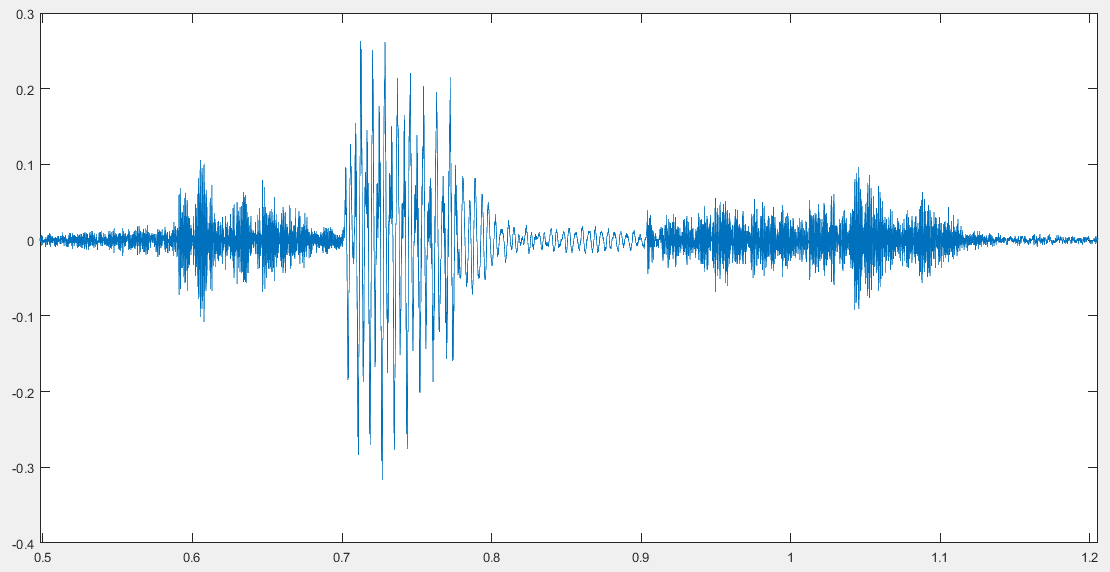
\includegraphics[width=1\linewidth]{figures/sixOnda}
	\caption{Forma de onda de la palabra ''six''}
	\label{fig:sixOnda}
\end{figure}

Una característica de la señal de voz que obtenemos en el dominio del tiempo es la energía de la señal, la cual es la suma del cuadrado del módulo de la señal o un intervalo de ésta, en el caso de la señal de voz es la suma del cuadrado de las amplitudes y queda definida de la siguiente forma:
		
\begin{equation}\label{eq:energia}
	E = \sum_{n=-\infty}^{\infty}{|x(n)|^2}
%	y = f \left[ \left( \sum_{i=1}^{N}\omega_i*x\left(n-i\right)\right)-b	\right]
\end{equation}		

Donde:
\\$E->$ energía de la señal.
\\$x->$ señal de voz.


La energía nos puede ser de utilidad para determinar si la señal de voz es sonora o sorda, de la Figura \ref{fig:sixOnda} podemos observar que la forma de onda del fonema /s/ tiene menor amplitud que la forma de onda correspondiente al fonema /I/, es evidente que, si tomamos un intervalo del mismo número de muestras para cada fonema, el valor de energía para esos intervalos será mayor para el fonema /I/ que representa una señal sonora. Esta técnica para determinar la clasificación de la señal de voz no es efectiva, ya que la señal sorda y el silencio se equiparán en amplitud lo cual causaría errores de clasificación.

El tono es otra característica de la voz, en \cite{MediaRadio} se dice que el tono es la impresión que nos produce la frecuencia de vibración a la que se manifiesta una determinada onda sonora, para el caso de la producción de la voz, la marca de tono (grave o agudo) viene dada por la cantidad de movimiento que se produce en las cuerdas vocales al emitirla, es decir, el número de vibraciones que en ellas tiene lugar. Dada la definición anterior, es posible determinar el tono de la señal de voz a partir de su representación en el tiempo.

\subsubsection{Frecuencia}

El concepto de formante es de gran importancia en cualquier tema relacionado con el análisis de la señal de voz, pues en ellos (en su distribución y estructura) está concentrada la mayor parte de la información psicoacústica transportada por la señal de voz que permite la comprensión del mensaje, éstos son picos en el espectro de voz consecuencia de las resonancias en el tracto vocal. \cite{Mesa}

Las frecuencias de resonancia son características esenciales de los formantes, las frecuencias de los tres primeros formantes pueden constituir un sistema de referencia absoluto para los sonidos vocálicos, en el que las distintas vocales quedan representadas de forma relativamente independiente del locutor.

El domino frecuencial nos permite conocer la estructura de los formantes, la representación espectral es una técnica que nos ayuda a conocer las características frecuenciales relevantes de la señal de voz. En la Figura \ref{fig:espectroSonora} (tomada de \cite{Mesa}) se aprecia el espectro correspondiente a una señal genérica de voz sonora, gracias a esta representación podemos observar características tales como los formantes o la frecuencia fundamental y sus armónicos. La frecuencia fundamental es la frecuencia de vibración de las cuerdas vocales. Para los hombres esta frecuencia está entre 100-125 Hz dependiendo de la edad y para las mujeres es de 200-250Hz. En la figura podemos distinguir tres formantes, F1, F2 y F3, así como la frecuencia fundamental, F0.

\begin{figure}[H]
	\centering
	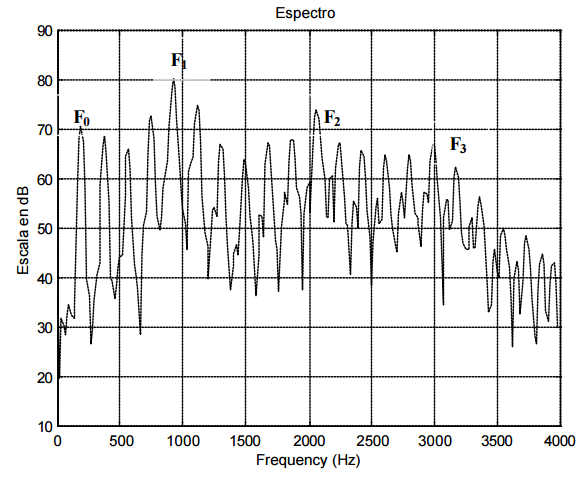
\includegraphics[width=0.8\linewidth]{figures/espectroSonora}
	\caption{Espectro de una señal sonora}
	\label{fig:espectroSonora}
\end{figure}

Una forma alterna de caracterizar la señal de voz y representar su información asociada es por medio de una representación conjunta de tiempo y frecuencia. El espectrograma es una representación tiempo frecuencia tridimensional en la que se muestra la intensidad de la voz y su evolución temporal en diferentes bandas frecuenciales.

En el espectrograma de banda ancha los sucesos temporales están resueltos con gran precisión mostrando, por ejemplo, barras verticales durante los intervalos sonoros asociados a los instantes de cierre glótico. La resolución frecuencial, a diferencia de la temporal, es pobre. Por el contrario, el espectrograma de banda estrecha tiene peor resolución temporal pero una mejor resolución frecuencial. En éste, los armónicos de la frecuencia fundamental están bien resueltos y definidos como líneas casi horizontales.

En la Figura \ref{fig:spectrogram} se muestra la forma de onda de la señal de voz, la magnitud del espectro en frecuencia y el espectrograma, en el cual se muestra la evolución de la potencia de los componentes frecuenciales a través del tiempo, podemos observar cómo aumenta la potencia de los componentes frecuenciales en el periodo de tiempo en que la amplitud de la forma de onda aumenta.

\begin{figure}[H]
	\centering
	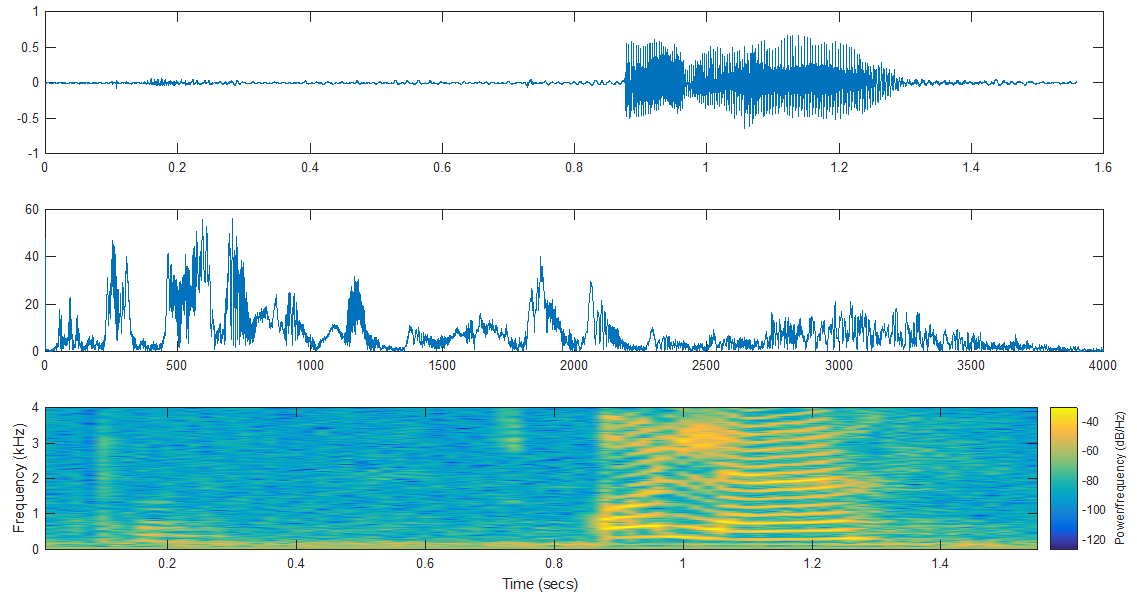
\includegraphics[width=1\linewidth]{figures/spectrogram}
	\caption{Espectrograma de la señal de voz}
	\label{fig:spectrogram}
\end{figure}

\subsubsection{Estadístico}

Algunos aspectos a estudiar sobre la naturaleza estadística de la voz son: función de densidad de probabilidad (FDP), estacionariedad y ergodicidad.

La FDP se puede estimar mediante un histograma de las amplitudes sobre un número suficientemente grande y representativo de muestras de señal. La estadística de la voz queda bien representada por una distribución laplaciana o, en mejor medida, por una distribución gamma.

En \cite{Mesa} se dice que en la mayoría de técnicas de extracción de características es conveniente hacer la suposición que la voz es un proceso estocástico ergódico y aunque resulta un modelo simplista, los resultados obtenidos en la práctica justifican su validez. Un ejemplo es que la autocorrelación de un proceso ergódico puede ser obtenida mediante la estimación de un promedio temporal conveniente. La estimación se tiene que hacer con un segmente suficientemente largo, aunque finito, de la señal. La validez del modelo ergódico está ligada a la suposición de la estacionariedad. La voz es un proceso estacionario o no según la longitud del intervalo de observación. La señal de voz es una señal de evolución lenta, cuando se observa en intervalos de tiempo suficientemente cortos (típicamente, entre 20 y 60 ms), sus características son prácticamente estacionarias. Se dice entonces que se trata de una señal casi estacionaria. Vista en intervalos largos (del orden de un cuarto de segundo o más) las características de la voz cambian para reflejar los diferentes sonidos que se están pronunciando, dando lugar a una señal no estacionaria. Por lo tanto, la validez de ergodicidad ha de entenderse en intervalos donde sea cierto que la señal es estacionaria.

En los sistemas de reconocimiento, la extracción de características se hace en tramas de la señal, de modo que podamos suponer estacionariedad y ergodicidad.

\subsection{Producción de la voz}

La voz humana es producida en la laringe, cuya parte esencial, la glotis, constituye el verdadero órgano de fonación humano. El aire procedente de los pulmones, es forzado durante la espiración a través de la glotis, haciendo vibrar los dos pares de cuerdas vocales, que se asemejan a dos lengüetas dobles membranáceas. Las cavidades de la cabeza, relacionadas con el sistema respiratorio y nasofaríngeo, actúan como resonadores. \cite{GrupodeAcustica2002}

El sistema vocal humano puede dividirse en tres partes:

\begin{itemize}
\item	Aparato respiratorio: donde se almacena y circula el aire. Nariz, pulmones, tráquea, diafragma.
\item	Aparato de fonación: donde el aire se convierte en sonido. Laringe y cuerdas vocales.
\item	Aparato resonador: donde el sonido adquiere sus cualidades de timbre que caracterizan cada voz. Cavidad bucal, faringe, paladar óseo, senos maxilares y frontales.
\end{itemize}

\begin{figure}[H]
	\centering
	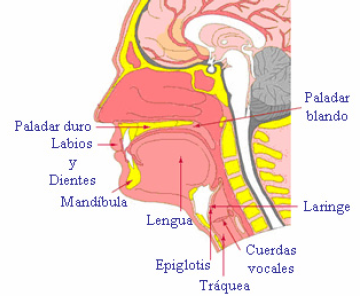
\includegraphics[width=0.6\linewidth]{figures/cavidadBucal}
	\caption{Cavidad bucal}
	\label{fig:cavidadBucal}
\end{figure}

De acuerdo al comportamiento de la cavidad bucal y la configuración de los órganos que participan en la generación de la voz, la señal generada puede clasificarse en dos tipos:

\begin{itemize}
\item	Señal sonora: se genera por la acción de las cuerdas vocales, las cuales se abren y cierran modificando el área de la tráquea y produciendo un tren de impulsos cuasi-periódicos. El período o frecuencia fundamental de este tren de impulsos se conoce con el nombre de pitch, y su valor está comprendido entre 50 y 400 Hz para los hombres y es superior en mujeres y niños. \cite{Alonso1999}
\item	Señal no sonora: el aire fluye libremente hasta alcanzar el tracto vocal al permanecer abiertas las cuerdas vocales, ésta presenta una estructura ruidosa tanto en el dominio del tiempo como en el de la frecuencia, no teniéndose formantes. Además, la energía de la señal es mucho menor que la de los sonidos sonoros. \cite{Alonso1999}
\end{itemize}

El tracto vocal actúa como una cavidad resonante para los sonidos sonoros, estando centradas las frecuencias de resonancia para la mayoría de la gente en 500 Hz y sus armónicos pares. Esta resonancia produce grandes picos en el espectro resultante, a los cuales se les llama formantes. Además, la señal tiene una naturaleza paso-baja y a partir de unos 4 KHz comienza a predominar el ruido.

Modelar el proceso de generación de la voz es útil en muchas aplicaciones, como la extracción de ciertos parámetros que permiten identificarla, ya que el tracto vocal se representa mediante un filtro que varía en el tiempo, dependiendo de la acción que se realiza al pronunciar una palabra. Si se obtienen dichos coeficientes, se tiene, por lo tanto, características de la señal de voz que nos permitirán identificarla.

En la Figura \ref{fig:modeloSimplificado} se muestra el modelo simplificado de la producción de la voz, el filtro que modela el tracto vocal tiene dos posibilidades de entrada, que dependerá de si la señal es sonora o no. Para señales sonoras, la excitación será un tren de impulsos de frecuencia controlada (pitch), mientras que para las señales no sonoras la excitación será ruido blanco. \cite{SalcedoCherubini2006}

\begin{figure}[H]
	\centering
	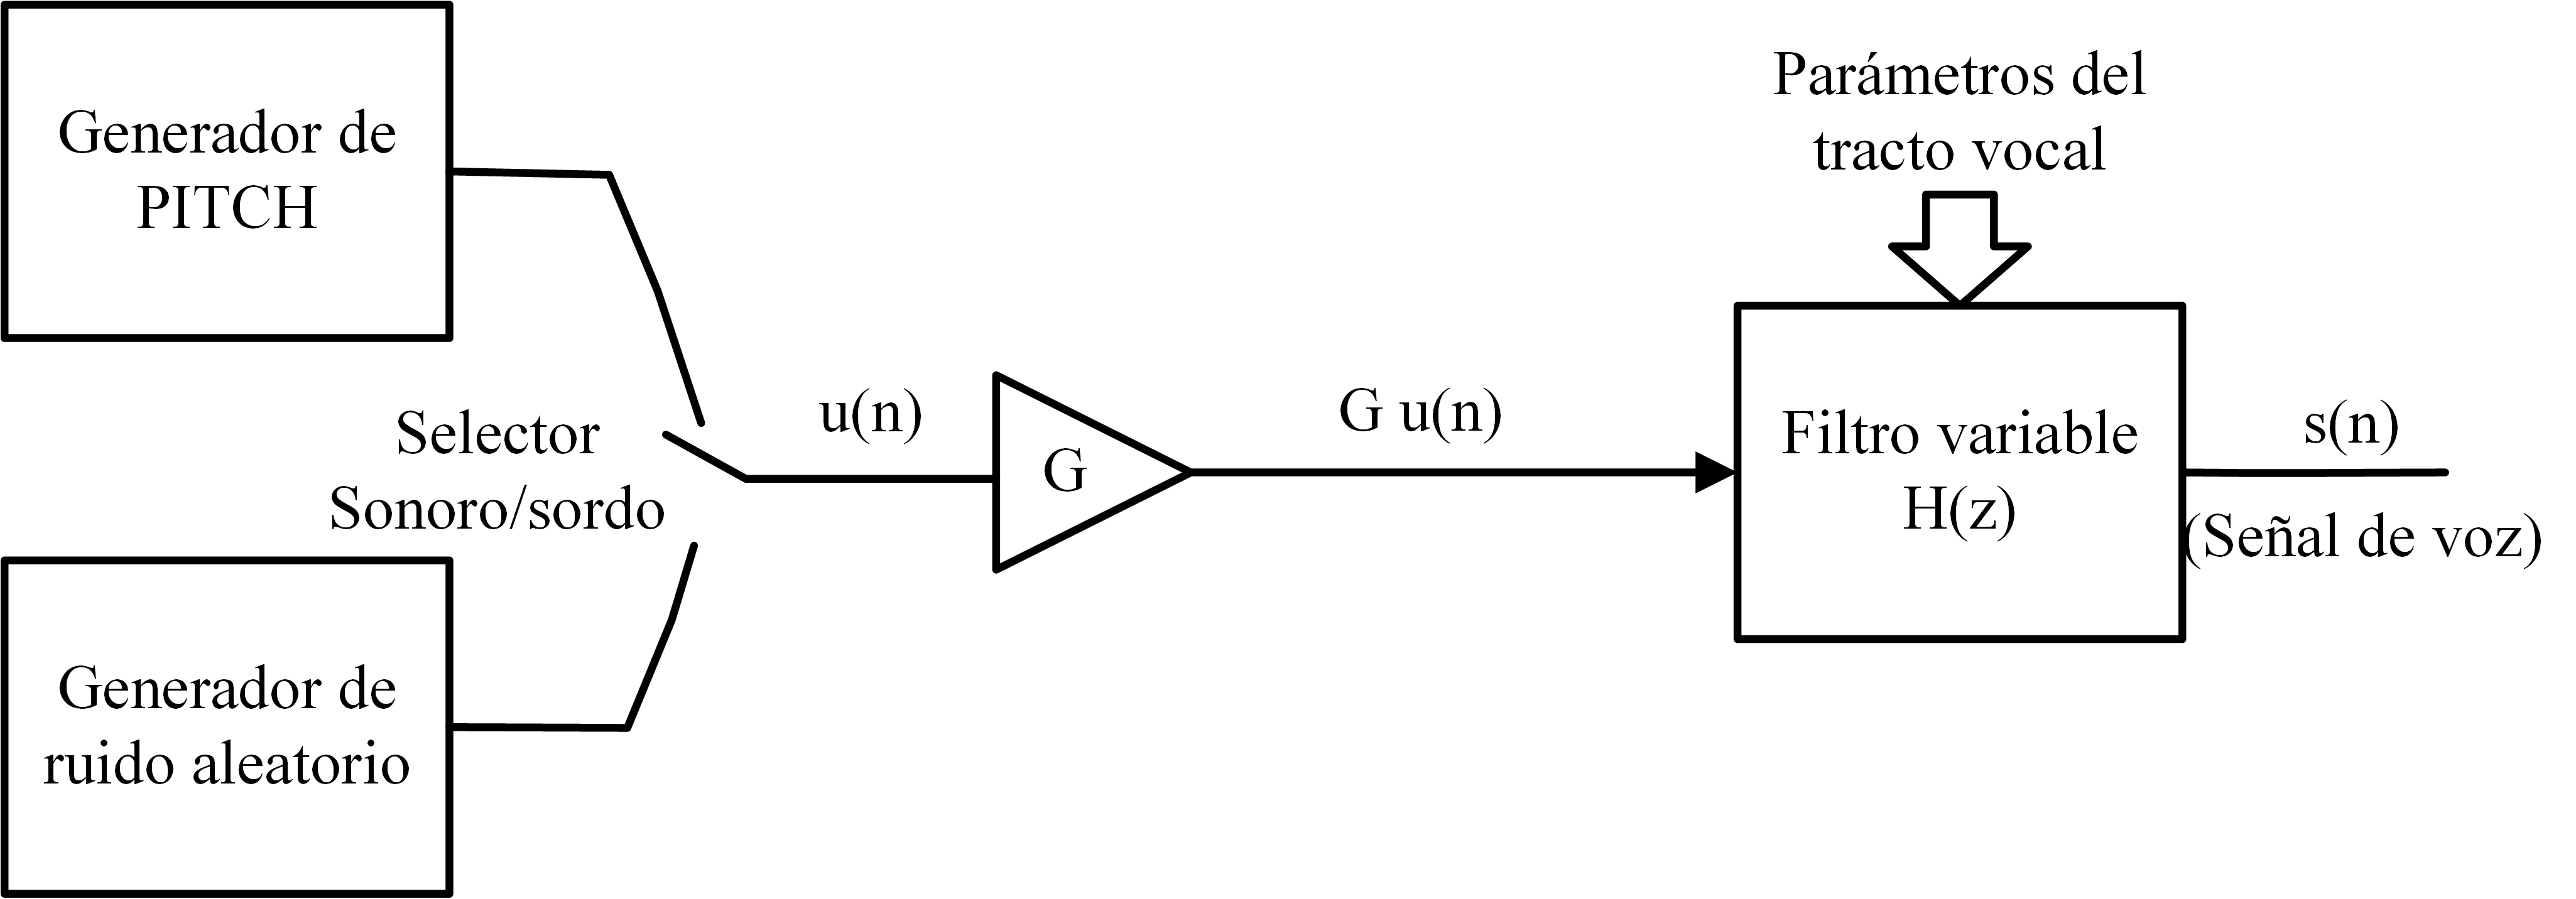
\includegraphics[width=0.8\linewidth]{figures/modeloSimplificado}
	\caption{Modelo Simplificado de la producción de la voz}
	\label{fig:modeloSimplificado}
\end{figure}

\subsection{Fonemas}

Los fonemas (sonido de la voz humana) son unidades teóricas básicas postuladas para estudiar el nivel fónico-fonológico de una lengua humana. Un fonema es cada una de las unidades segméntales postuladas para un sistema fonológico que dé cuenta de los sonidos de una lengua.

Los fonemas son la representación mental de un sonido, por ejemplo, si varias personas pronuncian la palabra tren, se notarán diferencias en la pronunciación más o menos marcadas, la t sonará más o menos enérgica, la r vibrará más o menos, estas variaciones serán notables, aunque la palabra sea pronunciada por el mismo hablante en situaciones diferentes. En la Figura \ref{fig:trenWord} se puede observar la pronunciación de la palabra Tren por tres personas diferentes, en este caso podemos observar las variaciones de amplitud de las palabras, y su duración. El sonido es la realización física de un fonema, en estos casos, podemos observar los diferentes sonidos que se generaron pero que corresponden al mismo fonema, por lo tanto, éstos son innumerables, tantos como hablantes y tantos como empleos le da cada hablante.

\begin{figure}[H]
	\centering
	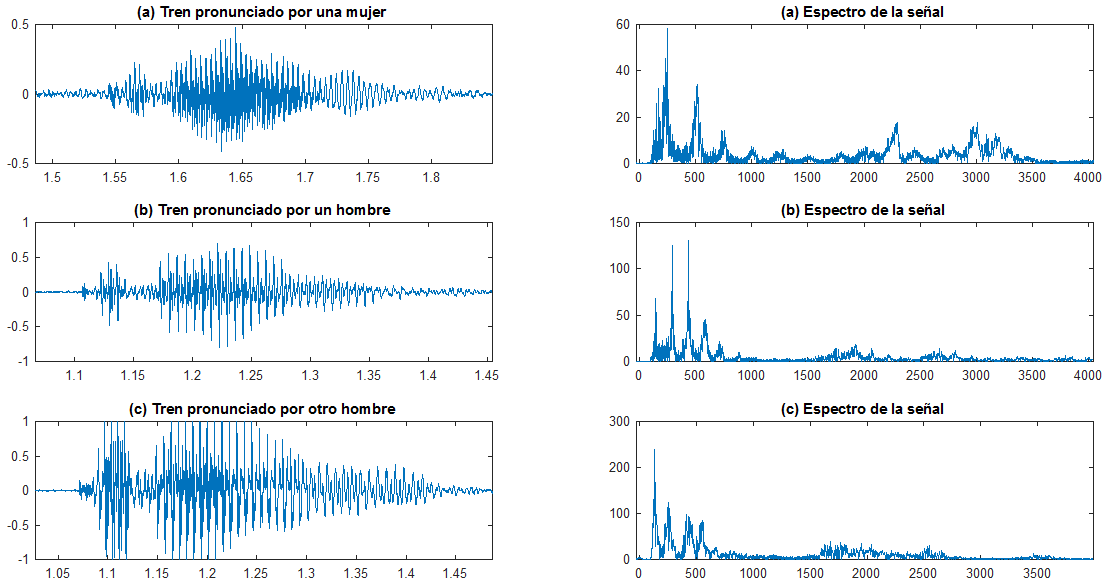
\includegraphics[width=1\linewidth]{figures/trenWord}
	\caption{Pronunciación de la palabra ''Tren''}
	\label{fig:trenWord}
\end{figure}

En la Figura \ref{fig:trenWord} podemos observar la diferencia de duración de pronunciación de palabras y la amplitud de la forma de onda que son las diferencias más visibles, por otro lado en el espectro de la señal se puede observar una gran diferencia entre el hombre y la mujer, ya que la mujer alcanza mayores frecuencias, incluso, la frecuencia fundamental está por encima de la de los hombres.

El sonido producido por las cuerdas vocales se le puede llamar un sonido “en bruto” ya que no ha sido modificado por la boca, este sonido en bruto al llegar a la boca es modificado para convertirse en sonido. Esta modificación es a lo que se le llama articulación. Articulación es la posición que adoptan los órganos de la boca en el momento de producir un sonido. Los órganos articuladores se clasifican en dos tipos:

\begin{itemize}
\item	Activos: éstos son el labio, la lengua, los dientes inferiores, velo del paladar. 
\item	Pasivos: dientes superiores, alvéolos\footnote{Los alvéolos son los hoyos donde están encajados los dientes, pero en fonética dicha palabra se refiere únicamente a las encías superiores, la zona en la que se apoya la lengua al pronunciar la n.}  superiores y paladar.
\end{itemize}

\subsubsection{Fonemas vocálicos}

Cuando articulamos los sonidos vocálicos, el aire no encuentra obstáculos en su salida desde los pulmones al exterior. Para clasificar estos fonemas, se tienen en cuenta los siguientes factores:

\begin{itemize}
\item	La localización o punto de articulación: Se refiere a la parte de la boca donde se articulan, pueden ser anteriores (/e/, /i/), medio o central (/a/) o posteriores (/o/, /u/).
\item	La abertura o modo de articulación: Se refiere a la abertura de la boca al pronunciarlos. Pueden ser de abertura máxima o abierto (/a/), de abertura media o semiabiertos (/e/, /o/) y de abertura mínima o cerrados (/i/, /u/). \cite{SantosPosada2004}
\end{itemize}

En la Figura \ref{fig:trianguloArticulatorio} se observa el triángulo articulatorio de las vocales o triángulo de Hellwag, el cual nos describe la localización y la abertura para cada fonema vocálico.

\begin{figure}[H]
	\centering
	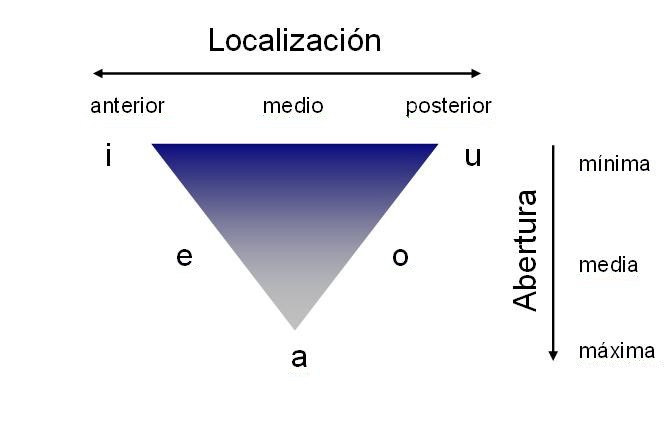
\includegraphics[width=0.8\linewidth]{figures/trianguloArticulatorio}
	\caption{Triángulo articulatorio de las vocales}
	\label{fig:trianguloArticulatorio}
\end{figure}

\subsubsection{Fonemas consonánticos}

En la articulación de los sonidos consonánticos siempre hay un obstáculo que impide salir el aire desde los pulmones al exterior. Según las circunstancias que rodean esta salida de aire, existen ciertos factores a tomar en cuenta a la hora de clasificarlos.

\begin{itemize}
\item	Zona o punto de articulación: Es el lugar donde toman contacto los órganos que intervienen en la producción del sonido.
\begin{itemize}
\item	Bilabial: Los dos labios.
\item	Labiodental: Labio inferior y dientes superiores.
\item	Interdental: Lengua entre los dientes.
\item	Dental: Lengua detrás de los dientes superiores.
\item	Alveolar: Lengua sobre la raíz de los dientes superiores.
\item	Palatal: Lengua y paladar.
\item	Velar: Lengua y velo del paladar.
\end{itemize}
\item	Modo de articulación: Es la postura que adoptan los órganos que producen los sonidos.
\begin{itemize}
\item	Oclusivo: Cierre total y momentáneo del paso del aire.
\item	Fricativo: Estrechamiento por donde pasa el aire rozando.
\item	Africado: Se produce una oclusión y después una fricación.
\item	Lateral: El aire pasa rozando los lados de la cavidad bucal.
\item	Vibrante: El aire hace vibrar la punta de la lengua al pasar.
\end{itemize}
\item	Actividad de las cuerdas vocales: Cuando producimos sonidos, las cuerdas vocales pueden vibrar o no vibrar.
\begin{itemize}
\item	Sordo: No vibran las cuerdas vocales.
\item	Sonoro: Vibran las cuerdas vocales.
\end{itemize}
\item	Actividad de la cavidad nasal: Si al producir sonidos, parte del aire pasa por la cavidad nasal, los sonidos se llaman nasales.
\begin{itemize}
\item	Nasal: Parte del aire pasa por la cavidad nasal.
\item	Oral: Todo el aire pasa por la boca.
\end{itemize}
\end{itemize}

En la Figura \ref{fig:fonemasConsonantes} se presentan los fonemas consonantes de acuerdo a los factores y rasgos mencionados anteriormente.

\begin{figure}[H]
	\centering
	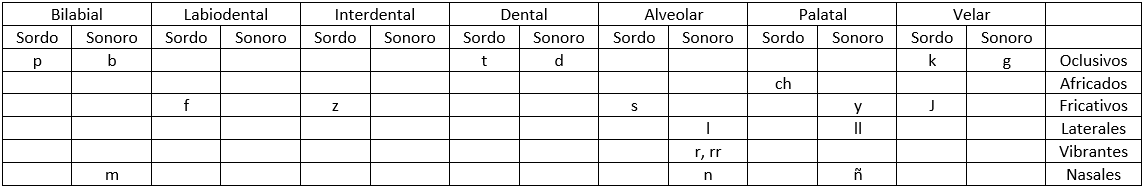
\includegraphics[width=1\linewidth]{figures/fonemasConsonantes}
	\caption{Cuadro de los fonemas consonantes}
	\label{fig:fonemasConsonantes}
\end{figure}

% Please add the following required packages to your document preamble:
% \usepackage{booktabs}
%\begin{table}[H]
%\centering
%\caption{My caption}
%\label{tbl:fonemas}
%\begin{tabular}{|p{0.8cm} |p{0.8cm} |p{0.8cm} |p{0.8cm} |p{0.8cm} |p{0.8cm} |p{0.8cm} |p{0.8cm} |p{0.8cm} |p{0.8cm} |p{0.8cm} |p{0.8cm} |p{0.8cm} |p{0.8cm} |p{0.8cm}|  }
%\toprule
%\multicolumn{2}{|c|}{Bilabial} & \multicolumn{2}{c|}{Labiodental} & \multicolumn{2}{c|}{Interdental} & \multicolumn{2}{c|}{Dental} & \multicolumn{2}{c|}{Alveolar} & \multicolumn{2}{c|}{Palatal} & \multicolumn{2}{c|}{Velar} &            \\ \midrule
%Sordo         & Sonoro         & Sordo          & Sonoro          & Sordo          & Sonoro          & Sordo        & Sonoro       & Sordo         & Sonoro        & Sordo        & Sonoro        & Sordo       & Sonoro       &            \\ \midrule
%p             & b              &                &                 &                &                 & t            & d            &               &               &              &               & k           & g            & Oclusivos  \\ \midrule
%              &                &                &                 &                &                 &              &              &               &               & ch           &               &             &              & Africados  \\ \midrule
%              &                & f              &                 & z              &                 &              &              & s             &               &              & y             & j           &              & Fricativos \\ \midrule
%              &                &                &                 &                &                 &              &              &               & l             &              & ll            &             &              & Laterales  \\ \midrule
%              &                &                &                 &                &                 &              &              &               & r, rr         &              &               &             &              & Vibrantes  \\ \midrule
%              & m              &                &                 &                &                 &              &              &               & n             &              & ñ             &             &              & Nasales    \\ \bottomrule
%\end{tabular}
%\end{table}

\subsection{Digitalización de la señal de voz}

La parte inicial de todo subsistema de preproceso de la señal de voz está constituida por:
\begin{itemize}
\item	Un micrófono, que convierte la onda sonora de presión en una señal eléctrica.
\item	Un amplificador, que amplifica hasta niveles manejables la débil señal que proporciona el micrófono.
\end{itemize}


\subsubsection{Muestreo y cuantificación}

A partir de la señal eléctrica que produce el amplificador se termina por digitalizar la señal de voz por un convertidor analógico/digital, éste, básicamente debe realizar dos tareas:

\begin{itemize}
\item	Muestrear la señal analógica; es decir, medir la amplitud de dicha señal cada cierto intervalo de tiempo.
\item	Cuantificar la señal muestreada; es decir, codificar numéricamente el resultado de cada una de las medidas.
\end{itemize}
De esta manera, una función continua del tiempo quedará representada por una serie discreta de valores numéricos.

\subsubsection*{Muestreo}

Una señal muestreada a intervalos de tiempo $T, s_M (t)$, puede definirse como el producto de la señal continua $s(t)$ y una función de Dirac (Figura \ref{fig:muestreoDelta}):

\begin{equation}\label{eq:muestreo}
	s_M(t)=s(t) \cdot \sum_{k=-\infty}^{\infty}\delta(t-KT)=\sum_{k=-\infty}^{\infty}s(kT)\delta(t-KT)
%	y = f \left[ \left( \sum_{i=1}^{N}\omega_i*x\left(n-i\right)\right)-b	\right]
\end{equation}

Donde:
\\$s_M->$ señal muestreada.
\\$s->$ señal a muestrear.		

\begin{figure}[H]
	\centering
	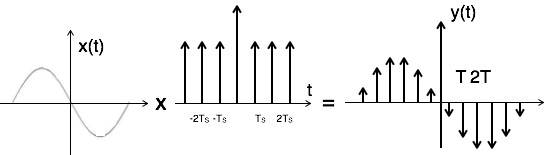
\includegraphics[width=0.6\linewidth]{figures/muestreoDelta}
	\caption{Muestreo de una señal}
	\label{fig:muestreoDelta}
\end{figure}

De donde es inmediato demostrar que la expresión del espectro $S_M (j\omega)$ de la señal muestreada en función de la señal sin muestrear $S(j\omega)$, adopta la forma:

\begin{equation}\label{eq:muestreoEspectro}
	S_M(j\omega)=\frac{1}{T}\sum_{k=-\infty}^{\infty}S[j(\omega+k\omega_0)] ;	 \omega_0=\frac{2\pi}{T}
%	y = f \left[ \left( \sum_{i=1}^{N}\omega_i*x\left(n-i\right)\right)-b	\right]
\end{equation}	

Expresión que representa la superposición del espectro de s(t) con las sucesivas versiones del mismo desplazadas en el eje de la frecuencia con periodicidad $\frac{1}{T}$.

De la Figura \ref{fig:aliasing} se observa que, si el ancho de banda de la señal a muestrear es excesivo con relación a la frecuencia de muestreo, se producirá un solapamiento irreversible de los espectros sucesivos, haciendo imposible la reconstrucción de la señal original. Este solapamiento (aliasing) ocurre siempre que la máxima frecuencia (Fb) del espectro de la señal a muestrear sea superior a la mitad de la frecuencia de muestreo (Fm) (frecuencia de Nyquist).

\begin{figure}[H]
	\centering
	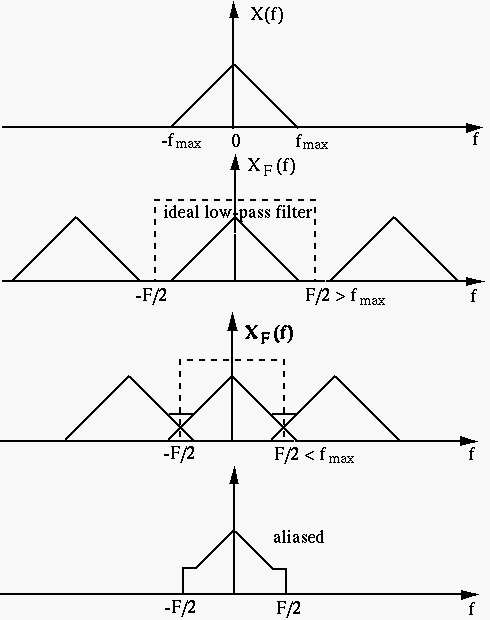
\includegraphics[scale = 0.6]{figures/aliasing}
	\caption{Efecto de solapamiento ''aliasing''}
	\label{fig:aliasing}
\end{figure}

Antes de muestrear una señal será pues necesario limitar la frecuencia máxima de ésta a la mitad de la de muestreo, lo que se puede conseguir mediante un filtro analógico de paso bajo previo al convertidor A/D, cuya frecuencia de corte sea la de Nyquist como máximo. La anchura de banda de la señal resultante deberá preservar la información relevante necesaria para una adecuada descripción de los objetos acústicos a tratar. \cite{Casacuberta1987}

\subsubsection*{Cuantificación}

El cuantificador es un sistema no lineal cuyo propósito es transformar la muestra de entrada $x[n]$ en un valor de un conjunto finito de valores preestablecidos. Representada como

\begin{equation}\label{eq:cuantificador}
	\hat{x}[n]=Q(x[n])
%	y = f \left[ \left( \sum_{i=1}^{N}\omega_i*x\left(n-i\right)\right)-b	\right]
\end{equation}	

Donde $\hat{x}[n]$ es la muestra cuantificada.

Los cuantificadores se pueden definir con niveles de cuantificación uniformes o no uniformes. La Figura \ref{fig:cuantificadorTipico} muestra la característica de transferencia de un cuantificador uniforme en el que los valores de las muestras se redondean hasta el nivel de cuantificación más próximo.

\begin{figure}[H]
	\centering
	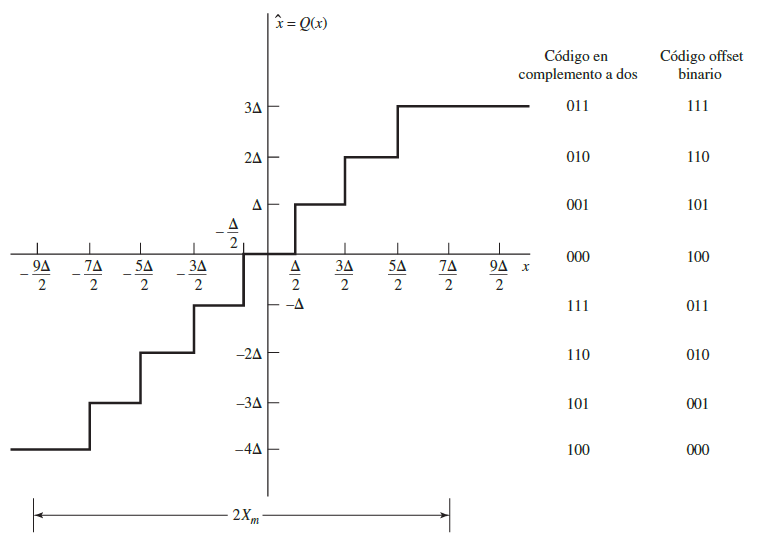
\includegraphics[scale = 0.6]{figures/cuantificadorTipico}
	\caption{Cuantificador típico para conversión A/D. (Tomado de \cite{Oppenheim2011})}
	\label{fig:cuantificadorTipico}
\end{figure}

\subsection{Métodos en el dominio del tiempo para el procesamiento del habla}

El objetivo en el procesamiento del habla es obtener la representación más útil de la información que lleva la señal de voz. La precisión requerida de esta representación está dada por información particular de la señal de voz que va a ser preservada o, en ciertos casos, resaltarla. Por ejemplo, el propósito del procesamiento digital puede ser para facilitar la identificación de la forma de onda correspondiente a voz o no. En una aplicación similar pero más complejo, queremos clasificar la señal de voz en 3 tipos, voz sonora, voz no sonora y silencio o ruido de fondo.

En esta sección se presentan técnicas de procesamiento en el dominio del tiempo.

\subsubsection{Procesamiento del habla dependiente del tiempo}

En la Figura \ref{fig:vozTipica} se muestra la representación típica de la señal de voz en la cual se aprecia que las propiedades de la voz cambian en el tiempo. Por ejemplo, la excitación cambia entre la señal sonora y la no sonora, hay variaciones significantes en la amplitud pico de la señal y hay una variación considerable de la frecuencia fundamental en las regiones de señal sonora.

\begin{figure}[H]
	\centering
	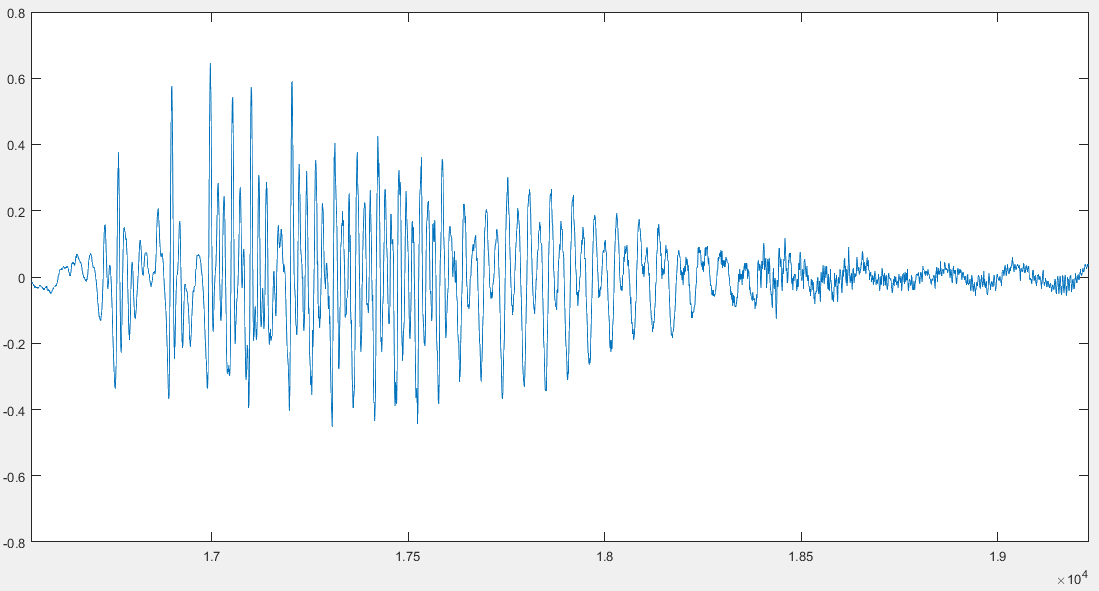
\includegraphics[width=1\linewidth]{figures/vozTipica}
	\caption{Señal de voz}
	\label{fig:vozTipica}
\end{figure}

Estas variaciones son evidentes en una gráfica de la forma de onda en el dominio del tiempo, por lo cual, las técnicas de procesamiento deben ser capaces de ofrecernos representaciones útiles de las características de la señal como la intensidad, modo de excitación, tono, y posiblemente parámetros del tracto vocal como frecuencias formantes.

La suposición en muchos esquemas de procesamiento del habla es que las propiedades de la señal cambian relativamente lento con el tiempo. Esta suposición deja una variedad de métodos de procesamiento en tiempo corto en donde segmentos cortos de la señal de voz son aislados y procesados como si fueran segmentos cortos de un sonido prolongado con propiedades fijas. El resultado del procesamiento de cada segmento puede ser tanto un número, o un conjunto de números. Por lo tanto, tal procesamiento produce una nueva secuencia dependiente del tiempo que puede servir como una representación de la señal de voz.

La mayoría de las técnicas de procesamiento en corto tiempo, así como la representación de Fourier en tiempo corto, pueden ser representadas matemáticamente con la ecuación \ref{eq:windowing}

\begin{equation}\label{eq:windowing}
	Q_n=\sum_{m=-\infty}^{\infty}{T[x(m)]w(n-m)}
%	y = f \left[ \left( \sum_{i=1}^{N}\omega_i*x\left(n-i\right)\right)-b	\right]
\end{equation}

La señal de voz es sujeta a una transformación, T[ ], que puede ser linear o no linear. La secuencia resultante es multiplicada por una ventana ubicada en un momento correspondiente al índice de muestra m. 

Una de las características de la seña de voz es la energía, ésta en una señal de tiempo se define como:

\begin{equation}\label{eq:windowing}
	E=\sum_{m=-\infty}^{\infty}{x^2(m)}
\end{equation}

Donde:
\\$E->$ energía de la señal.
\\$x->$ señal de tiempo.

Tal cantidad tiene poco significado o utilidad para el habla ya que da poca información acerca de las propiedades dependientes del tiempo de la señal de voz. La definición de la energía en poco tiempo es:

\begin{equation}\label{eq:windowing}
	E_n=\sum_{m=n-N+1}^{n}{x^2(m)}
\end{equation}

\subsubsection{Energía de corta duración y media de magnitud}

Se ha observado que la amplitud de la señal de voz varía con el tiempo. En particular, la amplitud de los segmentos de la señal no sonora es generalmente menor que la amplitud de los segmentos de señal sonora. La energía de corta duración de la señal de voz ofrece una representación conveniente que refleja estas variaciones de amplitud. En general, se puede definir la energía de corta duración como

\begin{equation}\label{eq:windowing}
	E_n=\sum_{m=-\infty}^{\infty}{[x(m)w(n-m)]^2}
\end{equation}

Donde:
\\$E_n->$ energía de corta duración.
\\$x->$ señal de voz.
\\$w->$ ventana aplicada.

$E_n$ proporciona una base para distinguir los segmentos de voz sonora delos segmentos de voz no sonora. Como se muestran en la Figura \ref{fig:energiaRectangular} y Figura \ref{fig:energiaHamming}, los valores de$ E_n$ para los segmentos de voz no sonora son menores que para los de la voz sonora. La función de energía también se puede usar para localizar aproximadamente el tiempo en el cual la voz sonora se convierte en voz no sonora, y viceversa, y, para una señal de muy alta calidad (alta relación señal a ruido), la energía puede ser usada para distinguir la voz del silencio.

\begin{figure}[H]
	\centering
	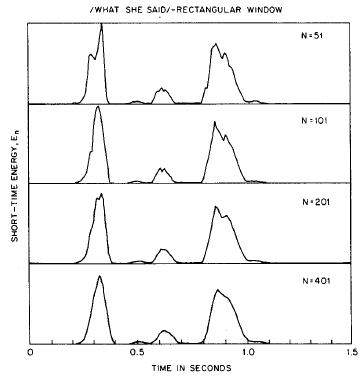
\includegraphics[width=0.5\linewidth]{figures/energiaRectangular}
	\caption{Energía en tiempo corto con ventana rectangular de varios tamaños}
	\label{fig:energiaRectangular}
\end{figure}

\begin{figure}[H]
	\centering
	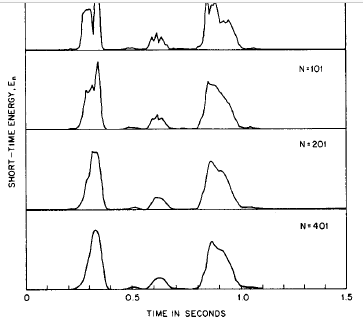
\includegraphics[width=0.5\linewidth]{figures/energiaHamming}
	\caption{Función de energía en periodo corto con ventana de Hamming en varios tamaños}
	\label{fig:energiaHamming}
\end{figure}

El promedio de la magnitud también es usado en el procesamiento de voz y aplicado a las señales de voz, la función de magnitud está dada por:

\begin{equation}\label{eq:promedio}
	M_n=\sum_{m=-\infty}^{\infty}{|x(m)|w(n-m)}
\end{equation}

Donde:
\\$M_n->$ promedio de magnitud.

Donde la suma ponderada de los valores absolutos de la señal es calculada en vez de la suma de cuadrados. La Figura \ref{fig:energiaFiltro} muestra cómo puede ser implementado como un filtro lineal sobre el absoluto de la señal. Este método logra simplificar aritméticamente la operación eliminando la operación de elevación al cuadrado.

\begin{figure}[H]
	\centering
	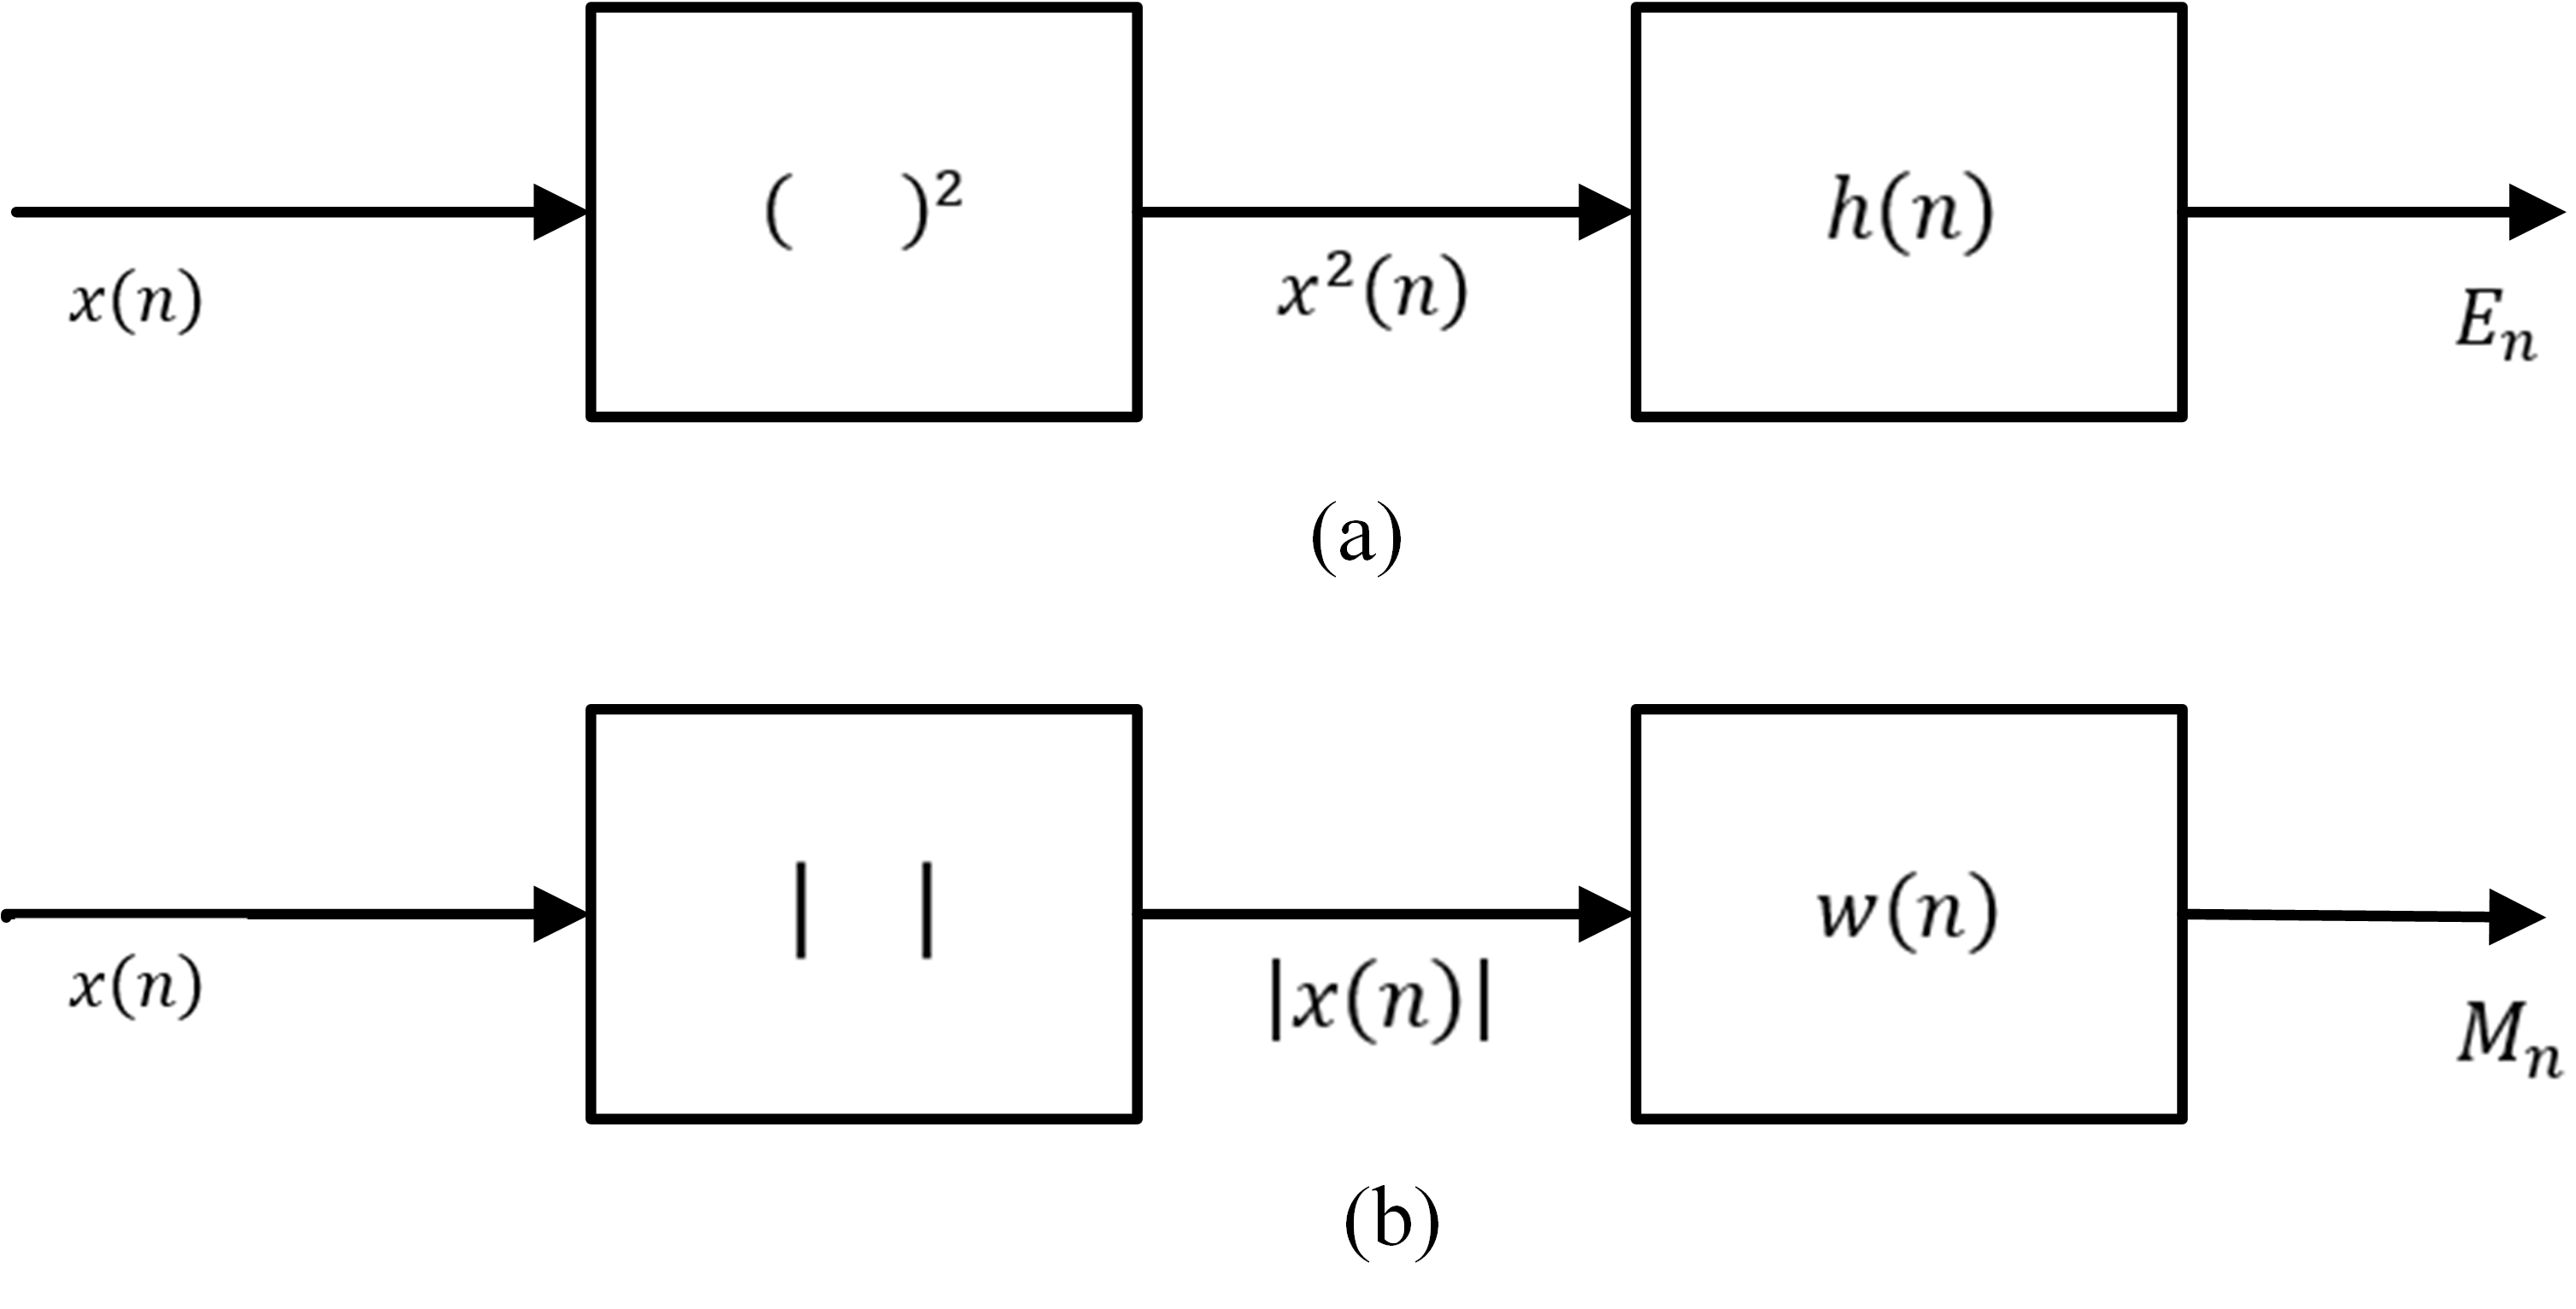
\includegraphics[width=0.5\linewidth]{figures/energiaFiltro}
	\caption{(a) Implementación del cálculo de la energía mediante un filtro. (b) implementación del cálculo de la magnitud promedio mediante un filtro}
	\label{fig:energiaFiltro}
\end{figure}

En la Figura \ref{fig:promedioRectangular} y Figura \ref{fig:promedioHamming} muestran las gráficas del promedio de la magnitud, en comparación con los resultados por el método de la energía se pueden observar diferencias muy notables en las regiones no sonoras. Para el promedio de la magnitud, el rango dinámico es aproximadamente la raíz cuadrada que el rango dinámico para el cálculo por energía. Por lo tanto, las diferencias de nivel entre las regiones sonoras y no sonoras no son tan notables como para el cálculo de energía en tiempo corto.

\begin{figure}[H]
	\centering
	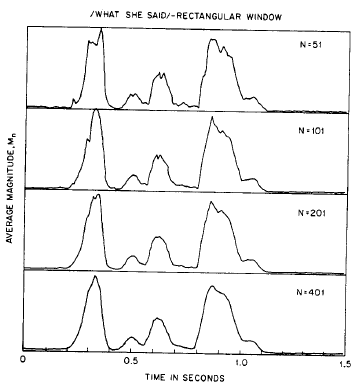
\includegraphics[width=0.5\linewidth]{figures/promedioRectangular}
	\caption{Promedio de magnitud con ventana rectangular}
	\label{fig:promedioRectangular}
\end{figure}

\begin{figure}[H]
	\centering
	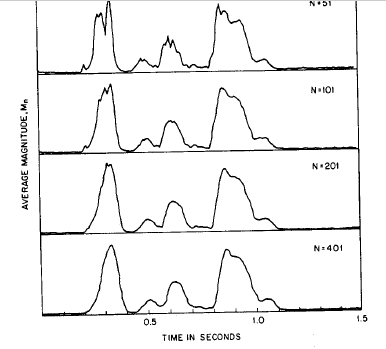
\includegraphics[width=0.5\linewidth]{figures/promedioHamming}
	\caption{Promedio de magnitud con ventana Hamming}
	\label{fig:promedioHamming}
\end{figure}

\subsubsection{Cruces por cero}

En señales discretas en tiempo, un cruce por cero se dice que ocurre si muestras sucesivas tienen diferente signo algebraico. La velocidad a la cual los cruces por cero ocurren es una simple medida del contenido de frecuencia de una señal. Esto es particularmente cierto en señales de banda estrecha. Por ejemplo, una señal sinusoidal de frecuencia $f_0$ muestreada a una tasa $f_s$, tiene $\frac{f_s}{f_0}$  muestras por periodo de la señal sinusoidal. Cada periodo tiene dos cruces por cero así que la tasa promedio de cruces por cero es:

\begin{equation}\label{eq:promedio}
	Z=2\frac{f_0}{f_s}
\end{equation}
Donde:
\\$Z->$ tasa promedio de cruces por cero de una señal sinusoidal.

Así, el promedio de la tasa de cruces por cero da una vía razonable para estimar la frecuencia de la señal sinusoidal.

Señales de voz son señales de banda ancha y la interpretación del promedio de la tasa de cruces es por lo tanto mucho menos precisa. Como sea, estimaciones aproximadas de las propiedades espectrales se pueden obtener usando una representación basada en el promedio de la tasa de cruces por cero en tiempo corto. Una definición apropiada del promedio de cruces por cero está dada por:


\begin{equation}\label{eq:zeroCross}
	Z_n=\sum_{m=-\infty}^{\infty}{|sgn[x(m)]-sgn[x(m-1)]|w(n-m)}
\end{equation}

Donde

\begin{equation}\label{eq:promedio}
	sgn[x(n)]= 
\begin{cases}
    1,	& x(n)\geq0\\
    -1,              & x(n)<0
\end{cases}
\end{equation}

y

\begin{equation}\label{eq:promedio}
	w(n)= 
\begin{cases}
    \frac{1}{2N},	& 0\leq n\leq N-1\\
    -1,              & \text{otro caso}
\end{cases}
\end{equation}

Las operaciones de (\ref{eq:zeroCross}) están representadas en un diagrama de bloques de la Figura \ref{fig:crucesCero}.

\begin{figure}[H]
	\centering
	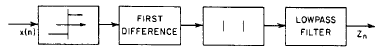
\includegraphics[width=0.6\linewidth]{figures/crucesCero}
	\caption{Diagrama a bloques del cálculo de cruces por cero}
	\label{fig:crucesCero}
\end{figure}

La representación muestra que el promedio de la tasa de cruces por cero en tiempo corto tiene las mismas propiedades generales que el promedio de energía y magnitud en tiempo corto.

El modelo de producción de la voz sugiere que la energía de la señal sonora está concentrada por debajo de los 3kHz, mientras que, para señales no sonoras, la mayor parte de la energía se encuentra en altas frecuencias. Desde altas frecuencias implica altas tasas de cruce por cero, y bajas frecuencias implican bajas tasas de cruce por cero, hay una fuerte correlación entre tasa de cruces por cero y distribución de energía con frecuencia. Una generalización es que, si la tasa de cruces por cero es alta, la señal de voz es no sonora, mientras que, si la tasa de cruces por cero es baja, la señal de voz es sonora. Esto, sin embargo, esta declaración es muy imprecisa porque no se tiene una forma de decir qué es alto y qué es bajo.

En la Figura \ref{fig:gaussianHisto} se muestra un histograma del promedio de la tasa de cruces por cero para señal sonora y no sonora. La media del promedio de la tasa de cruces por cero en tiempo corto es de 49 cada 10 ms para señal no sonora y 14 cada 10 ms para sonora. Claramente las dos distribuciones se traslapan por lo que una decisión inequívoca de sonora y no sonora no es posible basado únicamente en el promedio de cruces por cero en tiempo corto.

\begin{figure}[H]
	\centering
	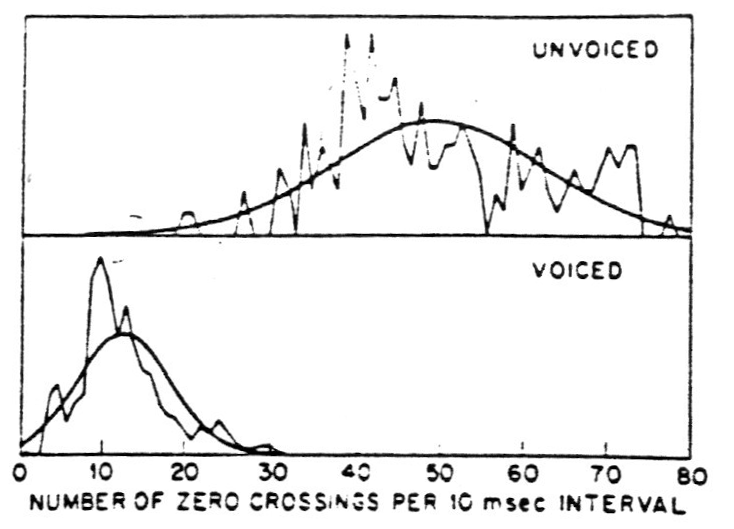
\includegraphics[width=0.6\linewidth]{figures/gaussianHisto}
	\caption{Cruces por cero en un intervalo de 10 ms}
	\label{fig:gaussianHisto}
\end{figure}

La aplicación del procesamiento de voz a cualquier tarea requiere el entendimiento previo de las características de la voz y el tratamiento que se le debe dar de acuerdo al fin que se desee. En particular para el reconocimiento del habla, el esquema de procesamiento que se sigue es similar al presentado en la Figura \ref{fig:esquemaReconocimiento}.

\begin{figure}[H]
	\centering
	
\includegraphics[width=0.8\linewidth]{figures/esquemaReconocimiento}
	\caption{Esquema general del reconocimiento de voz}
	\label{fig:esquemaReconocimiento}
\end{figure}

Es necesario entender las bases para llevar a cabo el reconocimiento de voz, para esto, se describen los bloques presentados en la Figura \ref{fig:esquemaReconocimiento}, lo cual nos llevará a decidir las mejores técnicas a emplear para llevar a cabo este proceso. \cite{SalcedoCherubini2006}

\subsection{Pre-procesamiento}

La etapa de pre-procesamiento corresponde a los pasos previos a la parametrización de la señal de voz, estos pasos son necesarios para resaltar las características más importantes y posteriormente analizarlas con las técnicas de parametrización. La Figura \ref{fig:preProcesamiento} muestra el diagrama a bloques del pre-procesamiento propuesto.

\begin{figure}[H]
	\centering
	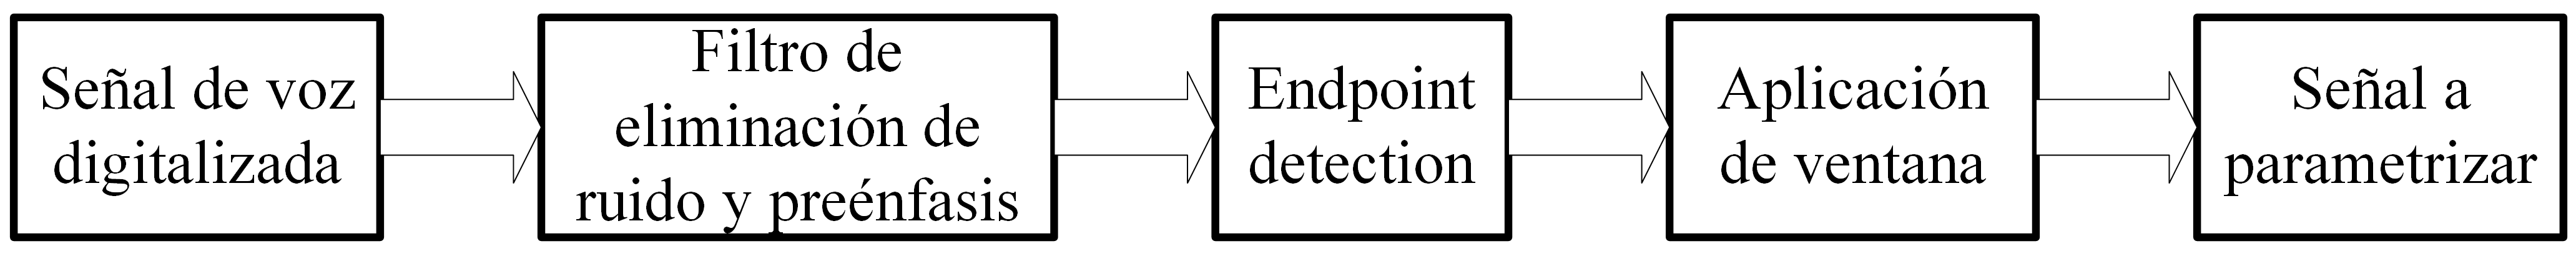
\includegraphics[width=0.9\linewidth]{figures/preProcesamiento}
	\caption{Diagrama a bloques del pre-procesamiento}
	\label{fig:preProcesamiento}
\end{figure}

A continuación, se detalla cada bloque presentado en la Figura \ref{fig:preProcesamiento}. Cabe mencionar que la señal de voz digitalizada, es el resultado de los procesos de adquisición de la voz a través del micrófono y la conversión analógica-digital.

\subsubsection{Filtro preénfasis}

La etapa de preénfasis se realiza para hacer el procesamiento de la señal menos susceptible a truncamientos, aplanarla espectralmente y compensar la caída de 6dB que experimenta la señal al pasar a través del tracto vocal. Generalmente se usa un filtro digital de primer orden cuya función de transferencia es la que se muestra en la ecuación (\ref{eq:preenfasis}). \cite{SalcedoCherubini2006}

\begin{equation}\label{eq:preenfasis}
	H(z)=1-az^{-1}
\end{equation}

Donde a toma valores entre [0.9, 0.95], valor cercano a la unidad a fin de que la estructura de los formantes mayores sea acentuada. La salida de la etapa de preénfasis está dada por la ecuación (\ref{eq:salidaPreenfasis}).

\begin{equation}\label{eq:salidaPreenfasis}
	\tilde{s}(n)=s(n)-a\cdot s(n-1)
\end{equation}

Donde:
\\$\tilde{s}->$ señal filtrada.
\\$s->$ señal de voz.

\subsubsection{Endpoint detection}

Un problema importante en el procesamiento del habla es el detectar la presencia del habla en un ambiente ruidoso. Este problema es comúnmente conocido como \textit{endpoint location problem}. La detección precisa del inicio y fin de una palabra significa que el procesamiento posterior se puede mantener a un mínimo logrando optimizar recursos.

Una de las principales causas de los errores en sistemas de reconocimiento del habla en palabras aisladas es la detección inexacta de los límites inicial y final en los patrones de prueba y de referencia. Es esencial en los sistemas de reconocimiento automático del habla que los segmentos de habla puedan separarse de forma fiable de los segmentos de no habla.

Requerimientos del algoritmo:

\begin{itemize}
\item	Fiabilidad y robustez: el endpointer sin supervisión automática debe ser fiable, es decir, lo suficientemente robusta como para evitar errores de clasificación en las condiciones de trabajo difíciles, tales como la variación de la relación señal a ruido, intensidad variable, etc.
\item	Precisión: Mínima pérdida de segmentos como los siguientes no es admisible
\begin{itemize}
\item	Inicio o término de palabras con fonemas de baja energía.
\item	Oclusiva sorda.
\item	Una nasal.
\item	Una respiración corta, golpe, o ligero ruido.
\end{itemize}
\item	Adaptabilidad: el algoritmo debe ser adaptivo para ser capaz de hacer frente a los cambios del entorno, especialmente el ruido de fondo variable.
\item	Simplicidad: la simplicidad es otra característica deseada de especial importancia cuando el algoritmo está pensado como parte del reconocedor. Por ejemplo, los algoritmos que manejan condiciones difíciles tales como el habla de telefonía suelen ser muy compleja.
\item	Procesamiento en tiempo real: también se desea el procesamiento en tiempo real y sólo es posible si el algoritmo no es complejo.
\item	No conocimiento a priori de ruido: se requiere en un algoritmo ideal que debe ser capaz de hacer frente a la variación de la relación señal a ruido.
\end{itemize}

El algoritmo propuesto en \cite{Rabiner1975} usa dos medidas de la señal, la energía y la tasa de cruces por cero.

Tres umbrales se calculan:

\begin{itemize}
\item	ITU – Upper energy threshold
\item	ITL – Lower energy threshold
\item	IZCT – Zero crossings rate threshold
\end{itemize}

\subsubsection{Aplicación de ventana}

En la etapa siguiente, la señal filtrada y sin silencios, obteniendo así la información útil de la voz, se hace necesario dividir la señal en tramas de N muestras, donde N es un valor que se escoge tomando en cuenta que la señal de voz es estacionaria a segmentos; condición necesaria para realizar el análisis de Fourier en tiempo corto. El intervalo de tiempo en el que la señal de voz se considera estacionaria depende de la velocidad de cambios del tracto vocal y las cuerdas vocales, comúnmente se establece un valor entre 20 y 40 ms. \cite{SalcedoCherubini2006}

En la Figura \ref{fig:segmentacion} se muestra un ejemplo de segmentación utilizado comúnmente en las aplicaciones de procesamiento de voz. Por lo general se utilizan tramas de 256 muestras por ser un valor que establece un equilibrio entre la resolución en tiempo y frecuencia para una señal de voz.

\begin{figure}[H]
	\centering
	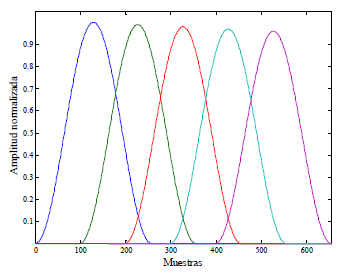
\includegraphics[width=0.6\linewidth]{figures/segmentacion}
	\caption{Segmentación de la señal de voz en tramas solapadas entre ellas.}
	\label{fig:segmentacion}
\end{figure}

Para esta fase del pre-procesamiento es importante escoger la ventana más adecuada que vamos a aplicar a nuestras tramas, para esta decisión es importante tener en cuenta el efecto de ésta sobre la resolución espectral de la señal, la cual depende del lóbulo central y la atenuación de los lóbulos laterales. Lo ideal es que el lóbulo central sea muy estrecho y los lóbulos laterales sean lo más pequeño posible.

En la Figura \ref{fig:windows} se muestran cuatro ventanas con su respectivo espectro, en la cual es fácil observar cómo es la relación del lóbulo central con sus lóbulos laterales, así como también la etnuación que tienen éstos últimos, podemos observar que la ventana de Blackman es la que presenta mayor atenuación en los lóbulos laterales con el precio de que el lóbulo central  es más ancho que las demás ventanas.

\begin{figure}[H]
	\centering
	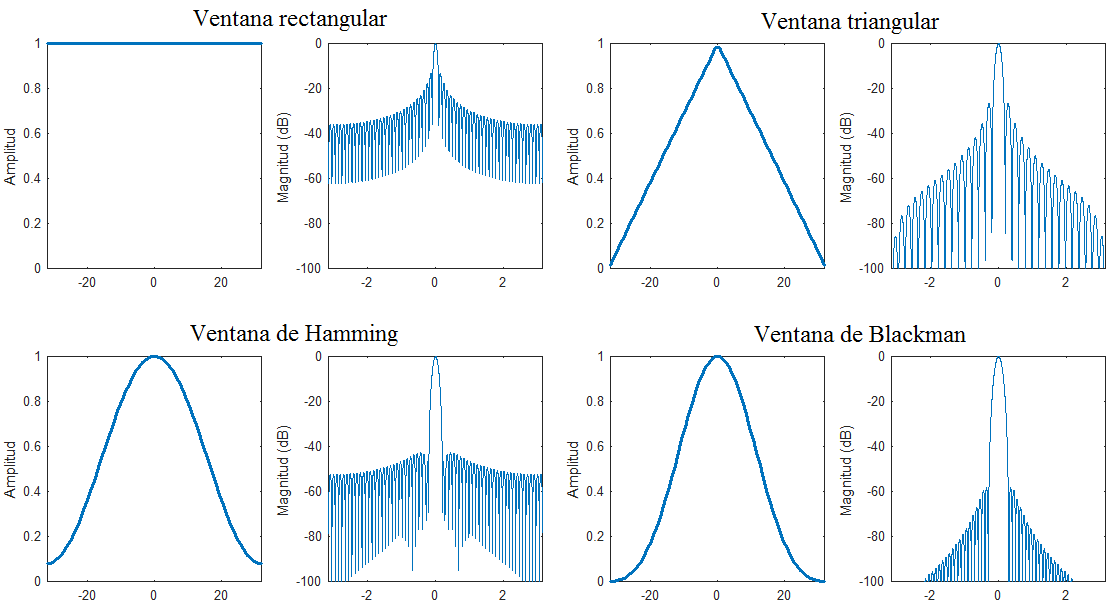
\includegraphics[width=1\linewidth]{figures/windows}
	\caption{Ventanas en el dominio del tiempo y la frecuencia.}
	\label{fig:windows}
\end{figure}

Las ventanas, tanto rectangulares y no rectangulares tienen sus ventajas y desventajas, pero dado los criterios mencionados, en el campo del procesamiento de voz la ventana de Hamming es muy utilizada, pues cumple con el requerimiento de que los lóbulos laterales sean pequeños, a pesar de que su lóbulo central es más ancho que para la ventana rectangular. La ventana de Hamming se define de acuerdo a la ecuación (\ref{eq:hammingWindow})

\begin{equation}\label{eq:hammingWindow}
	W(nT)=0.54-0.46\cdot cos(2\cdot \frac{n}{N})
\end{equation}

Donde $0<n<N$

Un aspecto importante a analizar es el solapamiento de las ventanas entre tramas consecutivas, para la Figura \ref{fig:segmentacion} es de 156 muestras y esto se lleva a cabo por dos propósitos: el primero consiste en que las mismas guarden relación entre sí para que el análisis de cada trama no sea aislado y el segundo consiste en compensar el hecho de que para la ventana de Hamming, la mayor concentración de energía se encuentra en el centro de la trama n y para compensar la caída que tiene la ventana en los bordes de la trama, se utiliza la ventana aplicada en la trama n+1. \cite{SalcedoCherubini2006}

\subsection{Parametrización}

Para cualquier sistema de reconocimiento de voz es importante hacer la selección de la mejor representación paramétrica de la señal de voz, el objetivo principal de esta representación es comprimir los datos correspondientes a la señal eliminando información no pertinente al análisis fonético de la información y extraer las características de la señal que contribuyen a la detección de las diferencias fonéticas que no son apreciables mediante un análisis en tiempo o frecuencia, para esto se hace un análisis más exhaustivo como el Cepstrum. \cite{SalcedoCherubini2006}

\subsubsection{Cepstrum}

El Cepstrum es comúnmente utilizado para la representación paramétrica de señales de voz, desde un punto de vista matemático, se puede decir que se trata de un operador que transforma una convolución en el tiempo en una suma en el dominio espectral. Consiguiendo separar de una forma elegante las dos componentes de información de la señal de voz: la excitación y el tracto vocal. \cite{David2012}

El Cepstrum se define como la transformada inversa de Fourier del logaritmo del espectro de la señal de voz, ecuación (\ref{eq:cepstrum}).

\begin{equation}\label{eq:cepstrum}
	Cepstrum(s[n])=\hat{s}[n]=F^{-1}[log(|F[s[n]]|)]
\end{equation}

En donde s[n] representa la convolución entre la excitación y el tracto vocal:

\begin{equation}\label{eq:conv}
	s[n]=e[n]*h[n]
\end{equation}

Aunque casi todas las técnicas paramétricas de extracción de características de la señal de voz hacen uso de Cepstrum, ésta raramente se utiliza directamente debido a su alta vulnerabilidad con los efectos del canal. Además, para mejorar la eficiencia del sistema, resulta útil intentar emular el comportamiento frecuencial del oído humano, para esto se hace uso de una nueva escala de frecuencia no lineal denominada MEL para imitar el comportamiento psicoacústico a tonos puros de distinta frecuencia dentro del oído humano. \cite{David2012}

\subsubsection{LPCC (Linear-Prediction Cepstral Coefficients)}

La técnica LPCC permite estimar los coeficientes cepstrales mediante el uso del algoritmo LPC, que establece un modelo que permite calcular la próxima muestra de la señal mediante la función de transferencia que se muestra en la ecuación (\ref{eq:transfLPC})

\begin{equation}\label{eq:transfLPC}
	H(z)=\frac{G}{1-\sum_{k=1}^{p}{a_k\cdot z^{-k}}}
\end{equation}

Donde G es la ganancia del filtro, que depende de la señal y $a_k$ son los coeficientes del filtro que modela el tracto vocal.

Este análisis se basa en la Figura \ref{fig:modeloSimplificado} y la idea fundamental es que la voz puede modelarse a través de una combinación lineal de p muestras anteriores más una señal de excitación (periódica o ruido blanco dependiendo de la naturaleza de la señal, como se muestra en la ecuación (\ref{eq:comLin}).

\begin{equation}\label{eq:comLin}
	s[n]=\sum_{k=1}^{p}{a_k\cdot s[n-k]+G\cdot u[n]}
\end{equation}

Donde u[n] es la entrada del filtro que modela el tracto vocal, por lo que, dada la señal s[n], el problema consiste en determinar los coeficientes de predicción $a_k$ y la ganancia G del filtro.

Los coeficientes de predicción se usan en el proceso de parametrización para calcular los coeficientes cepstrales, por lo tanto, dada una señal s[n] un predictor de orden p se puede definir como lo muestra la ecuación (\ref{eq:predictor}).

\begin{equation}\label{eq:predictor}
	\tilde{s}[n]=-\sum_{k=1}^{p}{a_k\cdot s[n-k]}
\end{equation}

Para determinar los coeficientes de predicción $a_k$ se minimiza el error de predicción de orden p representado por la ecuación (\ref{eq:minError}).

\begin{equation}\label{eq:minError}
	e[n]=s[n]-\tilde{s}[n]
\end{equation}

Donde e[n] es la señal de error, los coeficientes de predicción se calculan minimizando la media del error cuadrático medio con respecto a cada uno de los coeficientes, ecuación (\ref{eq:cuaMedio})

\begin{equation}\label{eq:cuaMedio}
	\tilde{e}=E\left \{e^2[n]\right \}
\end{equation}

Para obtener el mínimo de error de predicción se calcula la derivada de e[n] con respecto a los coeficientes $a_k$, obteniendo la ecuación (\ref{eq:derivada})

\begin{equation}\label{eq:derivada}
	\sum_{k=1}^{p} {a_k\cdot E\left \{  s[n-k]\cdot s[n-i] \right \}} = -E\left \{ s[n]\cdot s[n-i]\right \}, 1<i<p
\end{equation}

El error de predicción mínimo viene definido por (\ref{eq:eCuaMedio})

\begin{equation}\label{eq:eCuaMedio}
	\tilde{e}_{min}=E\left \{ y^2[n]\right \} +\sum_{k=1}^{p}{a_k\cdot E\left \{ y[n]\cdot y[n-k]\right \}}
\end{equation}

Por (\ref{eq:eCuaMedio}) podemos escribir el error cuadrático medio mínimo en función de la autocorrelación (\ref{eq:corr}).

\begin{equation}\label{eq:corr}
	\tilde{e}_{min}=R(0)+\sum_{k=1}^{p}{a_k\cdot R(k)}
\end{equation}

Estas ecuaciones son llamadas ecuaciones normales o de Yule-Walker y los coeficientes $a_k$ del predictor óptimo se obtienen resolviendo las \textit{p} ecuaciones con \textit{p} incógnitas. \cite{SalcedoCherubini2006}

En \cite{SalcedoCherubini2006} se muestra como resultado del análisis que mediante el uso de LPC como técnica de predicción lineal, de todos los posibles parámetros que se pueden obtener a partir del modelado de la voz como un proceso autorregresivo, los coeficientes $a_k$ que modelan el tracto vocal, pueden ser utilizados para el cálculo de los coeficientes cepstrales o LPCC’s mediante (\ref{eq:coefTracto})

\begin{equation}\label{eq:coefTracto}
	c_i=a_i+\sum_{K=1}^{i-1}(\frac{k-i}{i})\cdot c_{i-k}\cdot a_k
\end{equation}

Se puede observar cómo la predicción de los coeficientes del filtro que modelan el tracto vocal puede ser utilizada para estimar por ejemplo la densidad espectral de potencia de la señal de voz o como en el presente caso, estimar los coeficientes cepstrales utilizados en el reconocimiento del habla.

\subsubsection{MFCC (Mel-Frequency Cepstral Coefficients)}

El objetivo de los MFCC es obtener una representación compacta, robusta y apropiada para posteriormente poder obtener un modelo estadístico con un alto grado de precisión, en la Figura \ref{fig:mfccB} se muestra el esquema básico para la obtención de los MFCC.

\begin{figure}[H]
	\centering
	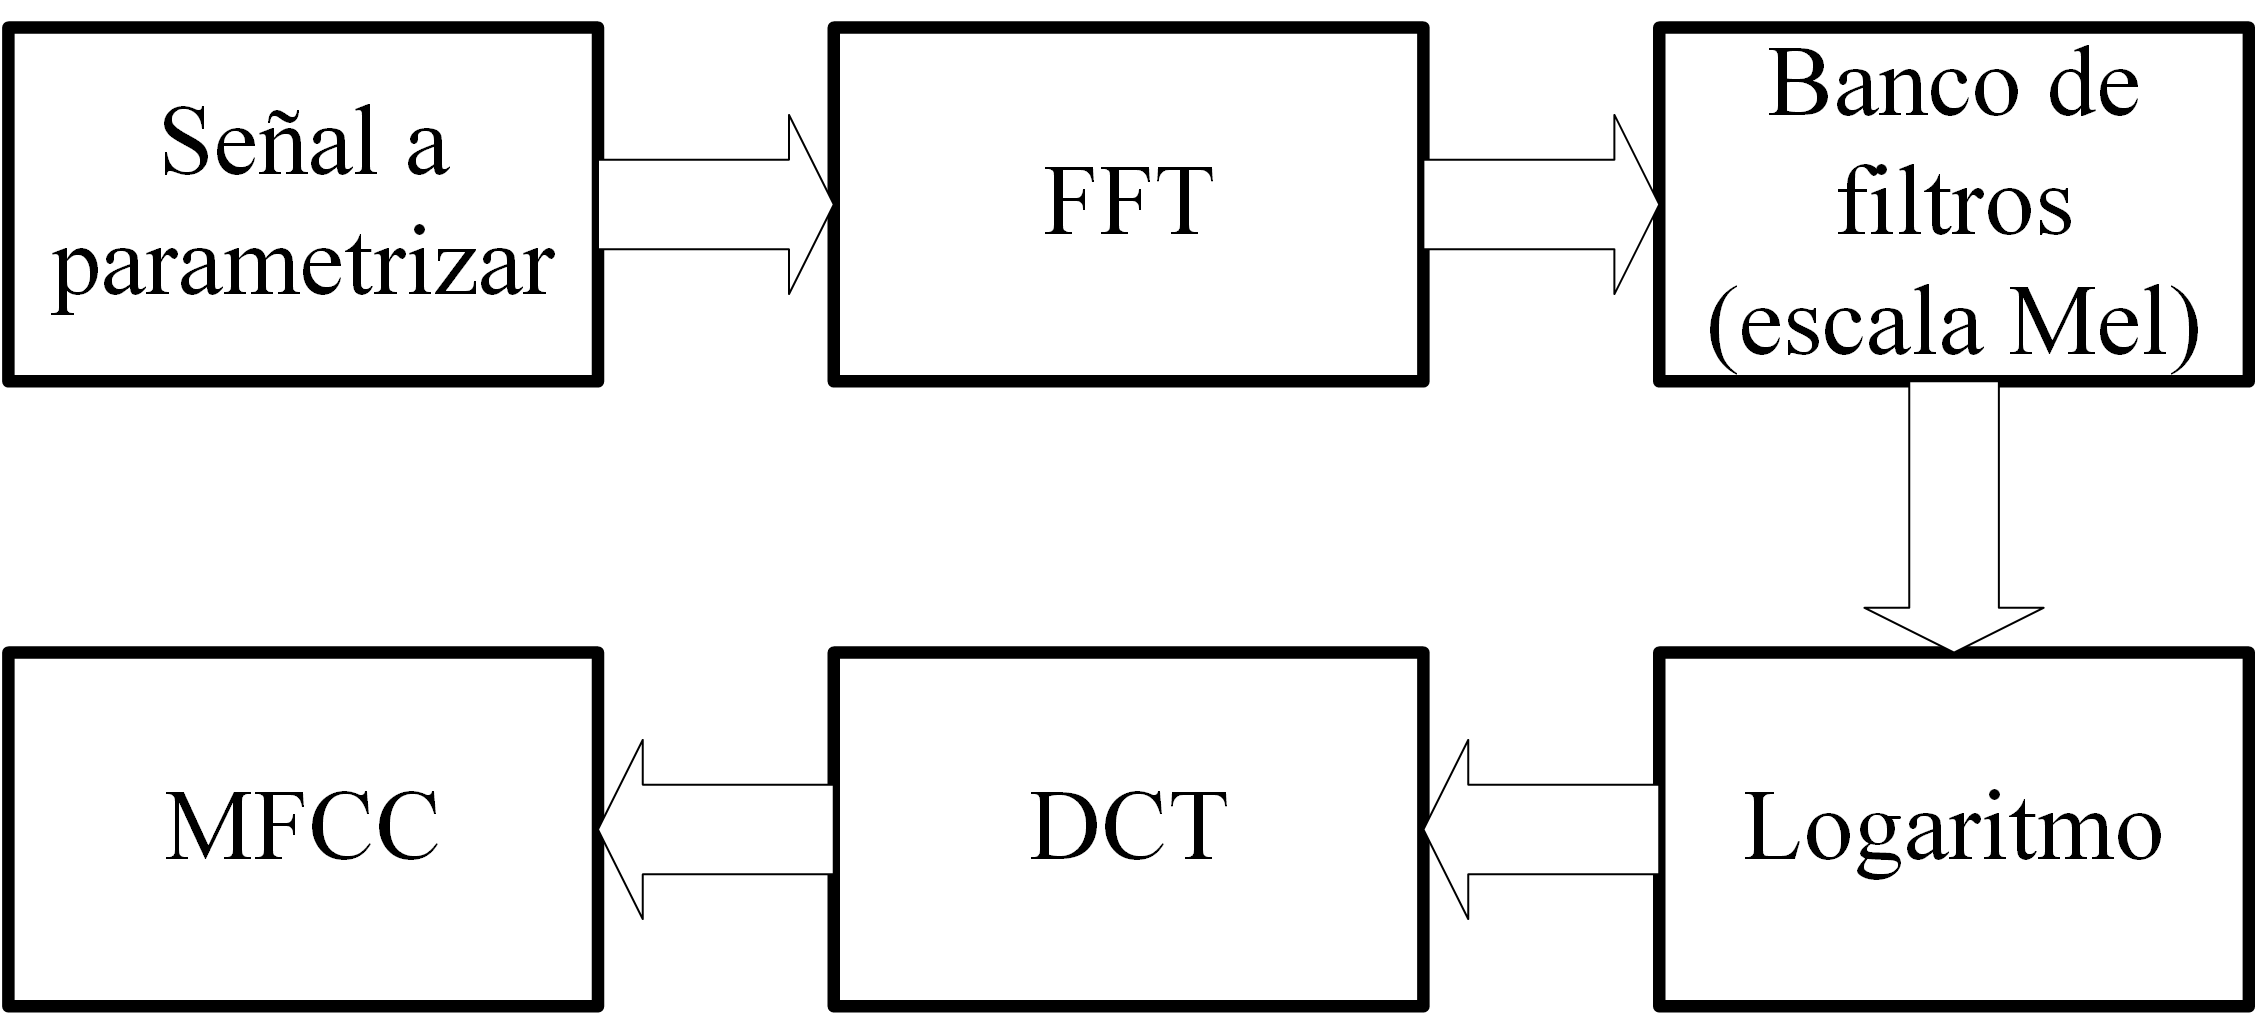
\includegraphics[width=0.6\linewidth]{figures/mfcc}
	\caption{Diagrama a bloques para el cálculo de MFCC}
	\label{fig:mfccB}
\end{figure}

\subsubsection*{FFT}

Se calcula la transformad de Fourier de Tiempo Corto a cada una de las tramas obtenidas de la etapa de pre-procesamiento mediante:

\begin{equation}\label{eq:fftCorto}
	x(n,\omega_k)=\sum_{m=-\infty}^{\infty}{x(m)\cdot w(n-m)\cdot e^{-j\omega_km}}
\end{equation}

Donde: $\omega_k=\frac{2\pi}{N}k$ 

\subsubsection*{Banco de filtros (escala Mel)}

Los filtros que se le aplican a la señal en la técnica MFCC están espaciados linealmente para frecuencias menores a 1000 Hz y logarítmicamente para frecuencias mayores de 1000 Hz. A esta escala se le denomina “Escala Mel” y su fórmula matemática está dada por la ecuación (\ref{eq:filtMEL}).

\begin{equation}\label{eq:filtMEL}
	Mel(f)=2595\cdot log(1+\frac{f}{700})
\end{equation}

El cuadrado de la magnitud de $x(n,\omega_k )$ es ponderado por una serie de filtros distribuidos sobre la escala de Mel para luego calcular la llamada energía del filtro l-ésimo mediante la ecuación (\ref{eq:logEnergia})

\begin{equation}\label{eq:logEnergia}
	E_{Mel}(n,l)=\frac{1}{A_l}\cdot \sum_{k=L_l}^{U_l}{|V_L(\omega_k)\cdot X(n,\omega_k)|^2}
\end{equation}

Donde $L_l$  y $U_l$ son las frecuencias de corte inferior y superior del filtro l-ésimo.

El banco de filtros linealmente espaciado en la escala de Mel tiene la forma que se muestra en la Figura 18 y los filtros que lo conforman pueden ser triangulares o tener otras formas, tales como Hamming, Hanning o kaizer, pero el triangular es el más utilizado.

\begin{figure}[H]
	\centering
	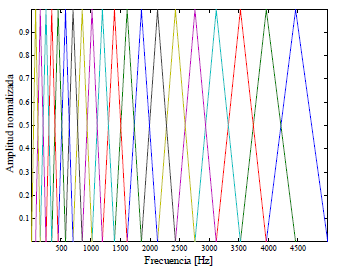
\includegraphics[width=0.6\linewidth]{figures/bancoFiltros}
	\caption{Banco de filtros en la escala de Mel}
	\label{fig:bancoFiltros}
\end{figure}

\subsubsection*{DCT}

Se convierte el espectro logarítmico Mel nuevamente al dominio del tiempo usando la Transformada Discreta del Coseno, dado que los coeficientes cepstrales son reales. El cálculo se realiza con la ecuación (\ref{eq:dct}).

\begin{equation}\label{eq:dct}
	C_{Mel}[n,m]=\frac{1}{R}\cdot \sum_{l=1}^{R}{log\left \{ E_{Mel}(n,l)\right \}\cdot cos[n(l-\frac{1}{2})\cdot \frac{\pi}{l}]}, n=1,2,3,...,K
\end{equation}

Donde K es el número de coeficientes cepstrales, que por lo general se escoge entre 10 y 20.

Mediante el proceso descrito, para cada trama de voz de duración aproximada igual a 30 ms con solapamiento, se calcula un conjunto de coeficientes cepstrales. Este es el resultado de la transformada Discreta de Coseno de la Densidad Espectral de Potencia expresada en la escala de Mel. A este conjunto de coeficientes se denomina Vector Acústico, por lo que cada entrada es transformada mediante este proceso en una secuencia de Vectores acústicos que representan las características más importantes de la voz, necesarias para el reconocimiento del habla. \cite{SalcedoCherubini2006}

\subsubsection{LFCC (Linear-Frequency Cepstral Coefficients)}

El funcionamiento de la obtención de los LFCC’s es similar al proceso de obtención de los MFCC’s, con la única diferencia de que los bancos de filtros utilizados que se le aplican a la señal se encuentran sobre una escala lineal. El banco de filtros que se generan con esta técnica se observa en la Figura \ref{fig:lfcc}.

\begin{figure}[H]
	\centering
	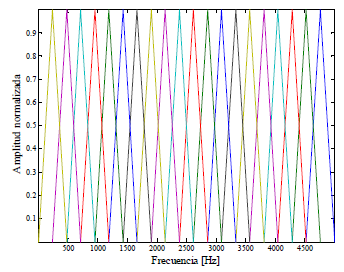
\includegraphics[width=0.6\linewidth]{figures/lfcc}
	\caption{Banco de filtros para el cálculo de LFCC's}
	\label{fig:lfcc}
\end{figure}

Cabe mencionar que la diferencia entre los tres métodos de extracción de características es principalmente que cada uno se utiliza para la extracción de distintas características de la voz.

\subsection{Cuantización vectorial}

El resultado de un análisis por banco de filtros o análisis LPC son una serie de vectores de las características espectrales variables en el tiempo de la señal de voz, donde típicamente cada vector es un vector p-dimensional. \cite{Rabiner1993}

Por esto, en particular para el reconocimiento del habla, la esencia de la cuantización vectorial es la de obtener a partir de un vector cualquiera de coeficientes cepstrales, un vector de tamaño fijo que se parezca lo más posible al original. Para ello, el espacio generado por los coeficientes cepstrales es dividido en un conjunto de regiones convexas mutuamente excluyentes y para cada una se calcula el centroide. El conjunto de centroide obtenidos de la partición del espacio generado por los coeficientes cepstrales se le denomina codebook. Por lo tanto, a cada palabra se la asocia su propio codebook.

La cuantización vectorial presenta ventajas y desventajas mencionadas en \cite{Rabiner1993}:

\begin{itemize}
\item	Ventajas
\begin{itemize}
\item	Reduce el almacenamiento de información de análisis espectral: La eficiencia de la representación de la cuantización vectorial puede ser explotada en sistemas de reconocimiento del habla.
\item	Reducción de cálculo para determinar la similitud de vectores de análisis espectral. En reconocimiento del habla un componente importante de la computación es la determinación de similitud espectral entre un par de vectores.  Basado en la representación de cuantización vectorial, este cálculo de similitud espectral es con frecuencia reducido a una búsqueda en la tabla de similitudes entre pares de vectores codebooks.
\item	Representación discreta de los sonidos del habla. Asociando una etiqueta fonética con cada vector codebook, el proceso de elegir el mejor vector codebook para representar un vector espectral dado llega a ser equivalente a asignar una etiqueta fonética a cada segmento espectral de voz. Existe una gama de sistemas de reconocimiento que explotan estas etiquetas con el fin de reconocer el habla de manera eficiente.
\end{itemize}
\item	Las desventajas de usar la cuantización vectorial para representar un vector espectral de voz son:
\begin{itemize}
\item	Una distorsión espectral inherente en la representación del vector de análisis actual. Ya que sólo hay un número finitos de vectores codebooks, el proceso de elegir la “mejor” representación de un vector espectral dado es equivalente a cuantizar el vector y conduce, por definición, a un cierto nivel de error de cuantización.
\item	El almacenamiento requerido por los vectores codebooks es con frecuencia no trivial. Cuanto más grande hacemos el codebook (con el fin de reducir el error de cuantización), más es el almacenamiento requerido para las entradas codebook.
\end{itemize}
\end{itemize}

\subsubsection{Elementos de la implementación de un cuantizador vectorial}

Para crear un cuantizador vectorial e implementar un procedimiento de análisis, necesitamos lo siguiente:

\begin{enumerate}
\item	Un gran conjunto de vectores de análisis espectral, que conforman el conjunto de entrenamiento. El conjunto de entrenamiento es usado para crear el “óptimo” conjunto de vectores codebook para representar la variabilidad espectral observada en el conjunto de entrenamiento. Si indicamos el tamaño de cuantizador vectorial como $M=2^B$ vectores (a esto se le llama un codebook de B bits), entonces requerimos $L>>M$ de manera que sea capaz de encontrar el mejor conjunto de M vectores codebook de manera robusta. En la práctica, se ha encontrado que L puede ser al menos 10M para que el entrenamiento del cuantizador vectorial trabaje razonablemente bien.
\item	Una mediad de similitud, o distancia, entre un par de vectores de análisis espectral de manera que sea capaz de agrupar el conjunto de vectores de entrenamiento, así como también asociar o clasificar arbitrariamente vectores espectrales en entradas únicas del codebook.
\item	Un procedimiento de cálculo de centroide. Sobre la base de la partición que clasifica los L conjuntos de vectores de entrenamiento en M grupos que, elegimos los M vectores codebook como el centroide de cada uno de los M grupos.
\item	Un procedimiento de clasificación de vectores de análisis de voz espectral arbitrarios que selecciona el vector codebook cercano al vector de entrada y usa el índice del codebook como resultado de representación espectral.
\end{enumerate}

La Figura \ref{fig:vectorQTS} muestra un diagrama de bloques del entrenamiento básico de un cuantificador vectorial y estructura de clasificación.

\begin{figure}[H]
	\centering
	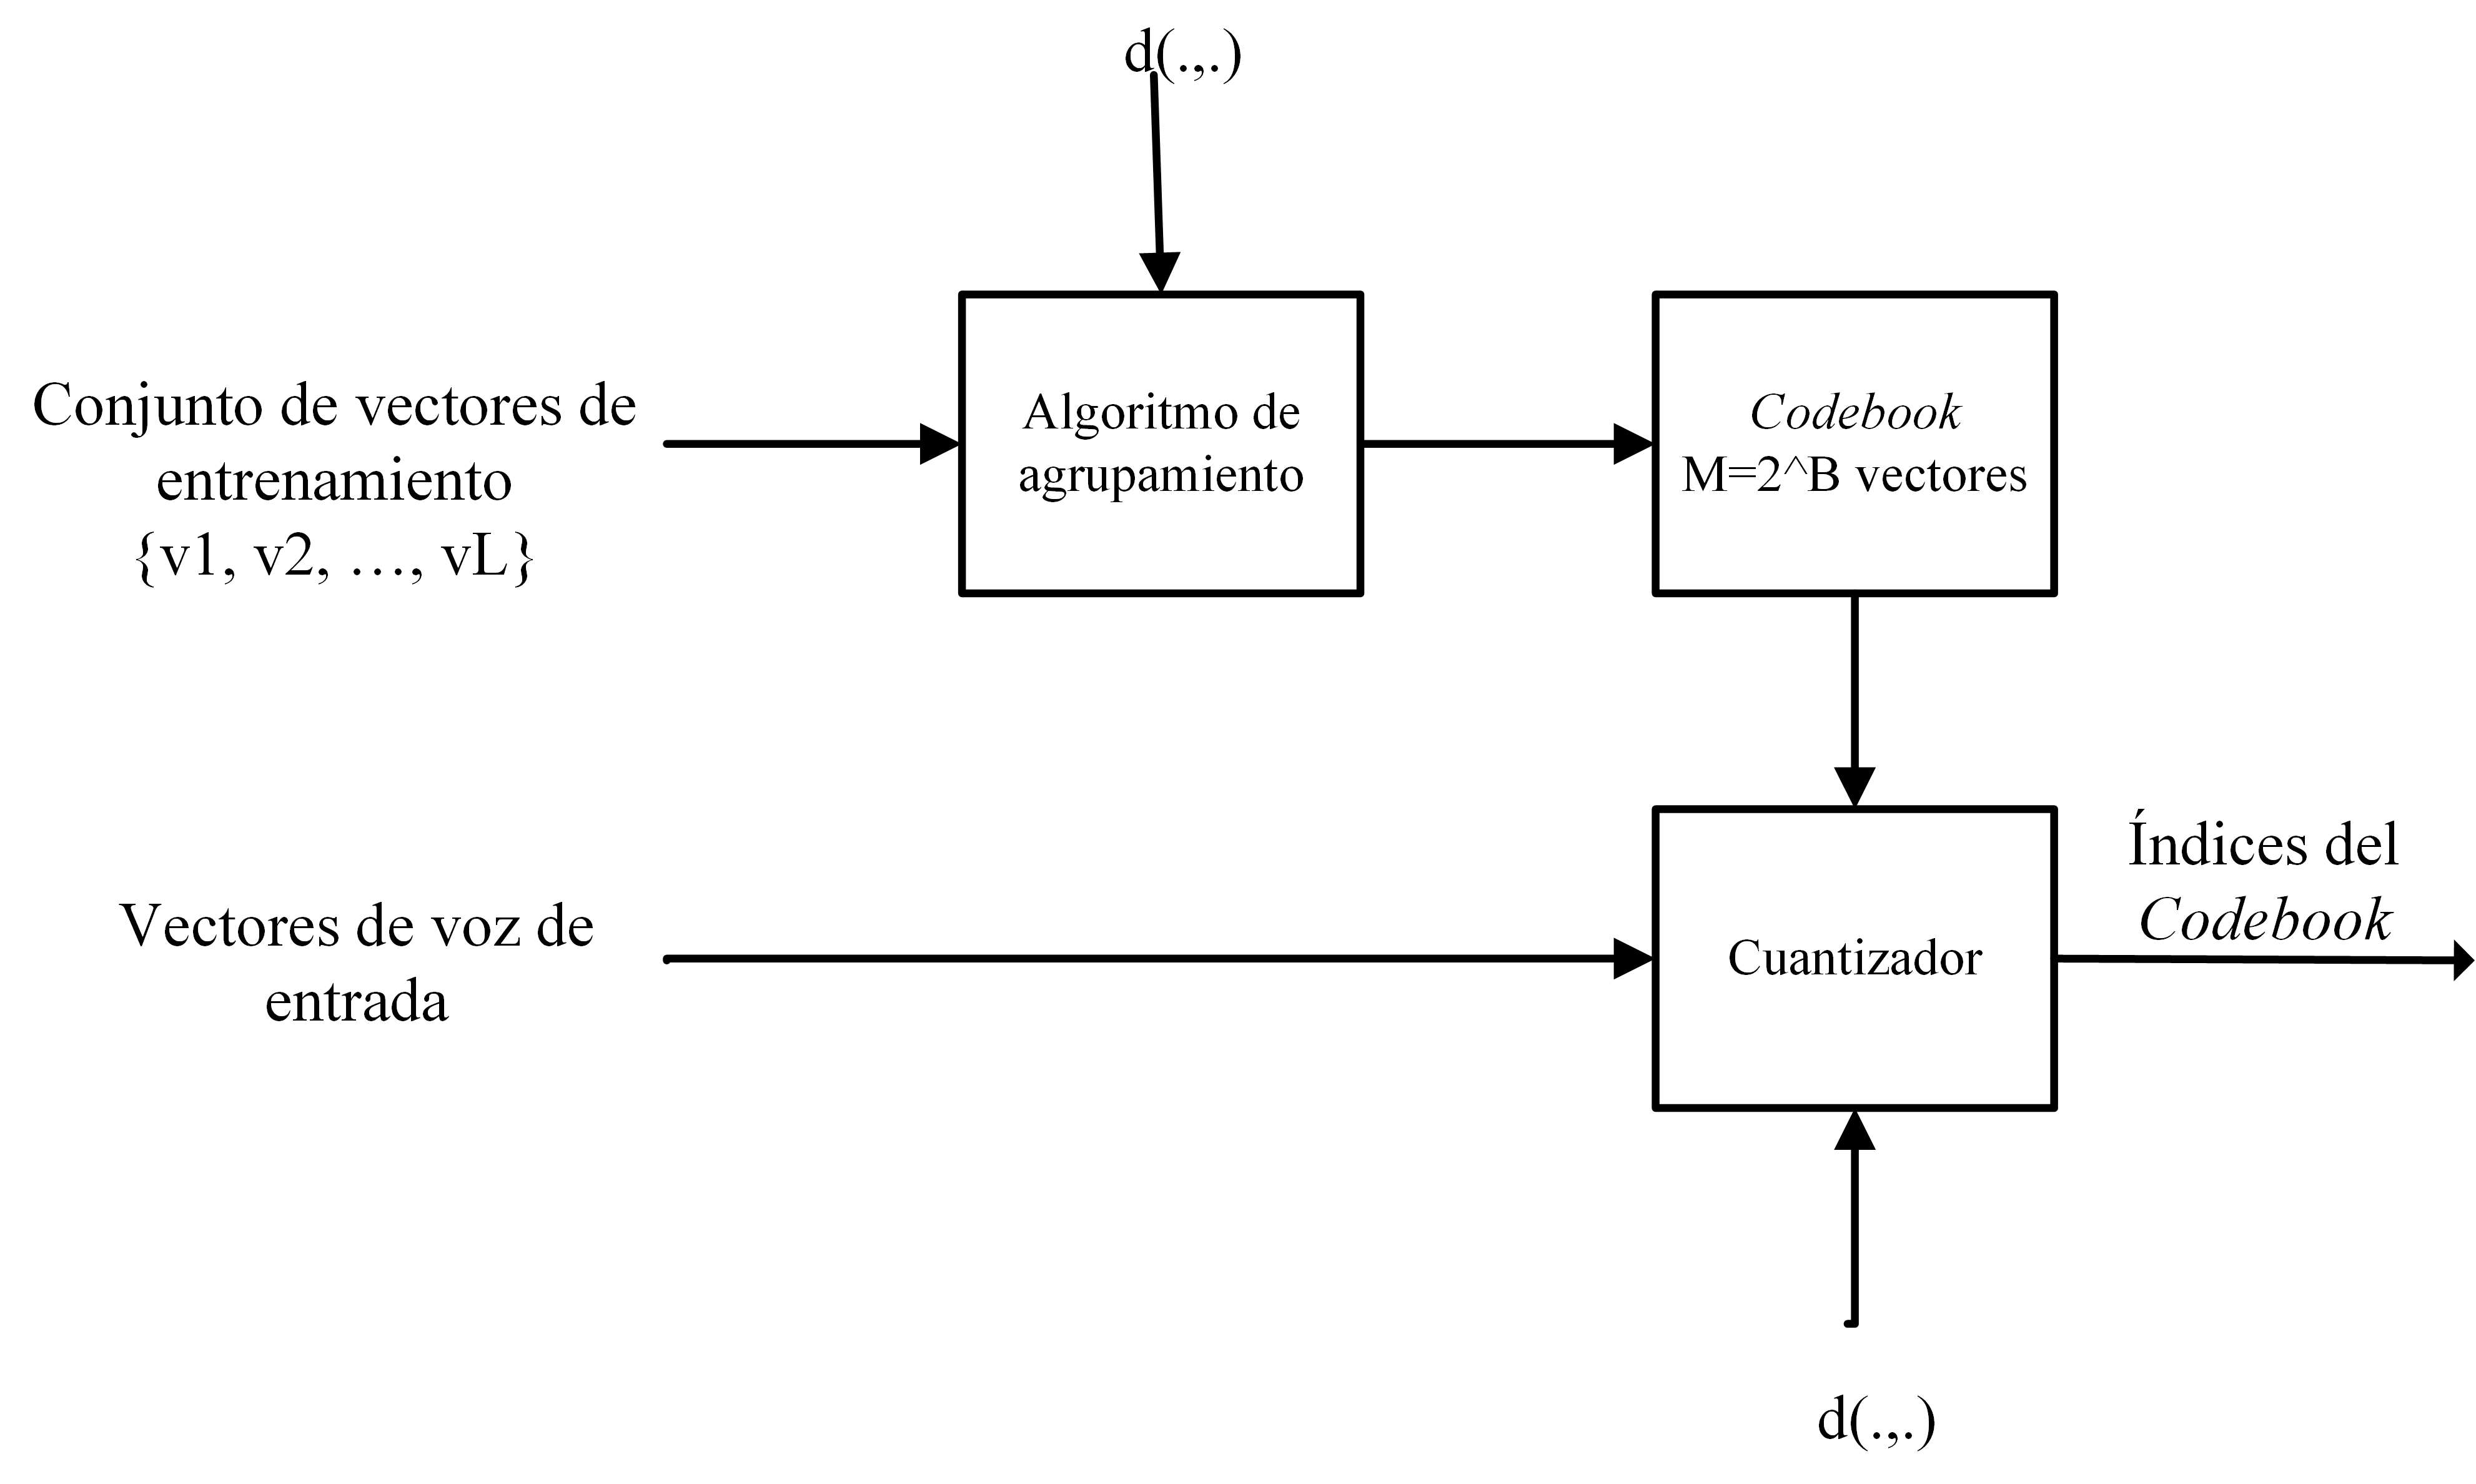
\includegraphics[width=0.6\linewidth]{figures/vectorQTS}
	\caption{Diagrama a bloques del entrenamiento básico de un cuantificador vectorial y estructura de clasificación}
	\label{fig:vectorQTS}
\end{figure}

\subsubsection{El conjunto de entrenamiento del cuantizador vectorial}

Para entrenar apropiadamente el \textit{codebook}, el conjunto de vectores de entrenamiento debe abarcar anticipadamente los siguientes puntos:

\begin{itemize}
\item	Interlocutores, incluyendo rangos de edad, acento, genero, velocidad de habla, nivel y otras variables.
\item	Condiciones de habla, tales como una habitación silenciosa, automovil, área de trabajo ruidosa.
\item	Transductores y sistemas de transmisión, incluyendo micrófonos de banda ancha, transmisión directa, canal telefónico, ancho de banda del canal y otros dispositivos.
\item	Fonemas, vocabulario de reconocimiento.
\end{itemize}

\subsubsection{Agrupación de los vectores de entrenamiento.}

La manera en que el conjunto de L vectores de entrenamiento puede ser agrupados en un conjunto de M vectores codebook es el siguiente (este procedimiento es conocido como el algoritmo generalizado de Lloyd o el algoritmo de agrupación K-means):

\begin{enumerate}
\item	Inicialización: Arbitrariamente elige M vectores (inicialmente fuera del conjunto de entrenamiento de L vectores) como el conjunto inicial de codewords en el codebook.
\item	Buscar el vecino más cercano: Para cada vector de entrenamiento encontrar el codeword en el actual codebook más cercano (en términos de distancia espectral), y asigna ese vector a la celda correspondiente (asociada con el codeword más cercano).
\item	Actualiza el centroide: Actualiza el codeword en cada celda usando el centroide del vector de entrenamiento asignado a esa celda.
\item	Iteración: Repetir paso 2 y 3 hasta que la distancia media cae por debajo del presente umbral.
\end{enumerate}

La Figura \ref{fig:partitioningVectorSpace} ilustra el resultado del diseño de el \textit{codebook} mostrando la partición del espacio vectorial espectral en distintas regiones, cada uno representado por el centroide del vector

\begin{figure}[H]
	\centering
	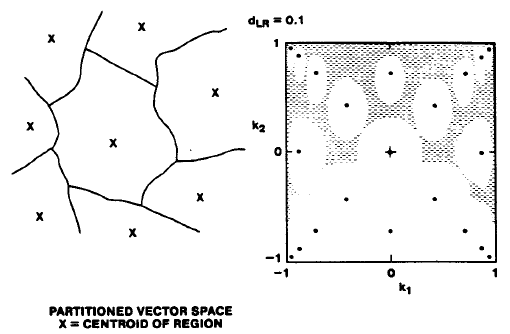
\includegraphics[width=0.6\linewidth]{figures/partitioningVectorSpace}
	\caption{Partición de un espacio vectorial en celdas de cuantización vectorial con cada celda representada por el centroide del vector}
	\label{fig:partitioningVectorSpace}
\end{figure}
	
Aunque el procedimiento iterativo mostrado funciona correctamente, ha sido demostrado que es ventajoso diseñar un codebook de M vectores en etapas, por ejemplo, primero diseñando un codebook de 1 vector, entonces usar la técnica de división en el codeword para inicializar la búsqueda de un codebook de 2 vectores, y continuar con el proceso de división hasta el deseado codebook de M vectores. Este procedimiento es llamado el algoritmo de división binaria y es formalmente implementado mediante el siguiente procedimiento.
	
\begin{enumerate}
\item	Diseñar un vector genérico del codebook; éste será el centroide del conjunto entero de vectores de entrenamiento.
\item	Duplicar el tamaño del codebook dividiendo cada codebook existente $y_n$ de acuerdo a la regla

\begin{equation}\label{eq:codebook}
	\begin{cases}
	    y_n^+=y_n(1+\epsilon)\\
			    y_n^-=y_n(1-\epsilon)
\end{cases}
\end{equation}

Donde n varía de 1 al tamaño actual del codebook, y $\epsilon$ es un parámetro de separación (típicamente $\epsilon$ es elegido en el rango $0.01\leq \epsilon \leq 0.05$).
\item	Usar el algoritmo de iteración K-means para conseguir el mejor conjunto de centroides para la división del codebook.
\item	Iterar los pasos 2 y 3 hasta que el codebook de tamaño M esté diseñado.
\end{enumerate}

\subsection{Redes Neuronales Artificiales}

		\subsubsection{Modelo de neurona artificial}

		Las redes neuronales artificiales pretenden emular la red neuronal biológica y se obtiene interconectando neuronas. Para ello se supone un modelo matemático simplificado de la neurona biológica \cite{Faundez2001}.
		
		Este modelo es una generalización del propuesto por McCulloch y Pitts en 1943:

		\begin{equation}\label{eq:ej}
			y = f \left[ \left( \sum_{i=1}^{N}\omega_i*x\left(n-i\right)\right)-b	\right]
		\end{equation}		

		La Figura \ref{fig:neuronaModel} representa el modelo de neurona artificial.

		\begin{figure}[H]
			\centering
			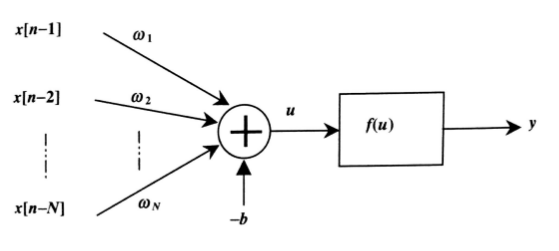
\includegraphics[width=0.6\linewidth]{figures/neuronaA}
			\caption{Modelo de neurona artificial.}
			\label{fig:neuronaModel}
		\end{figure}		

		La neurona recibe del exterior un umbral b y N entradas a las que asocia un conjunto de pesos $\omega_i(i=1,..., N)$. Aplicando el producto de los pesos por las entradas respectivas más el umbral (o desplazamiento) a una función de activación $f(u)$, se obtiene la salida $y$\cite{Faundez2001}.

		$u(\vec{x},\vec{\omega})$ recibe el nombre de función base, donde los vectores $\vec{x}$, $\vec{\omega}$ son:

		\begin{equation}\label{eq:ej}
			\vec{x}=\left\{ x\left[n-1\right],..., \left[n-N\right]	\right\}
		\end{equation}		

		\begin{equation}\label{eq:ej}
			\vec{\omega}=\left\{ \omega_1,..., \omega_N	\right\}
		\end{equation}		

		Cuando la combinación de las entradas es de tipo lineal, $u(\vec{x},\vec{\omega})$ es una función de base lineal, pero son posibles otras combinaciones, entre las que destacan las funciones de base radial, consistentes en realizar una operación no lineal sobre las entradas, con simetría radial. Por ejemplo:

		\begin{equation}\label{eq:ej}
			u\left(\vec{x},\vec{\omega}\right)=\sum_{i=1}^{N}\left[\omega_i-x\left(n-i\right)\right]^2
		\end{equation}		


		La función de activación es la encargada de tomar la decisión de cuándo está activada la neurona y cuándo no, las funciones de activación más comunes se muestran en la Figura \ref{fig:funcionesAct}.

		\begin{figure}[H]
			\centering
			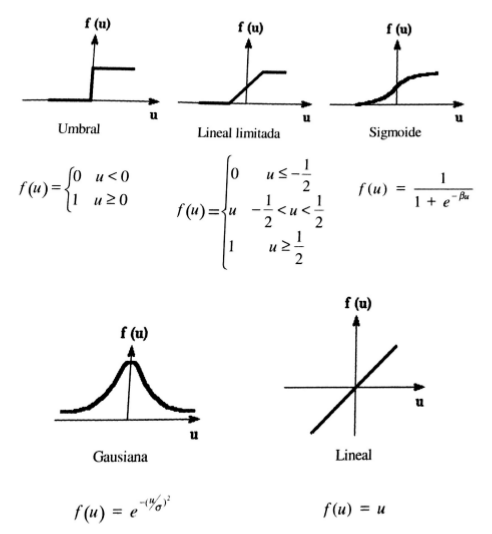
\includegraphics[width=0.6\linewidth]{figures/funcionesAct}
			\caption{Funciones de activación.}
			\label{fig:funcionesAct}
		\end{figure}		

		\subsubsection{Arquitectura de una Red Neuronal Artificial (RNA)}

		Las neuronas de una determinada red pertenecerán a una de las siguientes clases:

		\begin{itemize}
			\item \textbf{Neuronas de entrada:} Reciben las señales exteriores. Integran la primera capa de red.
			\item \textbf{Neuronas ocultas:} Producen resultados intermedios.
			\item \textbf{Neuronas de salida:} Su salida es observable desde el exterior. Constituyen la última capa de la red.
		\end{itemize}

		Por otra parte, dependiendo de la forma en que se encuentren las neuronas y sus conexiones, aparecen dos grandes tipos de redes:
	
		\begin{itemize}
			\item Redes progresivas.
			\item Redes realimentadas.
		\end{itemize}

		En las \textbf{redes progresivas} las conexiones de sus neuronas (y, por lo tanto, el flujo de información) son siempre hacia adelante, de la entrada a la salida. No presentan memoria. Por tanto, son estáticas.

		Las arquitecturas progresivas de mayor importancia son el \textsl{perceptrón} y las redes de función de base radial.

		\begin{figure}[H]
			\centering
			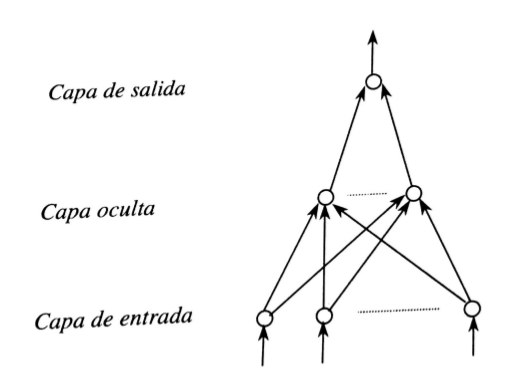
\includegraphics[width=0.8\linewidth]{figures/redProgresiva}
			\caption{Red progresiva.}
			\label{fig:redProgresiva}
		\end{figure}	

		A diferencia de las redes progresivas, las \textbf{redes realimentadas} presentan como mínimo un camino de realimentación, ya sea entre neuronas de una misma capa (conexiones laterales) o como conexión hacia atrás, de una capa exterior a una más interior.

		Son sistemas dinámicos. Cada vez que se presenta una nueva entrada a la red, se calcula la salida de las neuronas. Debido a los lazos de realimentación, las entradas de las neuronas se modifican y la red entra en un nuevo estado \cite{Faundez2001}.

		Las arquitecturas más destacables son:

		\begin{itemize}
			\item Redes competitivas.
			\item Mapas auto organizados de Kohonen.
			\item Red de Hopfield.
			\item Red de Elmann.
			\item Modelos ART.
		\end{itemize}

		\begin{figure}[H]
			\centering
			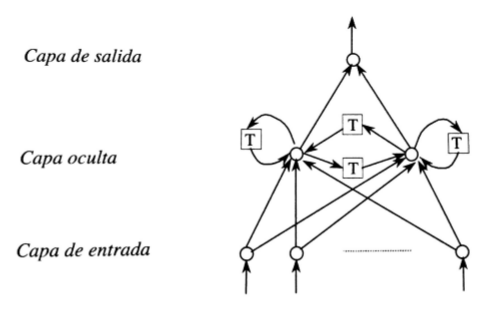
\includegraphics[width=0.8\linewidth]{figures/redRealimentada}
			\caption{Red realimentada.}
			\label{fig:redRealimentada}
		\end{figure}	

		\subsubsection{Aprendizaje}

		Una vez que se establece la arquitectura y el número de neuronas de la red, hay que calcular el valor de los pesos para que realice la función deseada. Usualmente, la red debe aprender el peso de las conexiones a partir de un conjunto de patrones de entrenamiento. Por tanto, no se calculan los pesos de forma analítica, sino que es necesario un proceso de aprendizaje automático  partir de una serie de ejemplos.

		Para diseñar un proceso de aprendizaje será necesario disponer de:

		\begin{itemize}
			\item Un conjunto de información disponible para el aprendizaje.
			\item Un proceso para actualizar los pesos, o algoritmo de aprendizaje.
		\end{itemize}

		\textbf{Aprendizaje supervisado:}
		La red conoce la salida correcta para cada patrón de entrada. Por tanto, se ajustan los pesos de forma que las salidas de la red sean lo más parecidas posibles a la salida correcta.

		\textbf{Aprendizaje por refuerzo:}
		Es una variante del método anterior, en el cual la red únicamente conoce una crítica sobre la exactitud de las salidas, pero no la respuesta correcta.

		Utiliza un mecanismo de penalización y recompensa, mediante el cual la red resulta recompensada por una decisión correcta y castigada por una equivocada. De esta forma, el sistema tiende a actuar de la forma favorecida y debilita la tendencia a proporcionar la respuesta penalizada.

		\textbf{Aprendizaje auto organizado:}
		No requiere el conocimiento de la salida correcta, y debe aprender la estructura implícita en los datos. Generalmente requiere un número mayor de datos de entrenamiento.

		\paragraph{}
		En el aprendizaje, existen tres cuestiones importantes:
		
		\textbf{Capacidad de la red para implementar funciones y aprender patrones.}
		Dependerá de su estructura, tamaño, etc.

		\textbf{Complejidad de los datos.}
		Determina el número de patrones de entrenamiento necesarios para entrenar la red de forma que se garantice una buena capacidad de generalización (capacidad de procesar correctamente datos no utilizados en el aprendizaje). Si el número de patrones es pequeño, la red se comportará bien con aquellos patrones utilizados en el entrenamiento, pero presentará un comportamiento pobre con aquellos datos no utilizados.

		\textbf{Complejidad computacional.}
		Condiciona el tiempo necesario para que el algoritmo de aprendizaje proporcione una solución ajustada.

		El conjunto de patrones utilizados en el proceso de aprendizaje recibe el nombre de secuencia de entrenamiento. Cada vez que se ha presentado la totalidad de la secuencia de entrenamiento a la red, se dice que se ha realizado un ``epoch". Normalmente los algoritmos que consumen poco tiempo en cada epoch requieren muchas epochs y viceversa, con lo cual la evaluación de la complejidad computacional debe considerar el número de epochs necesarios y el tiempo transcurrido en cada epoch \cite{Faundez2001}.

		En la tabla \ref{tabla:aprendizaje} se observan los 3 paradigmas de aprendizaje con sus reglas, arquitectura, algoritmo y tareas correspondientes.

		\begin{table}[H]
			\centering
			\begin{tabular}{| c | p{3cm} | p{3cm} | p{3cm} | p{3cm} |}
				\hline
				\multicolumn{5}{|c|}{Algoritmos de aprendizaje más conocidos} \\
				\hline
				Paradigma	&	Regla de aprendizaje	&	Arquitectura	&	Algortimo de aprendizaje	&	Tareas \\
				\hline \hline
				Supervisado	&	Corrección del error	&	Perceptrón o perceptrón multicapa	&	Algoritmos de aprendizaje perceptrón, retropropagación del error, ADALINE, MADALINE	&	Clasificación de patrones, aproximación de funciones, predicción, control, ... \\

				&	&	Elman y Jordan recurrentes	&	Retropropagación del error	&	Síntesis de series temporales\\

			&	Boltzmann	&	Recurrente	&	Algortimo de aprendizaje Boltzmann	&	Clasificación de patrones\\

			&	Competitivo	&	Competitivo	&	LVQ	&	Categorización intra-clase, comprensión de datos\\
			
			&	&	Red ART	&	ARTMap	&	Clasificación de patrones, categorización intra-clase\\
			\hline

			No Supervisado	&	Corrección del error	&	Red de Hopfield	&	Aprendizaje de memoria asociativa	&	Memoria asociativa\\
			&	&	Multicapa sin realimentación	&	Proyección de Sannon	&	Análisis de datos\\

			&	Competitiva	&	Competitiva	&	VQ	&	Categorización, compresión de datos\\

			&	&	SOM	&	Kohonen SOM	&	Categorización, análisis de datos\\

			&	&	Redes ART	&	ART1, ART2	&	Categorización\\
			\hline

			Por refuerzo	&	Hebbian	&	Multicapa sin realimentación	&	Análisis lineal de discriminante	&	Análisis de datos, clasificación de patrones\\

			&	&	Sin realimentación o competitiva	&	Análisis de componentes principales	&	Análisis de datos, compresión de datos\\
			\hline
			\end{tabular}
			\caption{Algoritmos de aprendizaje más conocidos.}
			\label{tabla:aprendizaje}
		\end{table}

		\subsubsection{Aplicaciones de las RNA}

		Las principales aplicaciones de las rede neuronales aplicadas al tratamiento de voz e imagen se pueden dividir en:
		\begin{itemize}
			\item\textbf{Clasificación de patrones}

			Consiste en asignar un patrón de entrada, representado normalmente por un vector de características a una de las clases predeterminada. Las principales aplicaciones en las que las redes neuronales actúan de forma satisfactoria como clasificadores son: reconocimiento de caracteres, del habla y de locutor.
			\item \textbf{Agrupaciones (clustering)}

			También se conoce como clasificación no supervisada de patrones. El algoritmo examina la semejanza entre patrones, y los agrupa en un cierto número de clases. Tiene aplicación en compresión de datos y como paso preliminar en aplicaciones de reconocimiento.
			\item \textbf{Aproximación de funciones}

			A partir de un conjunto finito de patrones se encuentra una función interpolativa que permite calcular la salida a entradas nuevas. Es una alternativa a los métodos de interpolación clásicos, con la ventaja de obtener fácilmente una función de interpolación no lineal. Es útil en voz e imagen para la interpolación de señal, parámetros, etc.
			\item \textbf{Predicción}

			Dado un conjunto de muestras de entrada hasta un determinado instante de tiempo, se pretende predecir la muestra siguiente en un tiempo futuro. La obtención de modelos predictivos para una determinada señal es ampliamente utilizada en tratamiento de voz e imagen en todos sus campos.

			Destaca especialmente la predicción no lineal basada en red neuronal, por sus mayores prestaciones respecto a los métodos lineales \cite{Faundez2001}.
		\end{itemize}

		\subsubsection{Ejemplos de aplicación}

		Como se mencionó, las redes neuronales tienen diversas aplicaciones, en \cite{LunaMoreno2001} se usa una red neuronal perceptrón multi-capa para realizar la clasificación de marcos de tiempo por categorías fonéticas, en este trabajo se usan 130 nodos de entrada los cuales están compuestos por 5 frames de 26 características delta cada uno, consta de 200 nodos escondidos y 545 nodos de salida, que corresponden a los 544 categorías basadas fonéticamente.

		Otro ejemplo se presenta en \cite{CruzBeltran}, en este trabajo se usa una red neuronal backpropagation, este trabajo consiste en el reconocimiento de locutores y se hace uso de 25 nodos en la capa de entrada, 21 nodos en la capa oculta y 5 nodos en la capa de salida, los datos ingresados en la capa de entrada son las características espectrales dadas por el extractor de características y la salida se representa como una salida binaria, donde cada nodo representa un locutor y sólo se activa el nodo del locutor reconocido.

		En \cite{RasconMontiel2009} se presenta el reconocimiento de voz mediante una red  neuronal de retropropagación para el reconocimiento de dos personas usando 11 neuronas en la capa de entrada, 7 en a capa oculta y 3 en la capa de salida y en \cite{Fernandez} se presenta el reconocimiento de voz mediante una red neuronal de Kohonen y se opta en este trabajo el uso de 100 neuronas para evitar los largos procesos de entrenamiento, principalmente se hace el reconocimiento de la pronunciación de los números del cero al nueve.

		\subsection{Bases de datos}

		Una base de datos (BD) es una entidad en la cual se pueden almacenar datos de manera estructurada, con la menor redundancia posible. Diferentes programas y diferentes usuarios deben poder utilizar estos datos. Por lo tanto, el concepto de base de datos generalmente está relacionado con el de red ya que se debe poder compartir esta información.

		Una base de datos proporciona a los usuarios el acceso a datos, que pueden visualizar, ingresar o actualizar, en concordancia con los derechos de acceso que se les haya otorgado.

		La principal ventaja de utilizar bases de datos es que múltiples usuarios pueden acceder a ellas al mismo tiempo \cite{BD2015}.

		Un sistema de administración de bases de datos (Data Base Manager System, DBMS), es aquel que controla la organización, almacenamiento, recuperación, seguridad e integridad de los datos en una base de datos. En la tabla \ref{tabla:dbms} se hace la comparación de algunas características importantes de los tres principales DBMS que son SQL server, PostgreSQL y MySQL de los datos obtenidos en \cite{Hsu2008} y \cite{dbms}.

		\begin{table}[H]
			\centering
			\begin{tabular}{| p{4cm} | p{3.5cm} | p{3.5cm} | p{3.5cm} |}
				\hline
				\multicolumn{4}{|c|}{DBMS más utilizados} \\
				\hline
				Característica	&	Microsoft SQL Server	&	MySQL	&	PostgreSQL\\
				\hline \hline

				Modelode base de datos	&	DBMS Relacional	&	DBMS Relacional	&	DBMS Relacional\\
			\hline

				Licencia	&	Comercial, Closed Source, varios niveles de características basado en la versión	&	GPL Open Source y comercial	&	BSD Open Source\\
			\hline

				Proceso de instalación y mantenimiento	&	Difícil y consume gran cantidad de recursos	&	Fácil	&	Medio\\
			\hline

				Controladores ODBC, JDBC, ADO.NET disponibles	&	Sí	&	Sí	&	Sí\\
			\hline

				Lenguaje de implementación	&	C++	&	C y C++	&	C\\
			\hline
				Sistema operativo del servidor	&	Windows	&	FreeBSD, Linux, OS X, Solaris, Windows	&	FreeBSD, HP-UX, Linux, NetBSD, OpenBSD, OS X, Solaris, Unix, Windows\\
			\hline
			\end{tabular}
			\caption{Comparación de DBMS más utilizados.}
			\label{tabla:dbms}
		\end{table}

		\subsection{Android}

		Android es un sistema operativo inicialmente pensado para teléfonos móviles, al igual que iOS, Symbian y Blackberry OS. Lo que lo hace diferente es que está basado en Linux, un núcleo de sistema operativo libre, gratuito y multiplataforma.

		El sistema permite programa aplicaciones en una variación de Java llamada Dalvik. El sistema operativo proporcionar todas las interfaces necesarias para desarrollar aplicaciones que accedan a las funciones del teléfono (como el GPS, las llamadas, la agenda, etc.) de una forma muy sencilla en un lenguaje de programación muy conocido como es Java.

		Una de las mejores características de este sistema operativo es que es completamente libre. Es decir, ni para programar en este sistema ni para incluirlo en un teléfono hay que pagar nada. Y esto lo hace muy popular entre fabricantes y desarrolladores, ya que los costes para lanzar un teléfono o una aplicación son muy bajos \cite{Nieto2011}.

		\subsection{Motor de síntesis de voz de Google}

		El motor de síntesis de voz de google permite que las aplicaciones lean en voz alta el texto que aparece en pantalla. Algunas de las aplicaciones que pueden utilizarlo son:
	
		\begin{itemize}
			\item Google Play Libros para utilizar la función Leer en voz alta.
			\item El traductor de google para oir cómo se pronuncia una palabra.
			\item TalkBack y aplicaciones de accesibilidad.
			\item Muchas otras aplicaciones.
		\end{itemize}

		La aplicación se encuentra disponible para dispositivos con Android 4.0.3 o superior y cuenta con los idiomas alemán, coreano, español, frances, inglés (Estados Unidos), inglés (Reino Unido) e italiano.
		
		\subsection{Web Service}
		
		Un web service es un conjunto de protocolos y estándares que sirven para intercambiar datos entre aplicaciones. Distintas aplicaciones de software desarrolladas en lenguajes de programación diferentes, y ejecutadas sobre cualquier plataforma, pueden utilizar los servicios web para intercambiar datos en redes de ordenadores como internet.

De una manera más clara se podría decir que un web service es una función que diferentes servicios o equipos utilizan; es decir, solo se envían parámetros al servidor (lugar donde está alojado el web service) y éste responderá la petición. \cite{webservice}

\section{Análisis}

En esta sección se muestra el análisis de las técnicas empleadas para el reconocimiento de voz, la implementación y diversas pruebas para la elección del sistema propuesto.

\subsection{Del reconocimiento de voz}

	El análisis y elección de técnicas para la etapa de reconocimiento se hacen con base al estado del arte presentado en este documento.
	
	Como se vio en la sección \ref{sub:sr} los artículos \cite{A30}, \cite{A31}, \cite{A6} y \cite{A7} mencionan explicitamente algunas de las características de la voz para que esté adecuada a la etapa de reconocimiento. En general el pre-procesamiento de la señal de voz se lleva a cabo de acuerdo al bloque mostrado en la Figura \ref{fig:ana:prepro}.
	
		\begin{figure}[H]
			\centering
			
\includegraphics[width=1\linewidth]{figures/analisispreproce}
			\caption{Diagrama de la etapa de pre-procesamiento.}
			\label{fig:ana:prepro}
		\end{figure}
		
	De acuerdo a la Figura \ref{fig:ana:prepro} obtenemos las siguientes etapas a seguir:
	
	\subsubsection*{Digitalización}
	
	La digitalización es el primer proceso que se llevará a cabo y será la conversión de la señal de voz analógica a digital, esto a través del micrófono del dispositivo móvil. Para este proceso se decide utilizar una frecuencia de muestreo de 8 kHz y un tamaño de muestra de 8 bits, esto con el fin de optimizar los recursos del teléfono móvil. Dados los alcances presentados la duración máxima de la grabación de voz será de 10 segundos, por lo que la memoria máxima que ocupará un mensaje de voz será de $memoria=(8000\frac{muestras}{segundo}\cdot 10 segundos\cdot 8\frac{bits}{muestra}=640000 bits = 78.125 kB$, por lo que en una conectividad 4G con una velocidad de subida de 50Mbps, la señal de voz con mayor duración tardará 12.8 ms en ser enviada al servidor.
	
	\subsubsection*{Preénfasis}
	
	Como se vio en la sección del estado del arte, diversos artículos aplican el filtro preénfasis para resaltar características de la señal de voz, para esto se usa la fórmula $\hat{s}(n)=s(n)-a\cdot s(n-1)$, el valor de $a$ que se usará es el propuesto en \cite{A6} que es de $a=0.95$, en la Figura \ref{fig:ana:preenfasis} se muestra la aplicación del filtro a una señal de voz, así como también su espectro correspondiente, en éstos podemos observar cómo el espectro correspondiente a la señal filtrada se ve aplanado, de esta forma se pueden apreciar con mayor medida los formantes de la señal, para este caso, el interlocutor es una mujer de 22 años, y de acuerdo a la teoría, la frecuencia fundamental para las mujeres se encuentra entre los 200 y 250 Hz, en este caso lo podemos ubicar en los 200 Hz.
	
		\begin{figure}[H]
			\centering
			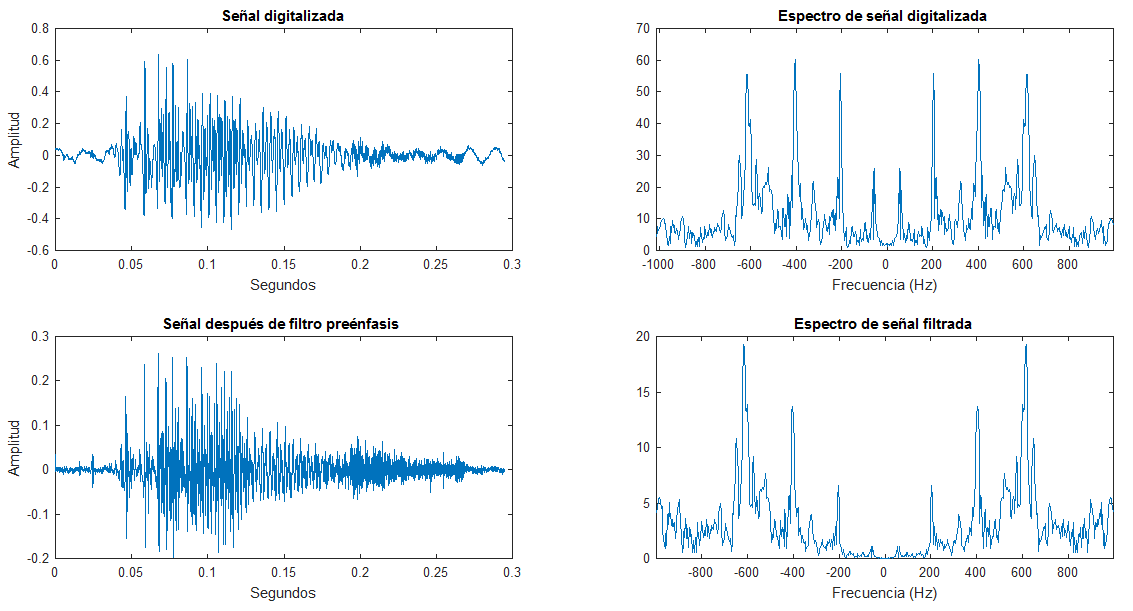
\includegraphics[width=1\linewidth]{figures/preenfasis}
			\caption{Aplicación del filtro de preénfasis.}
			\label{fig:ana:preenfasis}
		\end{figure}
	
	\subsubsection*{Detección de inicio y final de las palabras}
	
	Para la detección de bordes de palabras aisladas Rabiner en \cite{Rabiner1975} propone un algoritmo que hace uso de la energía de la señal y la tasa de cruces por cero y \cite{A31} por otro lado, propone el uso de la energía de la señal y la tasa de cruces por cero en tiempo corto, además de dos características en el dominio de la frecuencia, que son el centroide y flujo espectral, debido a los resultados de 96.25\% de éxitos en la segmentación de \cite{A31} se haría uso de este algoritmo de umbral dinámico para llevar a cabo la segmentación de las palabras de la frase a reconocer, sin embargo, tomando en cuenta que el tiempo de respuesta del sistema debe ser adecuada para llevar a cabo una conversación fluida y con esto que la experiencia de usuario no se vea afectada se decide hacer uso de la energía y tasa de cruces por cero para llevar a cabo la detección de bordes de la palabra y de esta forma llevar a cabo su separación. 
	
	\subsubsection*{Segmentación y aplicación de la ventana}
	
	La segmentación se lleva a cabo para que la señal de voz sea tratada como una señal estacionaria, la longitud del segmento que se propone en \cite{A6}, que corresponde a 45 ms del segmento con un espaciado de 15 ms y un traslape de 30 ms presentan buenos resultados, sin embargo, dados los tiempos de respuesta, esto implica llevar un mayor procesamiento, por lo que se proponen segmentos de 40 ms de duración y un traslape del 50\%. La ventana que será aplicada es la ventana de Hamming, esto debido a que la mayoría de los artículos la usa y como se mencionó en el marco teórico es la ventana que guarda la mejor relación de lóbulo central y laterales. En la Figura \ref{fig:ana:windowing} se puede observar uno de estos segmentos de la señal de voz con la ventana Hamming aplicada, es apreciable el amortiguamiento que genera la ventana y la periodicidad que obtiene la señal gracias a la segmentación.
	
	 \begin{figure}[H]
			\centering
			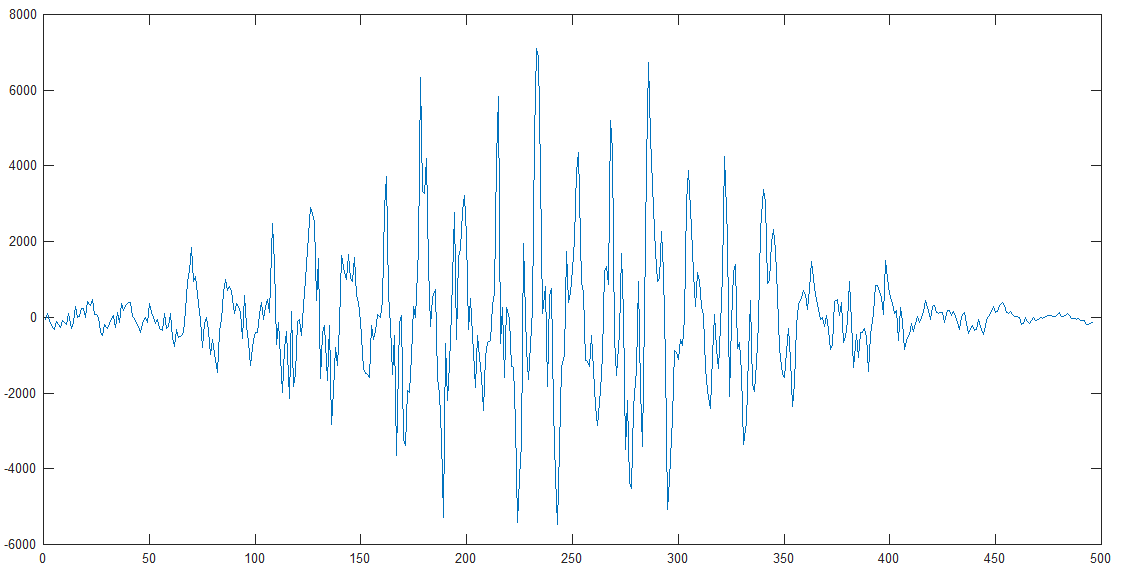
\includegraphics[width=0.8\linewidth]{figures/windowing}
			\caption{Segmentación y ventaneo de la señal de voz.}
			\label{fig:ana:windowing}
	\end{figure}
	
	\subsubsection*{Extracción de características}
	
	La siguiente fase es la extracción de características, de acuerdo a \cite{A1} el estado del arte de extracción de características es la técnica MFCC ya que se basa en el sistema auditivo humano y dados los resultados experimentales de eficiencia del 80\% se ha decidido que es la técnica que se usará en el sistema. De acuerdo a la literatura el proceso de extracción de características se realiza de acuerdo a las siguientes técnicas de procesamiento:
	
	\begin{itemize}
	\item	Filtro preénfasis
	\item	Entramado y ventaneo
	\item	Transformada de Fourier
	\item	Banco de filtros de Mel
	\item	Logaritmo de la señal transformada
	\item	Transformada del coseno discreto
	\end{itemize}
	
	En la Figura \ref{fig:ana:HolaRecorte} se muestran los coeficientes cepstrales en la escala de Mel de la palabra \textit{Hola}, en la gráfica superior se muestran los coeficientes correspondientes a la grabación completa y en la inferior a la grabación recortada. De acuerdo a la teoría, el primer coeficiente de cada segmento representa la energía de ese segmento, en la gráfica superior podemos observar la importancia de este coeficiente, pues su valor es mayor en la región en la que se genera la voz y en los silencios este coeficiente tiene un valor menor, así, se puede hacer uso de este coeficiente para llevar a cabo la segmentación de las palabras como se puede ver en la gráfica inferior que representa a la realización de la palabra y observamos que el coeficiente cero tiene mayor intensidad en cada segmento.
	
	 \begin{figure}[H]
			\centering
			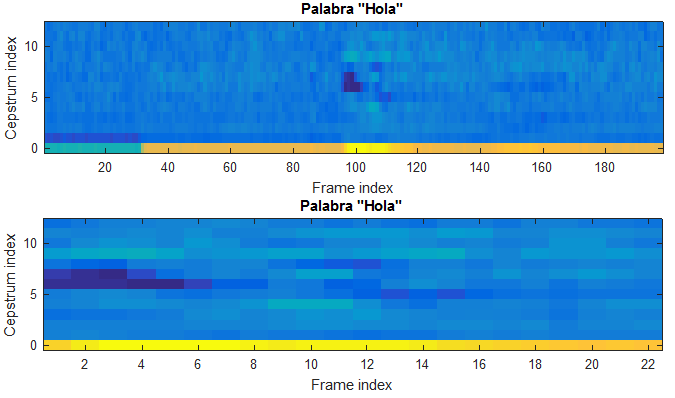
\includegraphics[width=0.8\linewidth]{figures/mfccHolaRecorte}
			\caption{Coeficientes en la escala de Mel, palabra ``Hola''.}
			\label{fig:ana:HolaRecorte}
	\end{figure}
	
	En la Figuras \ref{fig:ana:mfccHola} y \ref{fig:ana:mfccTren} se muestran los coeficientes cepstrales en la escala de Mel de las palabras \textit{Hola} y \textit{Tren} pronunciadas por diferentes personas. Como se puede observar, entre los coeficientes de la misma palabra existen ciertas similitudes como la intensidad en los segmentos, mientras que entre los diferentes interlocutores se observan ciertas características, por ejemplo, en los primeros segmentos en el coeficiente 5 se observa menor intensidad que para el hombre en los mismos coeficientes, esto puede dar pie a reconocer el sexo del interlocutor o inclusive al interlocutor.
	
	 \begin{figure}[H]
			\centering
			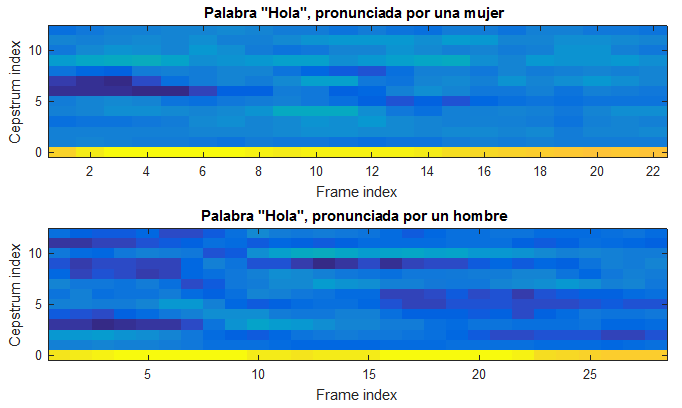
\includegraphics[width=0.8\linewidth]{figures/mfccHola}
			\caption{Palabra ``Hola' pronunciada por diferentes personas'.}
			\label{fig:ana:mfccHola}
	\end{figure}
	
	 \begin{figure}[H]
			\centering
			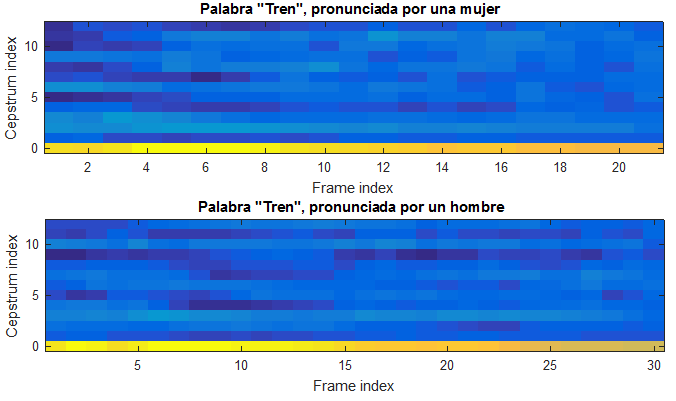
\includegraphics[width=0.8\linewidth]{figures/mfccTren}
			\caption{Palabra ``Tren'' pronunciada por diferentes personas.}
			\label{fig:ana:mfccTren}
	\end{figure}
	
	Y como complemento se propone el uso de cuantización vectorial debido al alto desempeño mostrado en \cite{A6}, \cite{A7} y \cite{A8}, además de que surge la necesidad de tener un tamaño fijo en los vectores de características ya que éstos serviran de entrada a la red neuronal que llevará a cabo el reconocimiento de las palabras, como se ve en las Figuras \ref{fig:ana:HolaRecorte}, \ref{fig:ana:mfccHola} y \ref{fig:ana:mfccTren} el índice se segmento varía, por lo que el número de coeficientes total depende de la duración de la muestra de voz.
	
	Finalmente, se opta por el uso de las redes neuronales, de acuerdo a los resultados obtenidos de \cite{A3} se propone el uso de una red neuronal \textit{feedforward} en su versión de \textit{Pattern Recognition Network} y para el entrenamiento se propone el uso del algoritmo \textit{Scaled Conjugate Gradient backpropagation} debido al alto desempeño que muestran en conjunto para reconocimiento de voz en señales con baja relación señal a ruido.

\subsection{Propuesta de frases}

Como propuesta inicial se plantea la obtención de las frases a reconocer de tres categorías de frases que corresponden a saludos, compras y la ciudad.

\paragraph{Saludos}\paragraph{}

Dentro de la costumbre mexicana, el saludo es un punto que hay que tener en cuenta, así como también los modales, es por eso que dentro de esta categoría se plantea el siguiente diccionario de palabras con las cuales se pueden formar diversos saludos y respuestas a éstos.

\begin{itemize}
\item	Buenos/Buenas: Se coloca una letra b sobre el corazón, y se mueve al frente.
\item	Hola: Se coloca una letra h sobre la frente, y se mueve hacia arriba.
\item	Días: se hace una d, y se mueve en medio círculo hacia un lado.
\item	Tardes: se coloca una t sobre el antebrazo, y se mueve en línea recta hacia usted.
\item	Noches: se coloca una g sobre la frente, y se mueve hacia abajo.
\end{itemize}

Así, de esta forma se cubren las frases básicas para esta categoría son:

 
\begin{table}[H]
\centering
\caption{Frases seleccionadas para la sección de saludos}
\label{tb:saludosFrases}
\begin{tabular}{|c|c|}
\hline
Hola, ¡buenos días!   & Hola, ¡buenas noches! \\ \hline
Hola, ¡buenas tardes! &                       \\ \hline
\end{tabular}
\end{table}
 
\paragraph{Compras}\paragraph{}

Uno de los aspectos cotidianos es el ir de compras, ya sea a la tienda o un súper mercado, esta categoría es extensa pues se pueden abordar diferentes tipos de compras, sin embargo, se tratará de una selección de frases que puedan ser usadas en cualquier sitio de compra. Estas frases fueron seleccionadas de una guía de frases en inglés haciendo referencia a compras. 

\begin{table}[H]
\centering
\caption{Frases seleccionadas para la sección de compras}
\label{tb:comprasFrases}
\begin{tabular}{|l|l|}
\hline
¿A qué hora abren?          & ¿Cuánto cuesta?          \\ \hline
¿A qué hora cierran?        & Estoy buscando (objeto), \\ \hline
¿Acepta tarjeta de crédito? & Me llevo esto.           \\ \hline
\end{tabular}
\end{table}
 
De este conjunto de frases se obtienen nuevas palabras que se reconocerán en el sistema

\paragraph{Ciudad}\paragraph{}

La tercera categoría abarca frases relacionadas con la ciudad, la utilidad de esta sección es para pedir informes dentro de la ciudad, así como también pedir indicaciones. Al igual que la categoría anterior, estas frases fueron seleccionadas de la misma guía anteriormente mencionada. 

\begin{table}[H]
\centering
\caption{Frases seleccionadas para la sección de ciudad}
\label{tb:ciudadFrases}
\begin{tabular}{|l|l|}
\hline
¿Disculpe, dónde está …?  & ¿Hay algún … cerca? \\ \hline
La oficina de información & Cajero              \\ \hline
La estación de autobuses  & Banco               \\ \hline
La estación de trenes     & Supermercado        \\ \hline
La estación de policía    & Farmacia            \\ \hline
                          & Metro               \\ \hline
                          & Hospital            \\ \hline
                          & Biblioteca          \\ \hline
\end{tabular}
\end{table}
 
Ya seleccionadas las frases con las que se trabajarán en la tabla 1 se presenta el listado general de palabras a reconocer.

\begin{table}[H]
\centering
\caption{Listado de palabras}
\label{tb:listadoPalabras}
\begin{tabular}{|l|l|l|}
\hline
\multicolumn{3}{|l|}{Listado de palabras por categoría} \\ \hline
Hola               & Estoy           & Estación         \\ \hline
Buenos/Buenas      & Buscando        & Autobuses        \\ \hline
Días               & Cuánto          & Trenes           \\ \hline
Tardes             & Cuesta          & Policía          \\ \hline
Noches             & Me              & Hay              \\ \hline
A                  & Llevo           & Algún            \\ \hline
Qué                & Esto            & Cerca            \\ \hline
Hora               & Disculpe        & Cajero           \\ \hline
Abren              & Dónde           & Banco            \\ \hline
Cierran            & Está            & Supermercado     \\ \hline
Acepta             & La              & Farmacia         \\ \hline
Tarjeta            & Oficina         & Metro            \\ \hline
De                 & Hospital        & Crédito          \\ \hline
Información        & Biblioteca      &                  \\ \hline
\end{tabular}
\end{table}


\subsection{Especificación de requisitos de software}

En esta sección se presenta la Especificación de Requisitos de Software (ERS) para la aplicación móvil que forma parte del proyecto terminal “Aplicación móvil para la comunicación con personas que utilizan el Lenguaje de Señas Mexicano (LSM)” según el estándar de IEEE 830.

%\subsubsection{Propósito}

%El propósito de este documento es definir la estructura y diseño de la aplicación móvil. Este documento va dirigido a toda persona interesada en el funcionamiento y estructuración del software a desarrollar.

\subsubsection{Ámbito del software}

\begin{itemize}
\item	La aplicación móvil llevará por nombre “Voice hands”.
\item	La aplicación interpretará un mensaje de voz a lenguaje de señas, representando el mensaje por medio de imágenes o animaciones.
\item	La aplicación no guardará los mensajes de voz.
\item	La aplicación contará con la capacidad de realizar síntesis de voz.
\item	No se podrán enviar mensajes digitales a través de la aplicación con otros usuarios.
\item	La aplicación permite la consulta de un diccionario del LSM por categorías.
\item	La aplicación reconocerá e interpretará cierta cantidad de frases limitadas por 43 palabras que se encuentran en el banco de reconocimiento.
\item	Con el desarrollo de esta aplicación se espera que las personas que utilizan el lenguaje de señas sean capaces de comunicarse con personas que no y a su vez, las personas que no hacen uso de éste sean capaces de comunicarse con personas que sí.
\item	Un beneficio de esta aplicación es que cualquier persona que cuente con un móvil Android podrá hacer uso de ella, sin hardware adicional.
\item	El objetivo de la aplicación móvil es lograr que las personas tengan mayor oportunidad de acercamiento a tecnologías que permitan realizar la comunicación sin hacer uso de hardware adicional.
\item	Se espera que el software en un futuro pueda ser capaz de admitir una ampliación a su vocabulario a reconocer.
\end{itemize}

\subsubsection{Del sistema}

\begin{itemize}
\item	La aplicación móvil tendrá conexión al servidor que llevará a cabo el procesamiento de voz y nos entregará el resultado, la conexión mediante Internet.
\item	El sistema permitirá el uso en cualquier momento.
\item	El sistema soportará diversas peticiones al mismo tiempo, el número de peticiones está por definirse de acuerdo a los algoritmos implementados.
\end{itemize}

\subsubsection{Visión general}

En las secciones siguientes se detalla la estructura y funcionamiento de la aplicación móvil, los requisitos del dispositivo que la ejecutará, diagramas de casos de uso, actividades y un esbozo general de la aplicación.

\subsubsection{Descripción general}
\paragraph{Perspectiva del producto}\paragraph{}

La aplicación móvil será totalmente independiente a cualquier otro producto, en un futuro la unión de dos aplicaciones no queda descartada, pues existen productos desarrollados y en desarrollo que contribuyen al proceso de comunicación con el uso del LSM y esta unión se podrá dar gracias a un content provider entre ambas aplicaciones. Para este trabajo se desarrollará la aplicación móvil que realice la traducción de un mensaje de voz a lenguaje de señas, se diseñará la aplicación móvil y desarrollará el sistema que permita el procesamiento de voz.

\paragraph{Funciones del producto}\paragraph{}

La aplicación móvil contará con tres funciones principales:

\begin{itemize}
\item	Traducción de voz a LSM: Esta función básicamente graba una frase en voz y la traduce a lenguaje de señas mexicana, mostrando el resultado mediante imágenes.
\item	Reproducción en voz de cualquier texto ingresado: Se toma el texto ingresado en un campo de texto y se realiza la síntesis en voz de éste.
\item	Consulta de un diccionario de LSM: Organizado por categorías, se podrán consultar palabras del LSM y la forma en que se realizan dichas señas.
\end{itemize}

\paragraph{Características de los usuarios}\paragraph{}

La aplicación móvil va dirigida a personas con interés de comunicarse principalmente con personas sordas que utilizan el LSM, además, también va dirigido a personas que utilizan el lenguaje de señas y que tienen interés en comunicarse con personas que no lo usan, estas personas deberán tener conocimiento básico del uso de aplicaciones móviles.

\paragraph{Restricciones y limitaciones}

El uso de esta aplicación se recomienda en dispositivos móviles con las siguientes características mínimas:
\begin{itemize}
\item	Smartphone Android versión 4.4.
\item	Memoria RAM de 1 GB.
\item	Memoria interna de 8 GB con memoria externa.
\item	CPU: Quad-core 1.4 GHz
\end{itemize}

Para el servidor que realizará el procesamiento:
\begin{itemize}
\item	Windows 8 o superior.
\item	Java 8 o superior.
\item	4 GB de memoria RAM.
\item	10 GB de disco duro disponibles.
\item	Procesador de doble núcleo a 1.8 GHz.
\item	MySQL server 5.6.
\end{itemize}

La aplicación será desarrollada en Android Studio versión 2.2 bajo el lenguaje de programación Java, el procesamiento de voz se llevará a cabo en un servidor con lenguaje C.

La comunicación con el servidor se llevará a cabo mediante web service a través del protocolo TCP/IP.

La aplicación móvil no contará con sistema de seguridad ya que no se estarán manejando datos delicados ni registro en ésta.

\paragraph{Suposiciones y dependencias}\paragraph{}

La aplicación móvil está diseñada para Android, si se desea migrar a otro sistema operativo se deberán revisar los requisitos del dispositivo, así como el cambio de desempeño e interfaces con el servidor, de igual forma, si el servidor se implementa en un sistema operativo, será necesario revisar la comunicación que se llevará a cabo con la aplicación móvil.

El número de palabras y/o frases en un futuro puede crecer, así que es posible que se requiera un servidor con mayor capacidad de procesamiento para llevar a cabo el reconocimiento de palabras.

\paragraph{Requisitos futuros}\paragraph{}

Las posibles mejoras a la aplicación serían la integración de un diccionario más amplio de reconocimiento, integración de un sistema de reconocimiento de imágenes para completar la comunicación bidireccional e incluir un curso sobre lenguaje de señas.

\subsubsection{Requisitos específicos}

\paragraph{Interfaces externas}

\begin{itemize}
\item	Ie1. La aplicación móvil tendrá una interfaz sencilla que permita al usuario intuir el funcionamiento y la sección de funciones de ésta.
\item	Ie2. La comunicación con el servidor se llevará a cabo mediante un web service a través del protocolo TCP-IP.
\item	Ie3. Para la realización de la función de \textit{text-to-speech} o síntesis de voz se hará uso de la API que Google nos proporciona.
\item	Ie4. El servidor utilizará el ODBC más adecuado  para comunicarse con la base de datos.
\end{itemize}

\paragraph{Funciones}
\begin{enumerate}[label=(\alph*)]
\item	Traductor de voz a LSM

\begin{itemize}
\item	Fa1. Se contará con un botón para iniciar la grabación de la voz. (Móvil)
\item	Fa2. Se enviará la voz o las características de ésta al servidor a través de un web service. (Móvil)
\item	Fa3. Se realizará el procesamiento de voz para determinar las palabras mencionadas. (Servidor)
\item	Fa4. Se mapeará la frase detectada con la estructura correspondiente al LSM. (Servidor)
\item	Fa5. Se leerá de la base de datos las imágenes o animaciones correspondientes a la frase detectada. (Servidor)
\item	Fa6. Se enviará a la aplicación móvil las imágenes o códigos de éstas para que en la pantalla muestre el mensaje con la estructura correcta. (Servidor)
\item	Fa7. La aplicación móvil mostrará en pantalla las imágenes o animaciones correspondientes a la frase mencionada.
\item	Fa8. El usuario sólo podrá decir frases cortas con duración no mayor a 10 segundos.
\end{itemize}

\item	Síntesis de voz a través del teclado

\begin{itemize}
\item	Fb1. El usuario a través del teclado en pantalla ingresa la frase a comunicar.
\item	Fb2. Haciendo uso de la API de Google de text to speech se realizará la síntesis del texto introducido.
\item	Fb3. El idioma soportado será el español de México.
\end{itemize}

\item	Diccionario del LSM

\begin{itemize}
\item	Fc1. El diccionario estará dividido por categorías.
\item	Fc2. Contará con filtros por categoría y un cuadro de búsqueda.
\item	Fc3. Al seleccionar la palabra, la aplicación le mostrará la imagen correspondiente, además de una breve descripción de su uso.
\end{itemize}

\end{enumerate}

Estas secciones serán alcanzables gracias a un menú lateral que nos ofrecerá la opción de ingresar a cada una.

\paragraph{Requisitos de rendimiento}
\begin{itemize}
\item	Rr1. La aplicación sólo podrá ejecutar una actividad a la vez, y será usada por un usuario.
\item	Rr2. La aplicación se conectará con el servidor que ejecutará el procesamiento de la voz.
\item	Rr3. El servidor tendrá la capacidad de atender a más de un usuario a la vez .
\item	Rr4. Se requiere que la aplicación cuente con conexión a Internet.
\item	Rr5. Dado el listado de palabras se plantea que la cantidad de registros almacenados en la base de datos sea en el orden de las decenas.
\end{itemize}

\paragraph{Restricciones de diseño}
\begin{itemize}
\item	Rd1. La interfaz de la aplicación móvil se desarrollará en Android Studio, haciendo uso de las formas ya establecidas.
\item	Rd2. La interfaz gráfica de la aplicación móvil se llevará a cabo siguiendo el diseño visual y de movimientos de la guía de Material Design para Android.
\item	Rd3. La interfaz será de fácil entendimiento para que todas las personas que lo deseen la puedan ocupar.
\item	Rd4. El servidor no contará con interfaz gráfica.
\item	Rd5. Se hará uso del diccionario “manos con voz” de María Serafín y Raúl González para la obtención de imágenes.
\end{itemize}

\paragraph{Atributos de la aplicación}
\begin{itemize}
\item	Aa1. La aplicación será diseñada para que pueda ser usada por todo tipo de personas.
\item	Aa2. No se requiere de un inicio de sesión, por lo que en un móvil pueden interactuar más personas.
\item	Aa3. Como trabajo a futuro serán ofrecidas las actualizaciones que permitan más características, así como también nuevas funciones.
\end{itemize}


\section{Diseño}

En esta sección se muestra el diseño del sistema que será implementado, los diagramas de los procesos que se llevarán a cabo, los diagrmas de actividades y UML,esta sección se divide en dos secciones, el diseño del reconocimiento de voz y el diseño de la aplicación.

\subsection{Diseño del reconocimiento de voz}

De acuerdo a lo visto en la sección de análisis en la Figura \ref{fig:SRgeneral} se muestra el diagrama general del reconocimiento de voz que será implementado para llevar a cabo el reconocimiento de las palabras a ser traducidas al lenguaje de señas.

		\begin{figure}[H]
			\centering
			
\includegraphics[width=1\linewidth]{figures/srGeneral}
			\caption{Diagrama general del reconocimiento de voz.}
			\label{fig:SRgeneral}
		\end{figure}
		
\subsubsection*{Pre-procesamiento}		

El pre-procesamiento de la señal de voz se llevará a cabo de acuerdo al diagrama de la  Figura \ref{fig:preprocesamientoDes}, esta étapa consta de cuatro bloques que se explican a continucación.

		\begin{figure}[H]
			\centering
			\includegraphics[width=1\linewidth]{figures/preprocesamientoDes}
			\caption{Diagrama de la etapa de pre-procesamiento.}
			\label{fig:preprocesamientoDes}
		\end{figure}
		
	\begin{itemize}
		\item	\textbf{Detección de bordes y separación de palabras:} esta etapa llevará a cabo la detección de bordes de las palabras invlucradas en la oración (señal de voz a reconocer) ya que se tratarán con frases y el número de palabras puede variar. De acuerdo a la sección del análisis, se hará uso del algoritmo que aprovecha las características de energía de señal y tasa de cruces por cero del dominio del tiempo y el centroide y flujo espectral del dominio frecuencial propuesto en \cite{A31}, una vez segmentada la frase en palabras, cada señal de voz correspondiente a una palabra será procesada de forma individual.
		\item	\textbf{Filtro preénfasis:} el filtro aplicado será un filtro digital de primer orden y de acuerdo al análisis el coeficiente $a$ de la ecuación $\hat{s}(n)=s(n)-a\cdot s(n-1)$ será igual a $0.95$.
		\item	\textbf{Segmentación:} la segmentación de la señal de voz se realizará con una duración de 40 ms del segmento y un traslape de 20 ms.
		\item	\textbf{Aplicación de ventana:} finalmente se aplicará la ventana de Hamming de acuerdo al análisis hecho en la sección anterior.
	\end{itemize}
	
	\subsubsection*{Extracción de características}
	
	La señal resultante del pre-procesamiento sirve de entrada al bloque de extracción de características, para la extracción de características se ha decidido realizar por medio de los MFCC que se realiza de acuerdo a la Figura \ref{fig:extraccionMFCC}.
	
		\begin{figure}[H]
			\centering
			\includegraphics[width=1\linewidth]{figures/extraccionMFCC}
			\caption{Cálculo de los coeficientes MFCC.}
			\label{fig:extraccionMFCC}
		\end{figure}

	\subsubsection*{Red neuronal}
		
	La red neuronal que se implementará para llevar a cabo el reconocimiento de patrones será una arquitectura \textit{feedforward Pattern Recognition} y será entrenada con el algoritmo de entrenamiento \textit{Scaled Conjugate Gradient backpropagation} y como función de activación para la capa oculta se usará \textit{sigmoid} y en la capa de salida \textit{softmax}. Los vectores de entrada a la red serán los vectores de coeficientes cepstrales cuantizados vectorialmente, de esta forma se asegura una longitud fija de los vectores.

\subsection{Diseño de la aplicación}

En esta sección se muestra el diseño de la aplicación móvil mediante diagramas y el boceto de ésta. Los diagramas que se presentan son de casos de uso, de actividades, diseño de la base de datos y finalmente las pantallas de la aplicación, de esta forma se tendrá un mayor entendimiento de la secuencia de la aplicación y su estructuración.

\subsubsection{Diagrama de casos de uso}

Los siguientes diagramas junto con sus tablas muestran los casos de uso de la aplicación, así como los factores que intervienen.

En la Figura \ref{fig:casoUsoGen} se muestra un diagrama general de la aplicación mostrando el uso que puede hacer el usuario de la aplicación, en este caso son tres actividades principales: 

\begin{itemize}
\item	Traductor de voz a LSM.
\item	Síntesis de voz desde el teclado.
\item	Consulta de diccionario.
\end{itemize}

		\begin{figure}[H]
			\centering
			\includegraphics[width=0.8\linewidth]{figures/casoUsoGeneral}
			\caption{Caso de uso general}
			\label{fig:casoUsoGen}
		\end{figure}	
		
Como observamos, se cuenta con un tipo de usuario y del otro lado la opción del traductor hace uso del servidor para enviar y recibir información respecto a la frase grabada.

\paragraph{Traductor de voz a LSM}\paragraph{}

En la Tabla \ref{tb:casoUsoVoz} se muestra la especificación de la Figura \ref{fig:casoUsoVoz} correspondiente al caso de uso de traductor de voz a LSM, en este caso tenemos a un usuario que desea comunicarse con una persona que usa el LSM.		

\begin{table}[H]
\centering
\caption{Caso de uso \textit{``Traductor de voz''}}
\label{tb:casoUsoVoz}
\begin{tabular}{|l|l|}
\hline
\multicolumn{2}{|l|}{\cellcolor[HTML]{C0C0C0}Caso de uso: Traductor de voz a LSM}                                                                                                                                                                                                             \\ \hline
\multicolumn{2}{|l|}{Actor: Usuario, Aplicación móvil y Servidor}                                                                                                                                                                                                                             \\ \hline
\multicolumn{2}{|l|}{Descripción: Permite realizar la traducción del mensaje de voz grabado a LSM}                                                                                                                                                                                            \\ \hline
Curso normal                                                                                                                                            & Alternativas                                                                                                                        \\ \hline
\begin{tabular}[c]{@{}l@{}}1.	El usuario selecciona la función de \\ traductor\end{tabular}                                                             &                                                                                                                                     \\ \hline
\begin{tabular}[c]{@{}l@{}}2.	Deja presionado el botón de grabar \\ y se guarda el mensaje.\end{tabular}                                                &                                                                                                                                     \\ \hline
\begin{tabular}[c]{@{}l@{}}3.	Al terminar la grabación se envía al \\ servidor para su debido procesamiento.\end{tabular}                               & \begin{tabular}[c]{@{}l@{}}3.1.,Si no está disponible el servidor, se le \\ hará saber al usuario.\end{tabular}                     \\ \hline
\begin{tabular}[c]{@{}l@{}}4.	El servidor busca la palabra detectada \\ en la base de datos.\end{tabular}                                               & \begin{tabular}[c]{@{}l@{}}4.1.,Si no reconoce la palabra o no está en la \\ base de datos se le informará al usuario.\end{tabular} \\ \hline
\begin{tabular}[c]{@{}l@{}}5.	Se envía el resultado a la aplicación \\ móvil.\end{tabular}                                                              &                                                                                                                                     \\ \hline
\begin{tabular}[c]{@{}l@{}}6.	Se muestra en pantalla el resultado de \\ la traducción, así como también los \\ posibles mensajes de error.\end{tabular} &                                                                                                                                     \\ \hline
\end{tabular}
\end{table}

		\begin{figure}[H]
			\centering
			\includegraphics[width=0.8\linewidth]{figures/casoUsoVoz}
			\caption{Caso de uso \textit{``Traductor de voz''}}
			\label{fig:casoUsoVoz}
		\end{figure}
		
\paragraph{Síntesis de voz desde el teclado}\paragraph{}

En la Tabla \ref{tb:casoUsoSintesis} se muestra la especificación de la Figura \ref{fig:casoUsoSintesis} que corresponde al caso de uso de síntesis de voz en el cual, la persona que usa el LSM desea comunicarse con una persona que no lo usa.
		
\begin{table}[H]
\centering
\caption{Caso de uso \textit{``Síntesis de voz desde el teclado''}}
\label{tb:casoUsoSintesis}
\begin{tabular}{|l|l|}
\hline
\multicolumn{2}{|l|}{\cellcolor[HTML]{C0C0C0}Caso de uso: Síntesis de voz desde el teclado}                                                                                                                              \\ \hline
\multicolumn{2}{|l|}{Actor: Usuario, Aplicación móvil}                                                                                                                                                                   \\ \hline
\multicolumn{2}{|l|}{Descripción: Permite llevar a cabo la síntesis de voz del texto ingresado mediante el teclado}                                                                                                      \\ \hline
Curso normal                                                                                          & Alternativas                                                                                                     \\ \hline
\begin{tabular}[c]{@{}l@{}}1.	El usuario selecciona la función de \\ síntesis de voz\end{tabular}     &                                                                                                                  \\ \hline
\begin{tabular}[c]{@{}l@{}}2.	El usuario ingresa el texto en un campo \\ destinado.\end{tabular}      &                                                                                                                  \\ \hline
\begin{tabular}[c]{@{}l@{}}3.	Se da la opción de reproducir para \\ escuchar el mensaje.\end{tabular} & \begin{tabular}[c]{@{}l@{}}3.1.,Si el dispositivo no tiene conexión a \\ Internet se la hará saber.\end{tabular} \\ \hline
4.	Se reproduce el mensaje.                                                                           &                                                                                                                  \\ \hline
\end{tabular}
\end{table}

		\begin{figure}[H]
			\centering
			\includegraphics[width=0.8\linewidth]{figures/casoUsoSintesis}
			\caption{Caso de uso \textit{``Síntesis de voz desde el teclado''}}
			\label{fig:casoUsoSintesis}
		\end{figure}
		
\paragraph{Consulta de diccionario}\paragraph{}

En la Tabla \ref{tb:casoUsoDicc} se muestra la especificación de la Figura \ref{fig:casoUsoDicc} que corresponde al caso de uso de consulta de diccionario, en el que podemos encontrar vocabulario de diferentes categorías, así como las instrucciones para llevar a cabo la seña correspondiente.

% Please add the following required packages to your document preamble:
% \usepackage[table,xcdraw]{xcolor}
% If you use beamer only pass "xcolor=table" option, i.e. \documentclass[xcolor=table]{beamer}
\begin{table}[H]
\centering
\caption{Caso de uso \textit{``Consulta de diccionario''}}
\label{tb:casoUsoDicc}
\scalebox{0.9}{
\begin{tabular}{|l|l|}
\hline
\multicolumn{2}{|l|}{\cellcolor[HTML]{C0C0C0}Caso de uso: Consulta de diccionario}                                                                                                                                                           \\ \hline
\multicolumn{2}{|l|}{Actor: Usuario, Aplicación móvil, base de datos local.}                                                                                                                                                                 \\ \hline
\multicolumn{2}{|l|}{\begin{tabular}[c]{@{}l@{}}Descripción: Permite realizar la consulta de una palabra \\ obteniendo la seña e instrucciones para llevarla a cabo.\end{tabular}}                                                           \\ \hline
Curso normal                                                                                                 & Alternativas                                                                                                                  \\ \hline
\begin{tabular}[c]{@{}l@{}}1.   El usuario selecciona la función de consulta de\\  diccionario.\end{tabular} &                                                                                                                               \\ \hline
2.   Selecciona la categoría a consultar.                                                                    &                                                                                                                               \\ \hline
3.   Selecciona la palabra deseada.                                                                          & \begin{tabular}[c]{@{}l@{}}3.1.   Puede hacer uso del filtro de palabras\\ para encontrar más rápido la deseada.\end{tabular} \\ \hline
4.   Se muestra la información en pantalla.                                                                  &                                                                                                                               \\ \hline
\end{tabular}}
\end{table}

		\begin{figure}[H]
			\centering
			\includegraphics[width=0.8\linewidth]{figures/casoUsoDicc}
			\caption{Caso de uso \textit{``Consulta de diccionario''}}
			\label{fig:casoUsoDicc}
		\end{figure}
		
\subsubsection{Diagramas de actividades}

En la Figura \ref{fig:actVoz} se muestra la actividad del traductor de voz, así como las acciones que se deben llevar a cabo tanto por el usuario como por el móvil para obtener la traducción.


		\begin{figure}[H]
			\centering
			\includegraphics[width=0.5\linewidth]{figures/actVoz}
			\caption{Diagrama de actividad \textit{``Traductor de voz a LSM''}}
			\label{fig:actVoz}
		\end{figure}
		
En la Figura \ref{fig:actSintesis} se muestra el proceso a seguir para llevar a cabo la síntesis de voz mediante la entrada de texto

		\begin{figure}[H]
			\centering
			\includegraphics[width=0.2\linewidth]{figures/actSintesis}
			\caption{Diagrama de actividad \textit{``Síntesis de voz desde teclado''}}
			\label{fig:actSintesis}
		\end{figure}
		
En la Figura \ref{fig:actDicc} se muestra la acción de consultar el diccionario y el flujo de la consulta dependiendo de si se usa o no los filtros disponibles.		

		\begin{figure}[H]
			\centering
			\includegraphics[width=0.5\linewidth]{figures/actDicc}
			\caption{Diagrama de actividad \textit{``Consulta de diccionario''}}
			\label{fig:actDicc}
		\end{figure}
		
\subsubsection{Diagramas de secuencia}

En los siguientes diagramas se muestra la secuencia de actividades a llevar a cabo para realizar las 3 tareas planteadas.

En la Figura \ref{fig:secVoz} se muestra la secuencia y la intervención de cada elemento del sistema para llevar a cabo la adquisición de voz y su respectiva traducción.

		\begin{figure}[H]
			\centering
			\includegraphics[width=0.7\linewidth]{figures/secuenciaVoz}
			\caption{Diagrama de secuencia \textit{``Traductor de voz a LSM''}}
			\label{fig:secVoz}
		\end{figure}
		
En la Figura \ref{fig:secSintesis} se muestra el diagrama de secuencia que muestra la interacción entre el actor y el dispositivo móvil para llevar a cabo la síntesis de voz del mensaje a transmitir.

		\begin{figure}[H]
			\centering
			\includegraphics[width=0.5\linewidth]{figures/secuenciaSintesis}
			\caption{Diagrama de secuencia \textit{``Síntesis de voz desde teclado''}}
			\label{fig:secSintesis}
		\end{figure}		
		
Finalmente en la Figura \ref{fig:secDiccionario} se muestra la interacción entre el actor y el dispositivo móvil, con las acciones a realizar para obtener la descripción de la seña de determinada palabra.

		\begin{figure}[H]
			\centering
			\includegraphics[width=0.5\linewidth]{figures/secuenciaDiccionario}
			\caption{Diagrama de secuencia \textit{``Consulta de diccionario''}}
			\label{fig:secDiccionario}
		\end{figure}		
		
\subsubsection{Base de datos}

La base de datos a implementar básicamente será una tabla la cual contendrá la palabra un código asociado, este código identificará a la imagen que debe ser presentada, el código será enviado al móvil el cual ya contiene todas las imágenes que corresponden a las palabras. En la Figura \ref{fig:database} se muestra la tabla de la base de datos a implementar.

		\begin{figure}[H]
			\centering
			\includegraphics[width=0.5\linewidth]{figures/database}
			\caption{Base de datos a implementar}
			\label{fig:database}
		\end{figure}		

\subsubsection{Pantallas de la aplicación}

%\begin{multicols}{2} 

\begin{figure}[H]
	\centering
	\includegraphics[scale = 0.2]{figures/app01}
	\caption{Aplicación: Splash Screen}
	\label{fig:app01}
\end{figure}

La primera pantalla de la aplicación es un Splash Screen en la cual se muestra en nombre e icono durante 3 segundos.

\begin{figure}[H]
	\centering
	\includegraphics[scale = 0.2]{figures/app02}
	\caption{Aplicación: Menú lateral}
	\label{fig:app03}
\end{figure}

La aplicación cuenta con un menú lateral que nos mostrará las tres principales actividades, y mediante las cuales podremos acceder.

\begin{figure}[H]
	\centering
	\includegraphics[scale = 0.2]{figures/app03}
	\caption{Aplicación: Pantalla principal}
	\label{fig:app02}
\end{figure}

La pantalla principal corresponde a la sección de traductor de voz a LSM.

\begin{figure}[H]
	\centering
	\includegraphics[scale = 0.2]{figures/app04}
	\caption{Aplicación: Grabación de voz}
	\label{fig:app04}
\end{figure}

Al seleccionar el traductor de voz a LSM contaremos con un botón flotante que es el que nos permitirá grabar la frase que queremos traducir, y se nos mostrará una barra de progreso lo que nos indica el tiempo restante para completar la grabación.

\begin{figure}[H]
	\centering
	\includegraphics[scale = 0.2]{figures/app05}
	\caption{Aplicación: Traducción}
	\label{fig:app05}
\end{figure}

Una vez hecho esto, el sistema se encarga de enviar y recibir la información, para que después nos muestre en pantalla la imagen o imágenes resultantes de la traducción.

\begin{figure}[H]
	\centering
	\includegraphics[scale = 0.2]{figures/app06}
	\caption{Aplicación: Campo de escritura para síntesis}
	\label{fig:app06}
\end{figure}

Si seleccionamos la segunda opción del menú lateral o la síntesis de voz, la aplicación nos mostrará esta actividad, en la cual tan sólo debemos ingresar el texto en el cuadro y al finalizar presionamos el botón pronunciar para que se realice la síntesis de voz.

\begin{figure}[H]
	\centering
	\includegraphics[scale = 0.2]{figures/app07}
	\caption{Aplicación: Entrada de texto}
	\label{fig:app07}
\end{figure}

En esta pantalla vemos cómo se muestra el teclado y se realiza la entrada de texto.

\begin{figure}[H]
	\centering
	\includegraphics[scale = 0.2]{figures/app08}
	\caption{Aplicación: Reproducción de voz}
	\label{fig:app08}
\end{figure}

Finalmente se presiona el botón y a través de los altavoces se escuchará la frase.

\begin{figure}[H]
	\centering
	\includegraphics[scale = 0.2]{figures/app09}
	\caption{Aplicación: Categorías del diccionario}
	\label{fig:app09}
\end{figure}

Finalmente, si seleccionamos la tercera opción o el diccionario veremos esta actividad, la cual nos muestra el diccionario dividido en categorías.

\begin{figure}[H]
	\centering
	\includegraphics[scale = 0.2]{figures/app10}
	\caption{Aplicación: Palabras de una categoría}
	\label{fig:app10}
\end{figure}

Una vez seleccionada la categoría podremos seleccionar la palabra buscada o en el cuadro de texto podemos filtrar las palabras de acuerdo a lo que buscamos.

\begin{figure}[H]
	\centering
	\includegraphics[scale = 0.2]{figures/app11}
	\caption{Aplicación: Información de la palabra}
	\label{fig:app11}
\end{figure}

Una vez seleccionada la palabra, la aplicación nos mostrará otra actividad con la información relacionada a ésta, tanto la seña en imagen y la instrucción para realizarla, también en algunos casos se encontrará información adicional.

%\end{multicols}

\section{Conclusiones}

Durante el desarrollo de Proyecto Terminal I se lograron definir las técnicas y herramientas a usar para el desarrollo del sistema propuesto que surge de la falta de inclusión de personas que tienen problemas de audición a las actividades diarias que se desempeñan en la ciudad, para esto se propuso una aplicación móvil que permite llevar a cabo la comunicación entre personas que utilizan el lenguaje de señas con personas que no lo usan a través de un sistema de reconocimiento de voz que traduce las palabras habladas a imágenes del lenguaje de señas mexicano que corresponden a estas palabras.

En cuanto al reconocimiento de voz se determinaron las técnicas que se llevaran a cabo para cumplir con esta tarea, para el pre-procesamiento se definieron las características para la obtención de la señal de voz las cuales son una frecuencia d muestreo de 8 kHz y un PCM de 8 bits debido a que se requieren tiempos de procesamiento no mayores a 5 segundos para mantener la conversación fluida, se estableció el uso de un filtro preénfasis para resaltar las características frecuenciales de la señal de voz y se determinó el uso de la energía de la señal y tasa de cruces por cero (características de la señal en el dominio del tiempo) para llevar a cabo la detección de bordes de la señal y así eliminar los silencios. Se determinó el uso de la técnica de extracción de características MFCC debido a los buenos resultados obtenidos en los trabajos presentados en el estado del arte y finalmente se empleará la cuantización vectorial a los coeficientes obtenidos de la extracción de características, así se tendrá una longitud fija en el vector de características que servirá de entrada a la red neuronal.

De acuerdo a los trabajos analizados se determinó el uso de la arquitectura \textit{feedforward Pattern Recognition} y el algoritmo de entrenamiento \textit{Scaled Conjugate Gradient backpropagation} a emplear en la red neuronal que realizará el reconocimiento de patrones de los vectores de características y de esta forma determinar las palabras que corresponden a la señal de voz, como funciones de activación se emplearan \textit{sigmoid} para la capa oculta y \textit{softmax} para la capa de salida.

El diseño de la aplicación se basó en un análisis de requerimientos con la norma IEEE 830, obteniendo el diseño de las pantallas de la aplicación móvil que se resumen en tres secciones: el reconocimiento de palabras, síntesis de voz y diccionario, el lenguaje de programación a emplear para llevar a cabo el reconocimiento es C debido al manejo más eficiente que se logra a comparación de otros lenguajes y el \textit{Web Service} se implementará en Java, el desarrollo de la aplicación móvil se llevará a cabo en \textit{Android Studio}.

Se logró definir el banco de palabras propuesto a reconocer que consta de un total de 42 palabras que corresponden a tres categorías de la comunicación básica para saludar, pedir indicaciones y solicitar ayuda.

Se logró implementar en la aplicación móvil la síntesis de mensajes escritos a voz con ayuda de la API de Google y el diccionario auxiliar que contiene seis categorías y en cada categoría se encuentra la descripción de la seña que corresponden a las palabras.

En esta primera parte se logró definir la arquitectura, técnicas y métodos a emplear para llevar a cabo el reconocimiento de voz y la implementación del sistema. Con el diseño propuesto se pueden llevar a cabo las actividades propuestas en el cronograma de Proyecto Terminal II para llevar a cabo la implementación del sistema y sus respectivas pruebas.


\section{Lista de acrónimos}

\begin{itemize}

\item	LSM - Lengua de Señas Mexicana
\item	SR - Speech Recognition
\item	ASR - Automatic Speech Recognition
\item	API - Application Programming Interface
\item	SQL - Structured Query Language
\item	FDP - Función de Densidad de Probabilidad
\item	LPCC - Linear Prediction Cepstral Coefficients
\item	MFCC - Mel Frequency Cepstral Coefficients
\item	FFT - Fast Fourier Transform
\item	DCT - Discrete Cosine Transform
\item	LFCC - Linear Frequency Cepstral Coefficients
\item	LPC - Linear Prediction Coefficients
\item	DBMS - Data Base Management System

\end{itemize}

\newpage
\bibliographystyle{ieeetr}
\renewcommand{\bibname}{Bibliography}
\bibliography{ref/references}

\end{document}